\documentclass[a4paper,11pt,openright]{report}
\usepackage[utf8]{inputenc}
\usepackage[italian]{babel}
\usepackage{amssymb}
\usepackage{amsmath}
\usepackage{amsthm}
\usepackage{float}
\usepackage{afterpage}
\usepackage{graphicx}
\usepackage[toc,page]{appendix}
\usepackage{biblatex}
%\usepackage[margin=1in]{geometry}
\renewcommand{\appendixtocname}{Appendice}
\renewcommand{\appendixpagename}{Appendice}
\newtheorem{teo}{Teorema}[section]
\newtheorem{lemma}[teo]{Lemma}
\newtheorem{osservazione}[teo]{Osservazione}
\newtheorem{esempio}[teo]{Esempio}
\newtheorem{ipotesi} [teo]{Ipotesi}
\newtheorem{notazione}[teo]{Notazione}
\newtheorem{corollario}[teo]{Corollario}
\newtheorem{proposizione}[teo]{Proposizione}
\newtheorem{euristica}[teo]{Euristica}
\newtheorem{definizione}[teo]{Definizione}
\newtheorem{notabene}[teo]{N.B.}

\newcommand\blankpage{
	\null
	\thispagestyle{empty}
	\newpage
	}



\begin{document}

\chapter*{Numerical Study}

\section{Kuramoto-Shinomoto-Sakaguchi MV-SDE}
Let us first write the MV-SDE of the model we are going to analyse, namely the Kuramoto-Shinomoto-Sakaguchi model:
\[
dX_t = \left( {\rm I\!E}[\sin(X_t)] \cos(X_t) - {\rm I\!E}[\cos(X_t)]\sin(X_t) \right) dt + \sigma dW_t , \ \ \ X_0=x_0, 
\]
where, in our case, $\sigma = 0.5$ and $x_0 = 0.5$. From this differential equation it is easily seen that:
\begin{itemize}
\item K = 3, d = 1 e q = 1,
\item $\varphi(x)=(1, \sin x, \cos x)$, 
\item $\alpha(t,x)=(0, \cos x, -\sin x)^T$, 
\item $\beta(t,x)=(\sigma, 0, 0)^T$.
\end{itemize}
In our numerical study, the results and the observations are obtained from the work of two macro functions, both aimed at the approximate calculation of the values of ${\rm I\!E}[\sin(X_t)]$ and ${\rm I\!E}[\cos(X_t)]$.
\begin{itemize}
\item[-] The first one, which we use to obtain the solution that will play the role of benchmark, is the well-known Euler - Monte Carlo method. It consists in approximating the two expected values with a direct average of $M_1 = 10^6$ simulations of processes $(X_t)_{t=0, \cdots T}$ obtained by dividing the interval $[0,T]$ into $N_1$ time steps and applying Euler's method to each of them. Specifically, Euler's Method calculates the $N+1$ values of a discretized process by obtaining, at each step, the value at time $t$ from the value of the process at the previous time and the value of the time step $h$, according to the formula:
\[
X_{t+1} = X_t + \mathrm{drift}(t) \cdot h + \mathrm{diffusion}(t) \cdot \sqrt{h} \cdot W, 
\]
where $W$ is the sample of a Standard Normal. In our case the time steps are all equivalent since we divide the interval $[0,T]$ into equispaced points. We observe that the function is structured in such a way that it can also be applied to McKean-Vlasov SDEs, for which Euler's method at step $t+1$ requires that the expected values sought, at time $t$, are known within the drift and diffusion parts. To obtain these we again use an average over the $M_1$ simulations of the realisations of the processes at time $t$.

\item[-] The second one is the Stochastic Gradient Descent method. This returns us as output the polynomials $(\mathcal{L}(a))_1(t)$ and $(\mathcal{L}(a))_2(t)$ which will be the approximations of ${\rm I\!E}[\sin(X_t)]$ and ${\rm I\!E}[\cos(X_t)]$ respectively. As for the choice of the space of polynomials, the two outputs are calculated in the basis of orthogonal Lagrange polynomials. In the test we will change the dimension $n$ of the space of polynomial. Each element of the basis is of the form:
\[
g_i(t):=\prod_{j \leq n \ and  \ j\neq n} \left( \frac{t - t_j}{t_i - t_j} \right), \text{ with Chebyshev knots } \cfrac{T}{2} + \cfrac{T}{2} \cos \left( \cfrac{2k + 1}{2n +2} \pi \right).
\]
Again, we will use to the $N$ Euler steps to find the solution of the SDEs. This time, Euler's method for simulating $Z(\xi , W)$ and $\left( Z^a(\tilde{\xi} , \tilde{W}), \partial_{a_{h,j}} Z^a(\tilde{\xi} , \tilde{W}) \right)$ will have to carry out 4 processes simultaneously: $(X_t)_{t=0, \cdots T}$ and $(Z_t)_{t=0, \cdots T}$ one-dimensional and the two $(Y_t)^{(1,2)}_{t=0, \cdots T}$ $n+1$ dimensional. Furthermore, it will be necessary to use at each step the value obtained for the process $X$ in order to calculate the two $Y^{(1,2)}$. We note that $X$ and $Z$ implement the Euler step in the same way as the previous function, but with two different samples of the Brownian. In this simplified algorithm the maps $\textbf{h}$ and $H$ are taken as the identity and the null function, respectively. By taking the values of the coefficient functions for the MV-SDE relative to the Kuramoto-Shninomoto-Sakaguchi model, we obtain that specifically the equations become:
\[
dZ_t = \left( (\mathcal{L}a)_1(t) \cos(Z_t) - (\mathcal{L}a)_2(t) \sin(Z_t) \right) dt + \sigma dW_t, 
\]
\[
dY^{j,1}_t = \left( g_j(t) \cos(Z_t) - Y^{j,1}_t \left( (\mathcal{L}a)_1(t)\sin(Z_t) + (\mathcal{L}a)_2(t)\cos(Z_t)\right) \right)dt, 
\]
\[
dY^{j,2}_t = \left( -g_j(t) \sin(Z_t) - Y^{j,2}_t \left( (\mathcal{L}a)_1(t)\sin(Z_t) + (\mathcal{L}a)_2(t)\cos(Z_t)\right) \right)dt, 
\]
with $Z_0 = X_0$, $Y^{j,1}_0 = 0$ and $Y^{j,2}_0 = 0$ and for $j = 0, \cdots , n$. These processes are necessary to calculate the realisation of the gradient for the Stochastic Descent, i.e. the random variable $v$. Having divided time into $N$ time steps and approximated the integral with a summation the writing of $v$, component by component, is as follows:
\begin{align*}
v_{j,1}&(a; W; \tilde{W}) = \\
&2 h \sum_{t=0}^{N} \left[ \left( \sin(Z^a_t(W)) - (\mathcal{L}a)_1(t) \right) \cdot \left( \cos(Z^a_t(\tilde{W})) Y_t^{a;j,1}(\tilde{W}) - g_j(t) \right) \right.\\
&\left.+ \left( \cos(Z^a_t(W)) - (\mathcal{L}a)_2(t) \right) \cdot \left( -\sin(Z^a_t(\tilde{W})) Y_t^{a;j,1}(\tilde{W}) \right)\right],
\end{align*}
\begin{align*}
v_{j,2}&(a; W; \tilde{W}) = \\
&2 h \sum_{t=0}^{N} \left[ \left( \sin(Z^a_t(W)) - (\mathcal{L}a)_1(t) \right) \cdot \left( \cos(Z^a_t(\tilde{W})) Y_t^{a;j,2}(\tilde{W}) \right) \right.\\
&\left.+ \left( \cos(Z^a_t(W)) - (\mathcal{L}a)_2(t) \right) \cdot \left( -\sin(Z^a_t(\tilde{W})) Y_t^{a;j,2}(\tilde{W}) - g_j(t) \right)\right],
\end{align*}
with $j = 0, \cdots , n$. We conclude highlighting that, before returning the value $v$, this function averages $M$ realisations obtained corresponding to as many independent simulations of Brownian motions. If this parameter is 1, the method is a classical SGD method, but if taken to $\infty$ it leads to a GD method, i.e. deterministic descent. This strategy, called Mini Batch, is the core of the numerical analyses we have done. Finally, regarding the choice of \emph{learing  rates} necessary for the calculation of $v$ at each iteration, we choose $\eta_m = \cfrac{r_0}{(m + 1)^\rho}$, where the factors $r_0 \in (0, +\infty)$ and $\cfrac{1}{2} < \rho \leq 1$ will change in the tests.
\end{itemize}

\section{Tables and Graphs}
The aim of our analysis is to find the number of iterations required for the Gradient Descent method to converge. We therefore explicate the stopping criterion for the iteration of $a_m$: fixed $\gamma_{1,bench}$ and $\gamma_{2, bench}$ obtained from the first function, the iterations stops when:
\[ 
\frac{\|\sum_{i=0}^n (a_1)_i g_i - \gamma_{1, bench} \|_{L_2}}{\| \gamma_{1, bench}\|_{L_2}} < 1\% \ \ \ \mbox{ and } \ \ \ \frac{\|\sum_{i=0}^n (a_2)_i g_i - \gamma_{2, bench} \|_{L_2}}{\| \gamma_{2, bench}\|_{L_2}} < 1\%.
\]
Therefore, the second function, described in the previous section, will produce as output a solution with a relative error of $1 \%$, in norm $L_2$, with respect to the benchmark solution. In order to make these results as general and correct as possible, we repeat the same test by varying: final instant $T = 0.5, 1, 2, 4$; dimension of the space of polynomials $n = 3, 4, 5, 6$; and values of the parameters $\rho = 0.6, 0.7, 0.8, 0.9$ and $r_0 = 1, 5, 10$ of the \emph{learning rates}. We specify that, in order to obtain the same error order in Euler's method, we subdivide the interval $[0,T]$ into $N_1 = 50, 100, 200, 400$ steps, respectively at the values of $T$ just listed. In particular, we repeat for each case the same test $10$ times and show: the average convergence times, a table that for each combination of $\rho$ and $r_0$ shows the minimum, maximum and average number of convergence iterations and the graphs of the approximate solutions. The graphs we will show are those with the values of $\rho$ and $r_0$ which in the tables have the smallest number of average iterations, for each combination of the parameters $T$, $n$ and $M$. This is done by varying the value of the Mini Batch $M = 1, 10, 10^2, 10^3, 10^4$ and the degree of the polynomials $n$. We group these tables and graphs into sections according to the value of $T$.

\begin{notabene}
When values such as 'overflow' or $49999$ appear in the tables, they respectively mean that an $overflow$ occurred during the execution of the programme, i.e. the limit of the value storage capacity was reached (i.e. too large a number); while the second means that the algorithm did not reach convergence within the $50000$ iterations imposed as a threshold.
\end{notabene}

\begin{notabene}
For the first three values of $M$, i.e. $M = 1, 10, 100$, we check the solution with the benchmark every ten iterations in order to keep execution times down. While for the last two cases, i.e. $M = 1000, 10000$, this check takes place every step.
\end{notabene}

\begin{notabene}
We specify that the algorithms were written in the Python programming language, specifically in the Jupyter Notebook web application for creating and sharing computational documents. With regard to the algorithm execution times, I write below the specifications of the machine where I ran the tests:

Intel(R) Core(TM) i5-8250U CPU @ 1.60GHz 1.80 GHz 

Installed RAM 8.00 GB (7.90 GB usable) 


System Type 64-bit operating system, x64-based processor
\end{notabene}
\[
\]
\newpage
\section{T = 0.5}
\section*{Case n = 3}  
\begin{table}[H]
\centering
\addtolength{\leftskip}{-1.5cm}
\addtolength{\rightskip}{-1.5cm}
\begin{tabular}{|c|lll|}
\hline
$ $ & $r_0 = 1$ & $r_0 = 5$ & $r_0 = 10$ \\
\hline
$\rho = 0.6$ & 0.95 & 1.48 & 4.34 \\

$\rho = 0.7$ & 2.17 & 1.5 & 1.80 \\

$\rho = 0.8$ & 2.82 & 1.23 & 1.96 \\

$\rho = 0.9$ & 19.22 & 1.14 & 1.35 \\
\hline
\end{tabular}
\caption{Average execution
 times (in seconds $s$) with $M = 1$}
\end{table}
\begin{table}[H]
\centering
\addtolength{\leftskip}{-1.5cm}
\addtolength{\rightskip}{-1.5cm}
\begin{tabular}{|c|lllllllll|}
\hline
$ $ & $r_0 = 1$ & $r_0 = 1$ & $r_0 = 1$ & $r_0 = 5$ & $r_0 = 5$ & $r_0 = 5$ & $r_0 = 10$ & $r_0 = 10$ & $r_0 = 10$  \\
$ $ & min & max & average & min & max & average & min & max & average \\ 
\hline
$\rho = 0.6$ & 80 & 490 & 278 & 170 & 720 & 438 & 630 & 2500 & 1281 \\

$\rho = 0.7$ & 30 & 2380 & 639 & 140 & 730 & 442 & 80 & 1050 & 532\\

$\rho = 0.8$ & 40 & 2070 & 831 & 100 & 1240 & 362 & 210 & 1170 & 581\\

$\rho = 0.9$ & 400 & 20930 & 5668 & 160 & 600 & 338 & 150 & 1020 & 403\\
\hline
\end{tabular}
\caption{Number of iterations $m$ to achieve convergence with $M = 1$}
\end{table}
\begin{table}[H]
\centering
\addtolength{\leftskip}{-1.5cm}
\addtolength{\rightskip}{-1.5cm}
\begin{tabular}{|c|lll|}
\hline
$ $ & $r_0 = 1$ & $r_0 = 5$ & $r_0 = 10$ \\
\hline
$\rho = 0.6$ & 0.41 & 0.32 & 0.74 \\

$\rho = 0.7$ & 0.48 & 0.38 & 0.44 \\

$\rho = 0.8$ & 1.25 & 0.34 & 0.40 \\

$\rho = 0.9$ & 2.46 & 0.35 & 0.41 \\
\hline
\end{tabular}
\caption{Average execution
 times (in seconds $s$) with $M = 10$}
\end{table}
\begin{table}[H]
\centering
\addtolength{\leftskip}{-1.5cm}
\addtolength{\rightskip}{-1.5cm}
\begin{tabular}{|c|lllllllll|}
\hline
$ $ & $r_0 = 1$ & $r_0 = 1$ & $r_0 = 1$ & $r_0 = 5$ & $r_0 = 5$ & $r_0 = 5$ & $r_0 = 10$ & $r_0 = 10$ & $r_0 = 10$  \\
$ $ & min & max & average & min & max & average & min & max & average \\ 
\hline
$\rho = 0.6$ & 20 & 230 & 105 & 10 & 150 & 82 & 60 & 510 & 192\\

$\rho = 0.7$ & 30 & 400 & 124 & 30 & 190 & 99 & 30 & 270 & 113\\

$\rho = 0.8$ & 30 & 1160 & 322 & 30 & 180 & 88 & 60 & 170 & 104\\

$\rho = 0.9$ & 20 & 2660 & 635 & 20 & 220 & 89 & 30 & 290 & 106\\
\hline
\end{tabular}
\caption{Number of iterations $m$ to achieve convergence with $M = 10$}
\end{table}
\begin{table}[H]
\centering
\addtolength{\leftskip}{-1.5cm}
\addtolength{\rightskip}{-1.5cm}
\begin{tabular}{|c|lll|}
\hline
$ $ & $r_0 = 1$ & $r_0 = 5$ & $r_0 = 10$ \\
\hline
$\rho = 0.6$ & 0.11 & 0.14 & 0.19 \\

$\rho = 0.7$ & 0.18 & 0.12 & 0.17 \\

$\rho = 0.8$ & 0.36 & 0.15 & 0.17 \\

$\rho = 0.9$ & 0.53 & 0.14 & 0.12 \\
\hline
\end{tabular}
\caption{Average execution
 times (in seconds $s$) with $M = 100$}
\end{table}
\begin{table}[H]
\centering
\addtolength{\leftskip}{-1.5cm}
\addtolength{\rightskip}{-1.5cm}
\begin{tabular}{|c|lllllllll|}
\hline
$ $ & $r_0 = 1$ & $r_0 = 1$ & $r_0 = 1$ & $r_0 = 5$ & $r_0 = 5$ & $r_0 = 5$ & $r_0 = 10$ & $r_0 = 10$ & $r_0 = 10$  \\
$ $ & min & max & average & min & max & average & min & max & average \\ 
\hline
$\rho = 0.6$ & 10 & 30 & 17 & 10 & 50 & 23 & 10 & 80 & 30\\

$\rho = 0.7$ & 10 & 60 & 29 & 10 & 40 & 19 & 10 & 70 & 27\\

$\rho = 0.8$ & 20 & 270 & 58 & 10 & 70 & 24 & 10 & 50 & 27\\

$\rho = 0.9$ & 20 & 470 & 86 & 10 & 50 & 22 & 10 & 40 & 20\\
\hline
\end{tabular}
\caption{Number of iterations $m$ to achieve convergence with $M = 100$}
\end{table}
\begin{table}[H]
\centering
\addtolength{\leftskip}{-1.5cm}
\addtolength{\rightskip}{-1.5cm}
\begin{tabular}{|c|lll|}
\hline
$ $ & $r_0 = 1$ & $r_0 = 5$ & $r_0 = 10$ \\
\hline
$\rho = 0.6$ & 0.34 & 0.09 & 0.26 \\

$\rho = 0.7$ & 0.42 & 0.09 & 0.20 \\

$\rho = 0.8$ & 0.52 & 0.10 & 0.18 \\

$\rho = 0.9$ & 0.84 & 0.09 & 0.16 \\
\hline
\end{tabular}
\caption{Average execution
 times (in seconds $s$) with $M = 1000$}
\end{table}
\begin{table}[H]
\centering
\addtolength{\leftskip}{-1.5cm}
\addtolength{\rightskip}{-1.5cm}
\begin{tabular}{|c|lllllllll|}
\hline
$ $ & $r_0 = 1$ & $r_0 = 1$ & $r_0 = 1$ & $r_0 = 5$ & $r_0 = 5$ & $r_0 = 5$ & $r_0 = 10$ & $r_0 = 10$ & $r_0 = 10$  \\
$ $ & min & max & average & min & max & average & min & max & average \\ 
\hline
$\rho = 0.6$ & 7 & 13 & 9.1 & 2 & 4 & 2.5 & 6 & 11 & 7.1\\

$\rho = 0.7$ & 9 & 15 & 11.4 & 2 & 5 & 2.4 & 5 & 8 & 5.6\\

$\rho = 0.8$ & 11 & 27 & 14.1 & 2 & 6 & 2.7 & 4 & 7 & 5\\

$\rho = 0.9$ & 14 & 35 & 23 & 2 & 5 & 2.4 & 4 & 6 & 4.4\\
\hline
\end{tabular}
\caption{Number of iterations $m$ to achieve convergence with $M = 1000$}
\end{table}
\begin{table}[H]
\centering
\addtolength{\leftskip}{-1.5cm}
\addtolength{\rightskip}{-1.5cm}
\begin{tabular}{|c|lll|}
\hline
$ $ & $r_0 = 1$ & $r_0 = 5$ & $r_0 = 10$ \\
\hline
$\rho = 0.6$ & 3.48 & 0.90 & 2.69 \\

$\rho = 0.7$ & 4.23 & 0.90 & 2.23 \\

$\rho = 0.8$ & 5.14 & 0.90 & 1.79 \\

$\rho = 0.9$ & 7.21 & 0.94 & 1.79 \\
\hline
\end{tabular}
\caption{Average execution
 times (in seconds $s$) with $M = 10000$}
\end{table}
\begin{table}[H]
\centering
\addtolength{\leftskip}{-1.5cm}
\addtolength{\rightskip}{-1.5cm}
\begin{tabular}{|c|lllllllll|}
\hline
$ $ & $r_0 = 1$ & $r_0 = 1$ & $r_0 = 1$ & $r_0 = 5$ & $r_0 = 5$ & $r_0 = 5$ & $r_0 = 10$ & $r_0 = 10$ & $r_0 = 10$  \\
$ $ & min & max & average & min & max & average & min & max & average \\ 
\hline
$\rho = 0.6$ & 7 & 8 & 7.7 & 2 & 2 & 2 & 6 & 6 & 6\\

$\rho = 0.7$ & 9 & 11 & 9.4 & 2 & 2 & 2 & 5 & 5 & 5\\

$\rho = 0.8$ & 11 & 13 & 11.5 & 2 & 2 & 2 & 4 & 4 & 4\\

$\rho = 0.9$ & 15 & 18 & 16.1 & 2 & 3 & 2.1 & 4 & 4 & 4\\
\hline
\end{tabular}
\caption{Number of iterations $m$ to achieve convergence with $M = 10000$}
\end{table}
\begin{figure}[H]
\centering
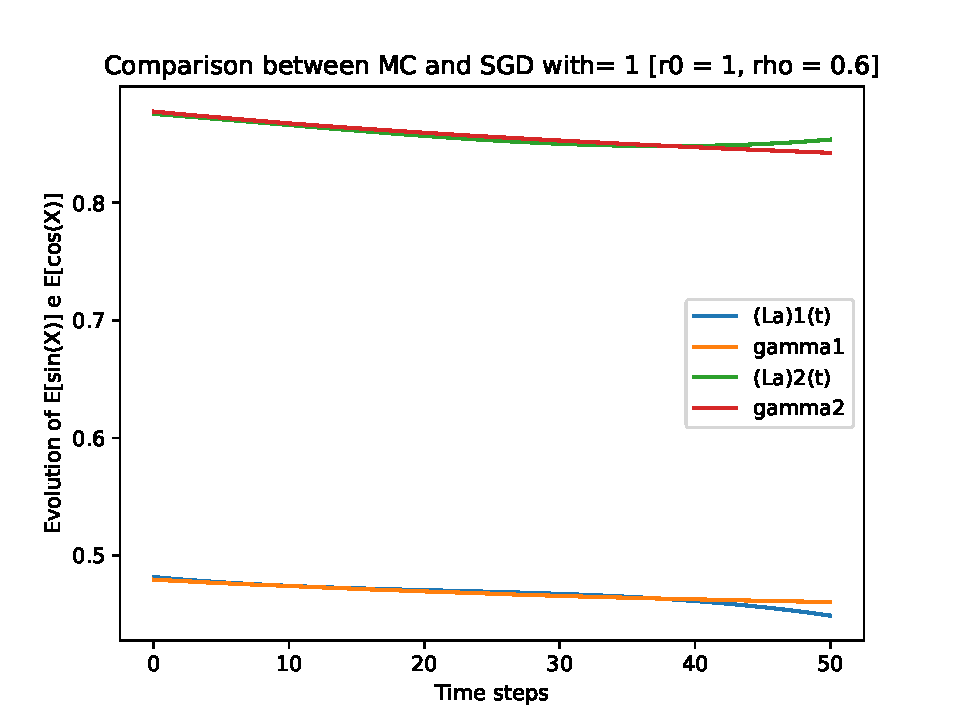
\includegraphics[width=0.9\textwidth]{images/graphs T = 0.5/n = 3, M = 1 sine and cosine.pdf}
\end{figure}
\begin{figure}[H]
\centering
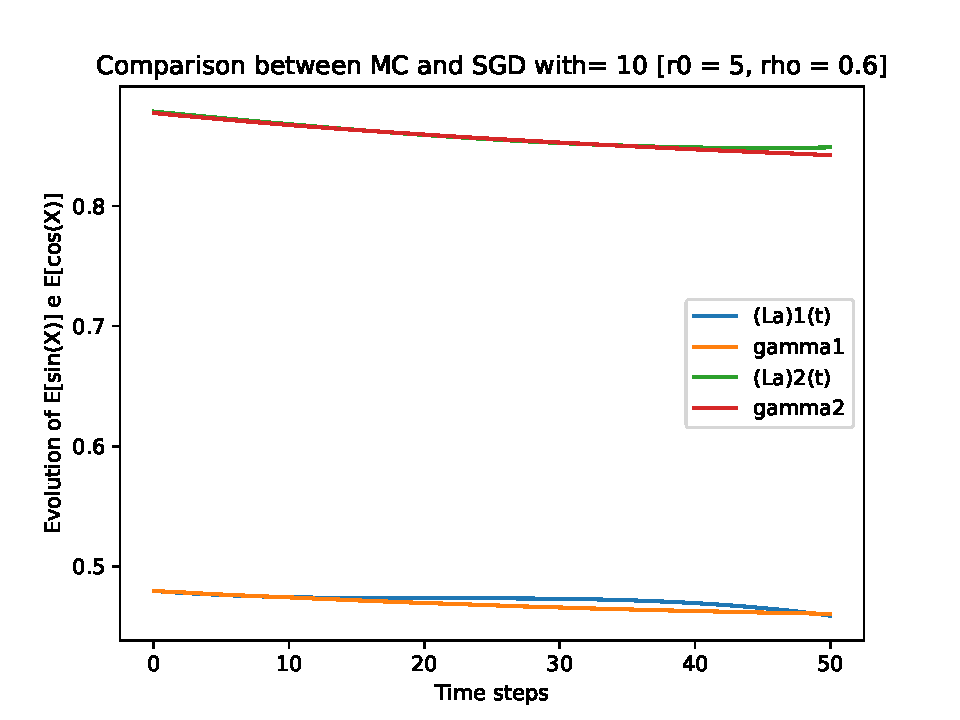
\includegraphics[width=0.9\textwidth]{images/graphs T = 0.5/n = 3, M = 10 sine and cosine.pdf}
\end{figure}
\begin{figure}[H]
\centering
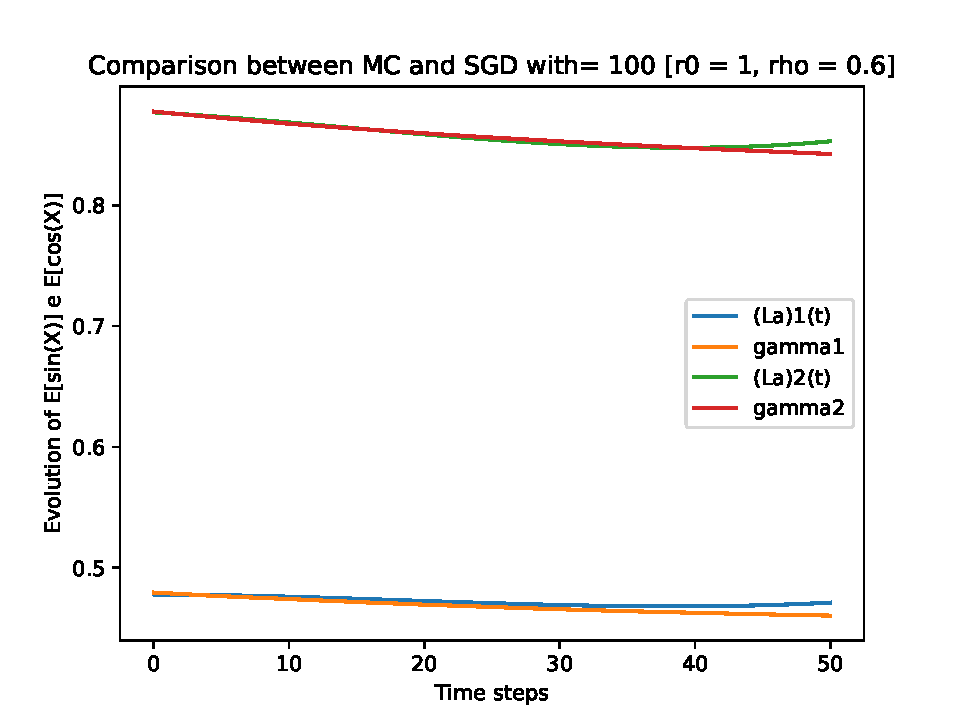
\includegraphics[width=0.9\textwidth]{images/graphs T = 0.5/n = 3, M = 100 sine and cosine.pdf}
\end{figure}
\begin{figure}[H]
\centering
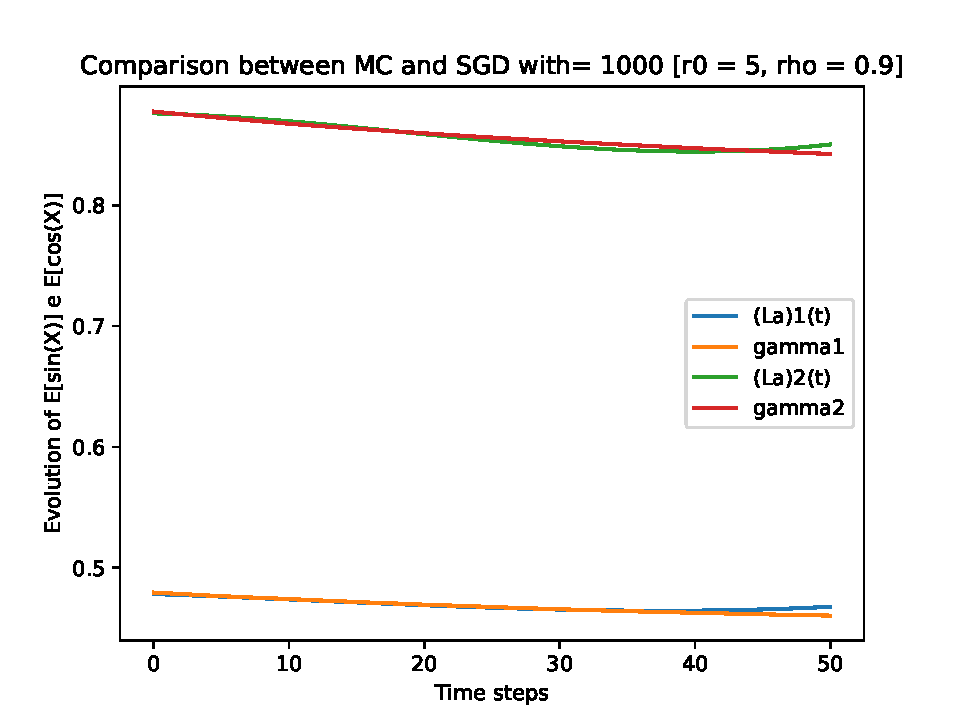
\includegraphics[width=0.9\textwidth]{images/graphs T = 0.5/n = 3, M = 1000 sine and cosine.pdf}
\end{figure}
\begin{figure}[H]
\centering
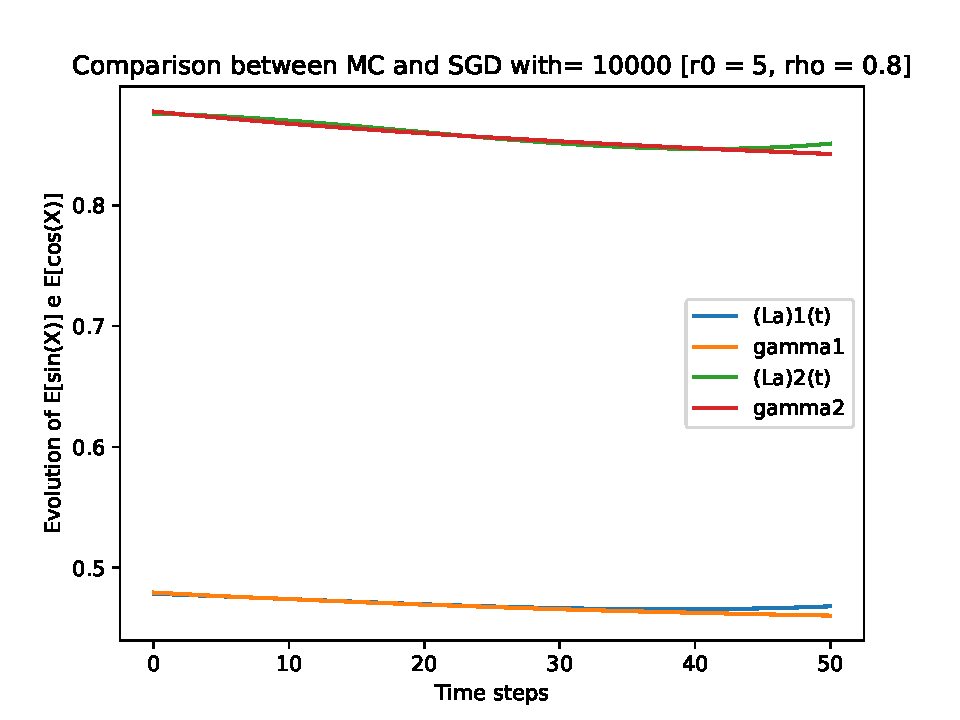
\includegraphics[width=0.9\textwidth]{images/graphs T = 0.5/n = 3, M = 10000 sine and cosine.pdf}
\end{figure}
\newpage
\section*{Case n = 4}  
\begin{table}[H]
\centering
\addtolength{\leftskip}{-1.5cm}
\addtolength{\rightskip}{-1.5cm}
\begin{tabular}{|c|lll|}
\hline
$ $ & $r_0 = 1$ & $r_0 = 5$ & $r_0 = 10$ \\
\hline
$\rho = 0.6$ & 1.72 & 2.90 & 4.55 \\

$\rho = 0.7$ & 1.45 & 1.78 & 2.92 \\

$\rho = 0.8$ & 15.90 & 2.54 & 2.16 \\

$\rho = 0.9$ & 56.10 & 1.97 & 1.70 \\
\hline
\end{tabular}
\caption{Average execution
 times (in seconds $s$) with $M = 1$}
\end{table}
\begin{table}[H]
\centering
\addtolength{\leftskip}{-1.5cm}
\addtolength{\rightskip}{-1.5cm}
\begin{tabular}{|c|lllllllll|}
\hline
$ $ & $r_0 = 1$ & $r_0 = 1$ & $r_0 = 1$ & $r_0 = 5$ & $r_0 = 5$ & $r_0 = 5$ & $r_0 = 10$ & $r_0 = 10$ & $r_0 = 10$  \\
$ $ & min & max & average & min & max & average & min & max & average \\ 
\hline
$\rho = 0.6$ & 60 & 2080 & 484 & 270 & 1460 & 819 & 950 & 1680 & 1288 \\

$\rho = 0.7$ & 120 & 1350 & 412 & 150 & 850 & 505 & 350 & 1620 & 828\\

$\rho = 0.8$ & 120 & 22300 & 4501 & 250 & 1480 & 720 & 230 & 1510 & 609\\

$\rho = 0.9$ & 190 & 49999 & 15893.9 & 60 & 1520 & 560 & 210 & 1180 & 481\\
\hline
\end{tabular}
\caption{Number of iterations $m$ to achieve convergence with $M = 1$}
\end{table}
\begin{table}[H]
\centering
\addtolength{\leftskip}{-1.5cm}
\addtolength{\rightskip}{-1.5cm}
\begin{tabular}{|c|lll|}
\hline
$ $ & $r_0 = 1$ & $r_0 = 5$ & $r_0 = 10$ \\
\hline
$\rho = 0.6$ & 0.26 & 0.39 & 0.77 \\

$\rho = 0.7$ & 0.57 & 0.33 & 0.57 \\

$\rho = 0.8$ & 0.42 & 0.43 & 0.34 \\

$\rho = 0.9$ & 6.07 & 0.22 & 0.31 \\
\hline
\end{tabular}
\caption{Average execution
 times (in seconds $s$) with $M = 10$}
\end{table}
\begin{table}[H]
\centering
\addtolength{\leftskip}{-1.5cm}
\addtolength{\rightskip}{-1.5cm}
\begin{tabular}{|c|lllllllll|}
\hline
$ $ & $r_0 = 1$ & $r_0 = 1$ & $r_0 = 1$ & $r_0 = 5$ & $r_0 = 5$ & $r_0 = 5$ & $r_0 = 10$ & $r_0 = 10$ & $r_0 = 10$  \\
$ $ & min & max & average & min & max & average & min & max & average \\ 
\hline
$\rho = 0.6$ & 30 & 150 & 64 & 40 & 160 & 95 & 70 & 310 & 188\\

$\rho = 0.7$ & 30 & 450 & 139 & 20 & 150 & 80 & 40 & 220 & 140\\

$\rho = 0.8$ & 30 & 210 & 104 & 30 & 230 & 104 & 20 & 200 & 84\\

$\rho = 0.9$ & 20 & 6840 & 1486 & 10 & 120 & 54 & 30 & 180 & 76\\
\hline
\end{tabular}
\caption{Number of iterations $m$ to achieve convergence with $M = 10$}
\end{table}
\begin{table}[H]
\centering
\addtolength{\leftskip}{-1.5cm}
\addtolength{\rightskip}{-1.5cm}
\begin{tabular}{|c|lll|}
\hline
$ $ & $r_0 = 1$ & $r_0 = 5$ & $r_0 = 10$ \\
\hline
$\rho = 0.6$ & 0.16 & 0.12 & 0.23\\

$\rho = 0.7$ & 0.21 & 0.13 & 0.26 \\

$\rho = 0.8$ & 0.32 & 0.12 & 0.15 \\

$\rho = 0.9$ & 0.55 & 0.13 & 0.17 \\
\hline
\end{tabular}
\caption{Average execution
 times (in seconds $s$) with $M = 100$}
\end{table}
\begin{table}[H]
\centering
\addtolength{\leftskip}{-1.5cm}
\addtolength{\rightskip}{-1.5cm}
\begin{tabular}{|c|lllllllll|}
\hline
$ $ & $r_0 = 1$ & $r_0 = 1$ & $r_0 = 1$ & $r_0 = 5$ & $r_0 = 5$ & $r_0 = 5$ & $r_0 = 10$ & $r_0 = 10$ & $r_0 = 10$  \\
$ $ & min & max & average & min & max & average & min & max & average \\ 
\hline
$\rho = 0.6$ & 20 & 40 & 24 & 10 & 30 & 18 & 10 & 80 & 34\\

$\rho = 0.7$ & 20 & 90 & 31 & 10 & 50 & 19 & 20 & 100 & 38\\

$\rho = 0.8$ & 20 & 100 & 48 & 10 & 30 & 17 & 10 & 30 & 21\\

$\rho = 0.9$ & 40 & 180 & 82 & 10 & 30 & 20 & 10 & 40 & 25\\
\hline
\end{tabular}
\caption{Number of iterations $m$ to achieve convergence with $M = 100$}
\end{table}
\begin{table}[H]
\centering
\addtolength{\leftskip}{-1.5cm}
\addtolength{\rightskip}{-1.5cm}
\begin{tabular}{|c|lll|}
\hline
$ $ & $r_0 = 1$ & $r_0 = 5$ & $r_0 = 10$ \\
\hline
$\rho = 0.6$ & 0.56 & 0.13 & 0.2 \\

$\rho = 0.7$ & 0.66 & 0.13 & 0.20 \\

$\rho = 0.8$ & 0.99 & 0.14 & 0.16 \\

$\rho = 0.9$ & 1.53 & 0.15 & 0.14 \\
\hline
\end{tabular}
\caption{Average execution
 times (in seconds $s$) with $M = 1000$}
\end{table}
\begin{table}[H]
\centering
\addtolength{\leftskip}{-1.5cm}
\addtolength{\rightskip}{-1.5cm}
\begin{tabular}{|c|lllllllll|}
\hline
$ $ & $r_0 = 1$ & $r_0 = 1$ & $r_0 = 1$ & $r_0 = 5$ & $r_0 = 5$ & $r_0 = 5$ & $r_0 = 10$ & $r_0 = 10$ & $r_0 = 10$  \\
$ $ & min & max & average & min & max & average & min & max & average \\ 
\hline
$\rho = 0.6$ & 10 & 19 & 13.1 & 2 & 7 & 2.9 & 4 & 6 & 4.6\\

$\rho = 0.7$ & 13 & 20 & 15.4 & 2 & 5 & 2.9 & 4 & 6 & 4.6\\

$\rho = 0.8$ & 19 & 37 & 23.3 & 2 & 11 & 3.2 & 3 & 4 & 3.8\\

$\rho = 0.9$ & 30 & 44 & 35.9 & 2 & 16 & 3.6 & 3 & 4 & 3.3\\
\hline
\end{tabular}
\caption{Number of iterations $m$ to achieve convergence with $M = 1000$}
\end{table}
\begin{table}[H]
\centering
\addtolength{\leftskip}{-1.5cm}
\addtolength{\rightskip}{-1.5cm}
\begin{tabular}{|c|lll|}
\hline
$ $ & $r_0 = 1$ & $r_0 = 5$ & $r_0 = 10$ \\
\hline
$\rho = 0.6$ & 6.26 & 1.07 & 2.12 \\

$\rho = 0.7$ & 7.68 & 1.07 & 2.14 \\

$\rho = 0.8$ & 10.63 & 1.06 & 1.71 \\

$\rho = 0.9$ & 17.56 & 1.06 & 1.66 \\
\hline
\end{tabular}
\caption{Average execution
 times (in seconds $s$) with $M = 10000$}
\end{table}
\begin{table}[H]
\centering
\addtolength{\leftskip}{-1.5cm}
\addtolength{\rightskip}{-1.5cm}
\begin{tabular}{|c|lllllllll|}
\hline
$ $ & $r_0 = 1$ & $r_0 = 1$ & $r_0 = 1$ & $r_0 = 5$ & $r_0 = 5$ & $r_0 = 5$ & $r_0 = 10$ & $r_0 = 10$ & $r_0 = 10$  \\
$ $ & min & max & average & min & max & average & min & max & average \\ 
\hline
$\rho = 0.6$ & 11 & 12 & 11.6 & 2 & 2 & 2 & 4 & 4 & 4\\

$\rho = 0.7$ & 14 & 15 & 14.3 & 2 & 2 & 2 & 4 & 4 & 4\\

$\rho = 0.8$ & 18 & 21 & 19.7 & 2 & 2 & 2 & 3 & 4 & 3.2\\

$\rho = 0.9$ & 29 & 35 & 32.7 & 2 & 2 & 2 & 3 & 4 & 3.1\\
\hline
\end{tabular}
\caption{Number of iterations $m$ to achieve convergence with $M = 10000$}
\end{table}
\begin{figure}[H]
\centering
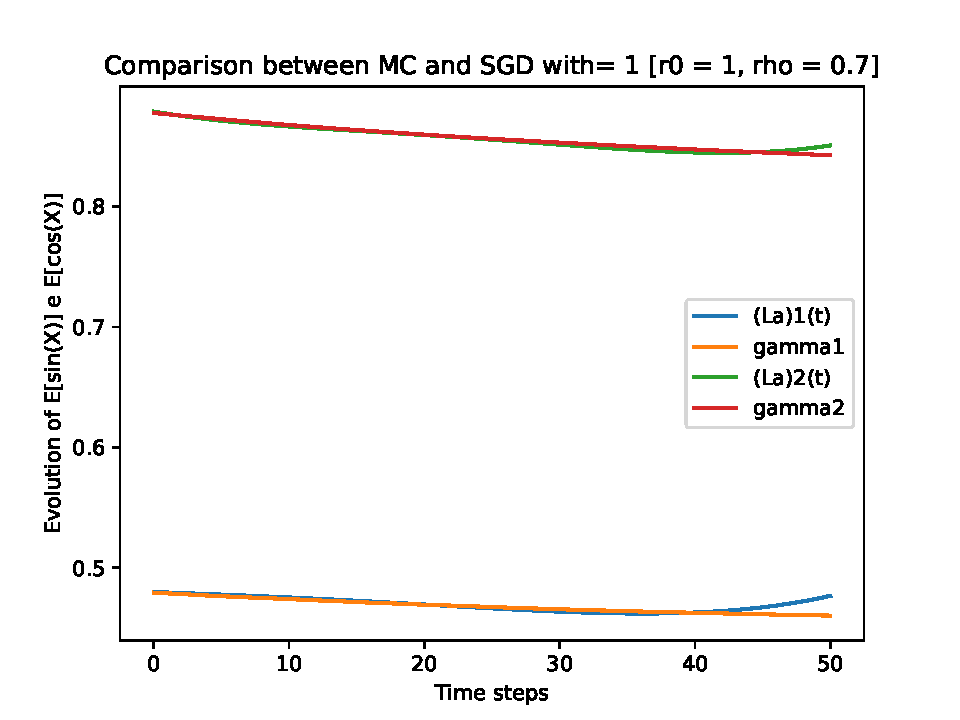
\includegraphics[width=0.9\textwidth]{images/graphs T = 0.5/n = 4, M = 1 sine and cosine.pdf}
\end{figure}
\begin{figure}[H]
\centering
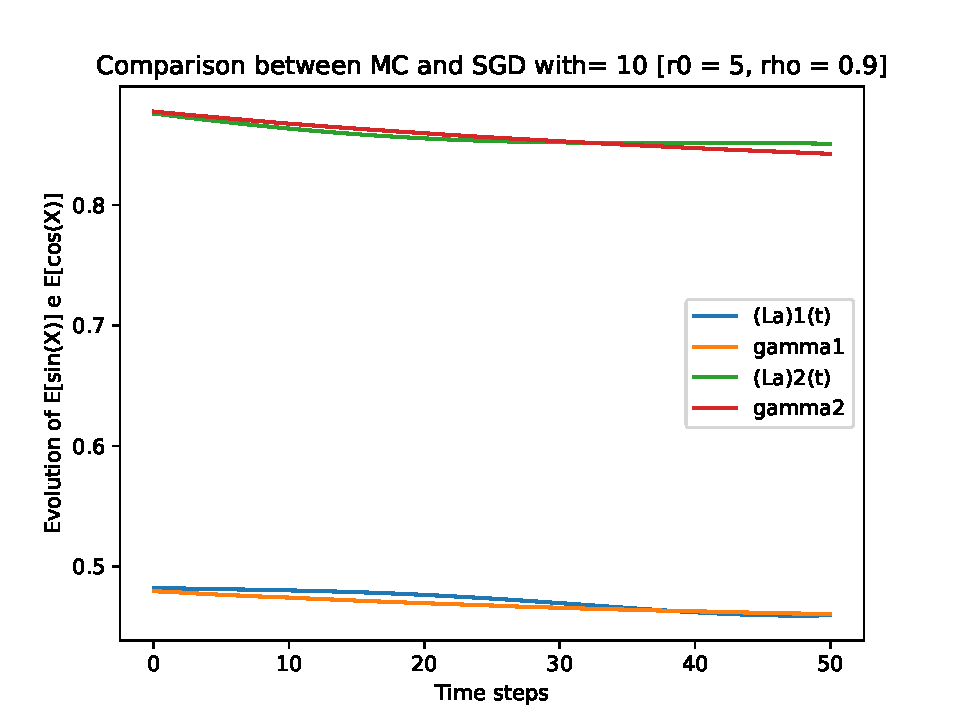
\includegraphics[width=0.9\textwidth]{images/graphs T = 0.5/n = 4, M = 10 sine and cosine.pdf}
\end{figure}
\begin{figure}[H]
\centering
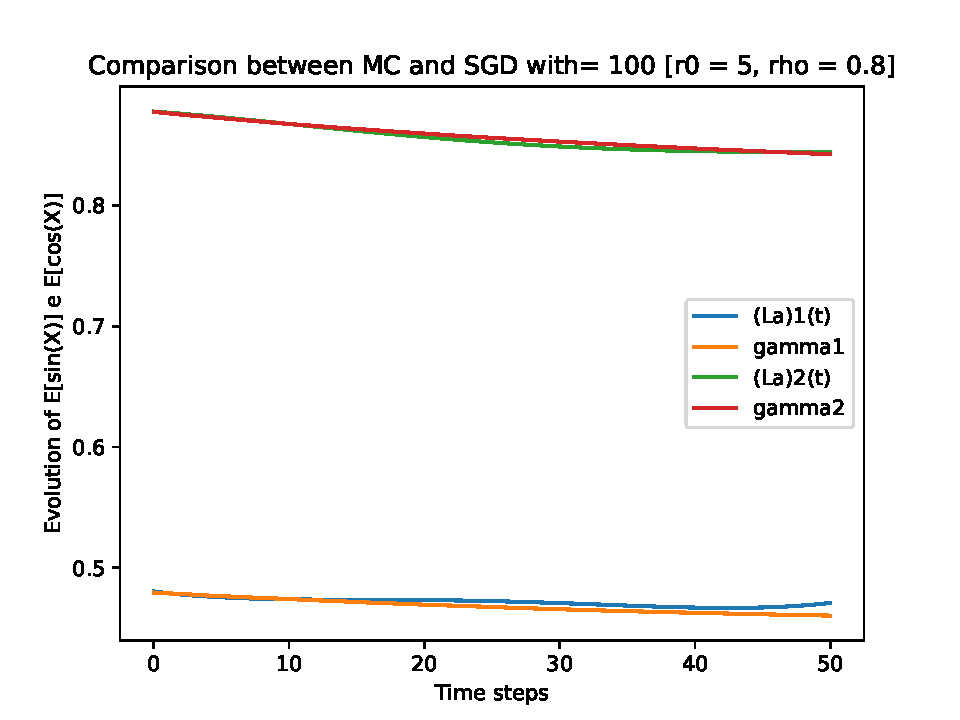
\includegraphics[width=0.9\textwidth]{images/graphs T = 0.5/n = 4, M = 100 sine and cosine.pdf}
\end{figure}
\begin{figure}[H]
\centering
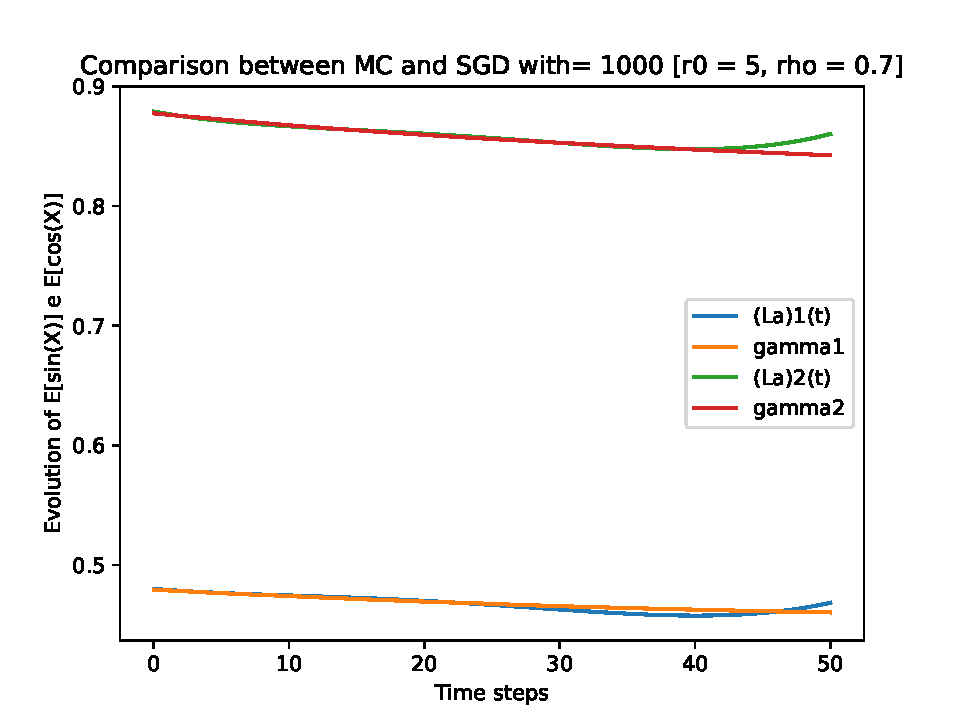
\includegraphics[width=0.9\textwidth]{images/graphs T = 0.5/n = 4, M = 1000 sine and cosine.pdf}
\end{figure}
\begin{figure}[H]
\centering
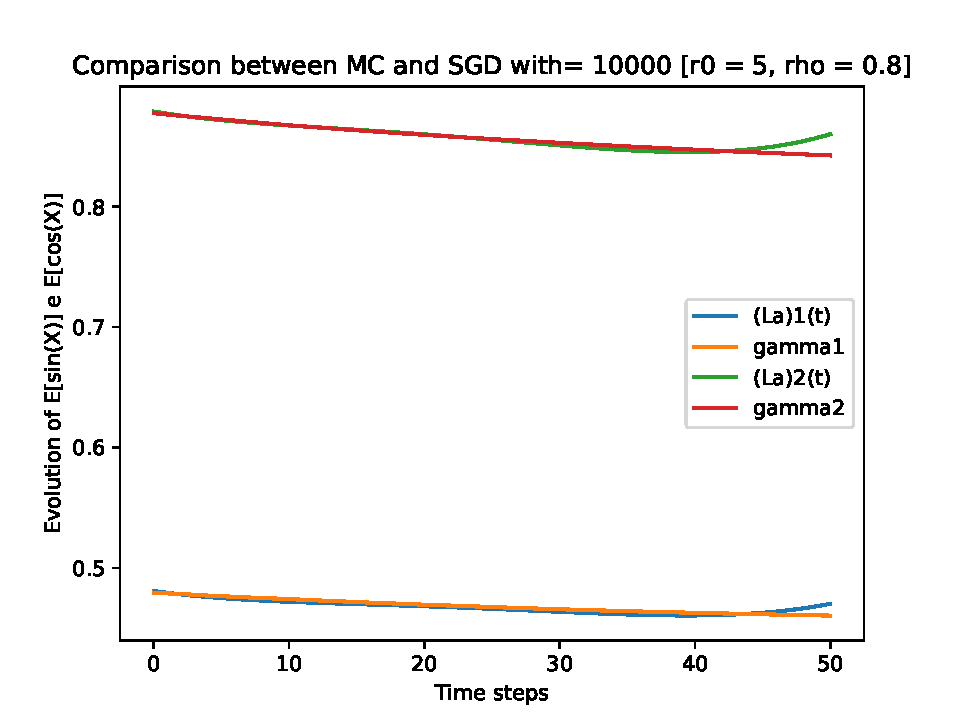
\includegraphics[width=0.9\textwidth]{images/graphs T = 0.5/n = 4, M = 10000 sine and cosine.pdf}
\end{figure}
\newpage
\section*{Case n = 5} 
\begin{table}[H]
\centering
\addtolength{\leftskip}{-1.5cm}
\addtolength{\rightskip}{-1.5cm}
\begin{tabular}{|c|lll|}
\hline
$ $ & $r_0 = 1$ & $r_0 = 5$ & $r_0 = 10$ \\
\hline
$\rho = 0.6$ & 1.36 & 4.12 & 8.9 \\

$\rho = 0.7$ & 2.67 & 2.78 & 3.51 \\

$\rho = 0.8$ & 4.66 & 2.35 & 2.92 \\

$\rho = 0.9$ & 90.29 & 3.76 & 2.65 \\
\hline
\end{tabular}
\caption{Average execution
 times (in seconds $s$) with $M = 1$}
\end{table}
\begin{table}[H]
\centering
\addtolength{\leftskip}{-1.5cm}
\addtolength{\rightskip}{-1.5cm}
\begin{tabular}{|c|lllllllll|}
\hline
$ $ & $r_0 = 1$ & $r_0 = 1$ & $r_0 = 1$ & $r_0 = 5$ & $r_0 = 5$ & $r_0 = 5$ & $r_0 = 10$ & $r_0 = 10$ & $r_0 = 10$  \\
$ $ & min & max & average & min & max & average & min & max & average \\ 
\hline
$\rho = 0.6$ & 130 & 890 & 371 & 370 & 1760 & 866 & 610 & 2870 & 1714 \\

$\rho = 0.7$ & 110 & 2470 & 729 & 240 & 1070 & 589 & 420 & 1050 & 753\\

$\rho = 0.8$ & 90 & 4260 & 1271 & 130 & 1190 & 496 & 240 & 1100 & 613\\

$\rho = 0.9$ & 440 & 49999 & 22338.7 & 200 & 1330 & 661 & 160 & 1380 & 565\\
\hline
\end{tabular}
\caption{Number of iterations $m$ to achieve convergence with $M = 1$}
\end{table}
\begin{table}[H]
\centering
\addtolength{\leftskip}{-1.5cm}
\addtolength{\rightskip}{-1.5cm}
\begin{tabular}{|c|lll|}
\hline
$ $ & $r_0 = 1$ & $r_0 = 5$ & $r_0 = 10$ \\
\hline
$\rho = 0.6$ & 0.85 & 0.64 & 1.25 \\

$\rho = 0.7$ & 0.88 & 0.53 & 0.73 \\

$\rho = 0.8$ & 2.96 & 0.61 & 0.37 \\

$\rho = 0.9$ & 2.35 & 0.58 & 0.53 \\
\hline
\end{tabular}
\caption{Average execution
 times (in seconds $s$) with $M = 10$}
\end{table}
\begin{table}[H]
\centering
\addtolength{\leftskip}{-1.5cm}
\addtolength{\rightskip}{-1.5cm}
\begin{tabular}{|c|lllllllll|}
\hline
$ $ & $r_0 = 1$ & $r_0 = 1$ & $r_0 = 1$ & $r_0 = 5$ & $r_0 = 5$ & $r_0 = 5$ & $r_0 = 10$ & $r_0 = 10$ & $r_0 = 10$  \\
$ $ & min & max & average & min & max & average & min & max & average \\ 
\hline
$\rho = 0.6$ & 20 & 400 & 148 & 30 & 290 & 110 & 80 & 340 & 217\\

$\rho = 0.7$ & 20 & 630 & 157 & 20 & 190 & 89 & 40 & 250 & 132\\

$\rho = 0.8$ & 60 & 2110 & 513 & 20 & 280 & 104 & 30 & 100 & 68\\

$\rho = 0.9$ & 110 & 1210 & 411 & 30 & 250 & 103 & 20 & 210 & 93\\
\hline
\end{tabular}
\caption{Number of iterations $m$ to achieve convergence with $M = 10$}
\end{table}
\begin{table}[H]
\centering
\addtolength{\leftskip}{-1.5cm}
\addtolength{\rightskip}{-1.5cm}
\begin{tabular}{|c|lll|}
\hline
$ $ & $r_0 = 1$ & $r_0 = 5$ & $r_0 = 10$ \\
\hline
$\rho = 0.6$ & 0.29 & 0.28 & 0.25 \\

$\rho = 0.7$ & 0.48 & 0.25 & 0.40 \\

$\rho = 0.8$ & 0.98 & 0.18 & 0.38 \\

$\rho = 0.9$ & 1.31 & 0.29 & 0.19 \\
\hline
\end{tabular}
\caption{Average execution
 times (in seconds $s$) with $M = 100$}
\end{table}
\begin{table}[H]
\centering
\addtolength{\leftskip}{-1.5cm}
\addtolength{\rightskip}{-1.5cm}
\begin{tabular}{|c|lllllllll|}
\hline
$ $ & $r_0 = 1$ & $r_0 = 1$ & $r_0 = 1$ & $r_0 = 5$ & $r_0 = 5$ & $r_0 = 5$ & $r_0 = 10$ & $r_0 = 10$ & $r_0 = 10$  \\
$ $ & min & max & average & min & max & average & min & max & average \\ 
\hline
$\rho = 0.6$ & 20 & 40 & 27 & 10 & 60 & 21 & 10 & 40 & 22\\

$\rho = 0.7$ & 30 & 80 & 49 & 10 & 60 & 19 & 10 & 60 & 33\\

$\rho = 0.8$ & 40 & 180 & 85 & 10 & 30 & 16 & 10 & 50 & 30\\

$\rho = 0.9$ & 70 & 180 & 114 & 10 & 60 & 24 & 10 & 40 & 16\\
\hline
\end{tabular}
\caption{Number of iterations $m$ to achieve convergence with $M = 100$}
\end{table}
\begin{table}[H]
\centering
\addtolength{\leftskip}{-1.5cm}
\addtolength{\rightskip}{-1.5cm}
\begin{tabular}{|c|lll|}
\hline
$ $ & $r_0 = 1$ & $r_0 = 5$ & $r_0 = 10$ \\
\hline
$\rho = 0.6$ & 1.41 & 0.22 & 0.30 \\

$\rho = 0.7$ & 1.73 & 0.17 & 0.26 \\

$\rho = 0.8$ & 2.85 & 0.15 & 0.23 \\

$\rho = 0.9$ & 5.33 & 0.19 & 0.28 \\
\hline
\end{tabular}
\caption{Average execution
 times (in seconds $s$) with $M = 1000$}
\end{table}
\begin{table}[H]
\centering
\addtolength{\leftskip}{-1.5cm}
\addtolength{\rightskip}{-1.5cm}
\begin{tabular}{|c|lllllllll|}
\hline
$ $ & $r_0 = 1$ & $r_0 = 1$ & $r_0 = 1$ & $r_0 = 5$ & $r_0 = 5$ & $r_0 = 5$ & $r_0 = 10$ & $r_0 = 10$ & $r_0 = 10$  \\
$ $ & min & max & average & min & max & average & min & max & average \\ 
\hline
$\rho = 0.6$ & 15 & 25 & 18.6 & 1 & 8 & 2.6 & 3 & 6 & 3.8\\

$\rho = 0.7$ & 20 & 24 & 22.5 & 1 & 7 & 2.2 & 3 & 4 & 3.3\\

$\rho = 0.8$ & 32 & 45 & 37.5 & 1 & 4 & 1.9 & 3 & 4 & 3.2\\

$\rho = 0.9$ & 53 & 104 & 70.3 & 1 & 6 & 2.6 & 3 & 6 & 3.5\\
\hline
\end{tabular}
\caption{Number of iterations $m$ to achieve convergence with $M = 1000$}
\end{table}
\begin{table}[H]
\centering
\addtolength{\leftskip}{-1.5cm}
\addtolength{\rightskip}{-1.5cm}
\begin{tabular}{|c|lll|}
\hline
$ $ & $r_0 = 1$ & $r_0 = 5$ & $r_0 = 10$ \\
\hline
$\rho = 0.6$ & 16.95 & 1.42 & 3.38 \\

$\rho = 0.7$ & 23.12 & 1.48 & 3.20 \\

$\rho = 0.8$ & 36.69 & 1.3 & 3.22 \\

$\rho = 0.9$ & 68.4 & 1.13 & 3.13 \\
\hline
\end{tabular}
\caption{Average execution
 times (in seconds $s$) with $M = 10000$}
\end{table}
\begin{table}[H]
\centering
\addtolength{\leftskip}{-1.5cm}
\addtolength{\rightskip}{-1.5cm}
\begin{tabular}{|c|lllllllll|}
\hline
$ $ & $r_0 = 1$ & $r_0 = 1$ & $r_0 = 1$ & $r_0 = 5$ & $r_0 = 5$ & $r_0 = 5$ & $r_0 = 10$ & $r_0 = 10$ & $r_0 = 10$  \\
$ $ & min & max & average & min & max & average & min & max & average \\ 
\hline
$\rho = 0.6$ & 15 & 16 & 15.7 & 1 & 2 & 1.3 & 3 & 4 & 3.1\\

$\rho = 0.7$ & 21 & 23 & 21.5 & 1 & 2 & 1.4 & 3 & 3 & 3\\

$\rho = 0.8$ & 32 & 36 & 34.4 & 1 & 2 & 1.2 & 3 & 3 & 3\\

$\rho = 0.9$ & 59 & 66 & 63.4 & 1 & 1 & 1 & 2 & 3 & 2.9\\
\hline
\end{tabular}
\caption{Number of iterations $m$ to achieve convergence with $M = 10000$}
\end{table}
\begin{figure}[H]
\centering
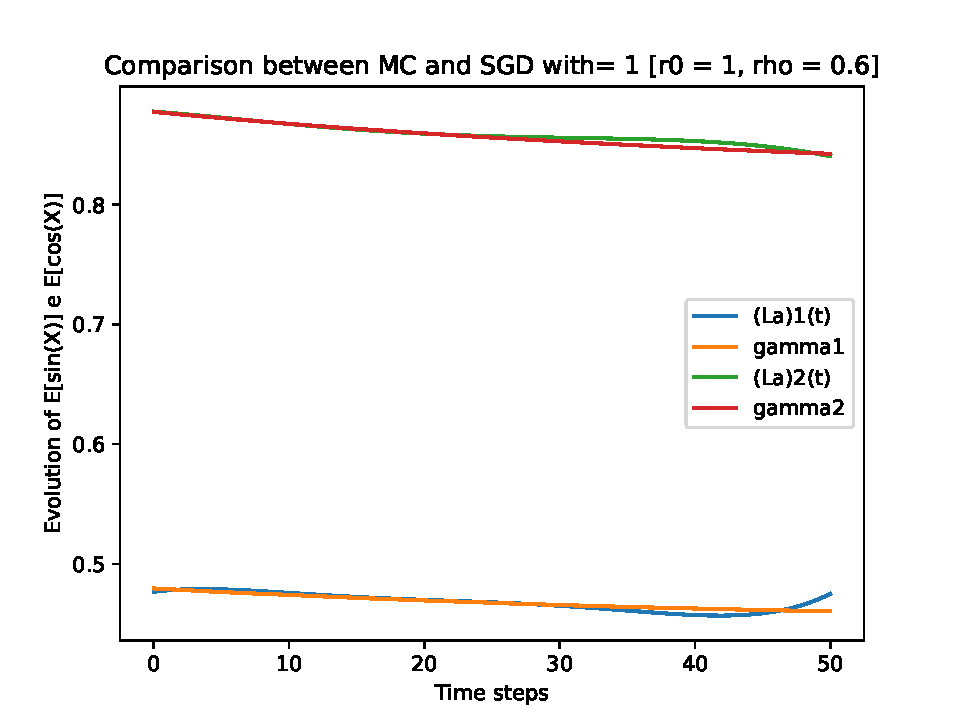
\includegraphics[width=0.9\textwidth]{images/graphs T = 0.5/n = 5, M = 1 sine and cosine.pdf}
\end{figure}
\begin{figure}[H]
\centering
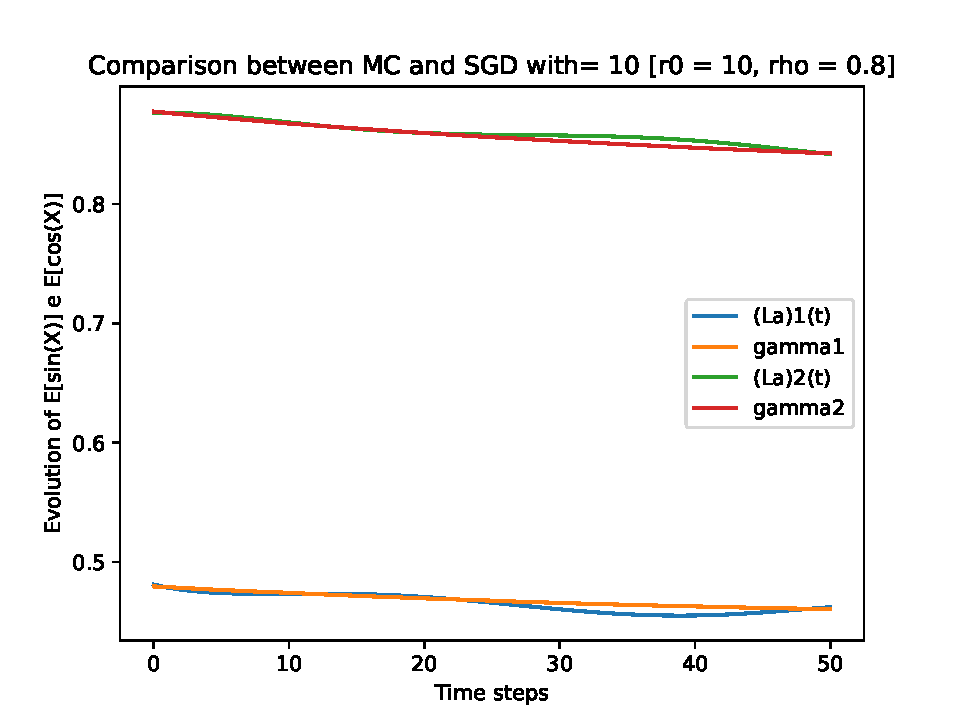
\includegraphics[width=0.9\textwidth]{images/graphs T = 0.5/n = 5, M = 10 sine and cosine.pdf}
\end{figure}
\begin{figure}[H]
\centering
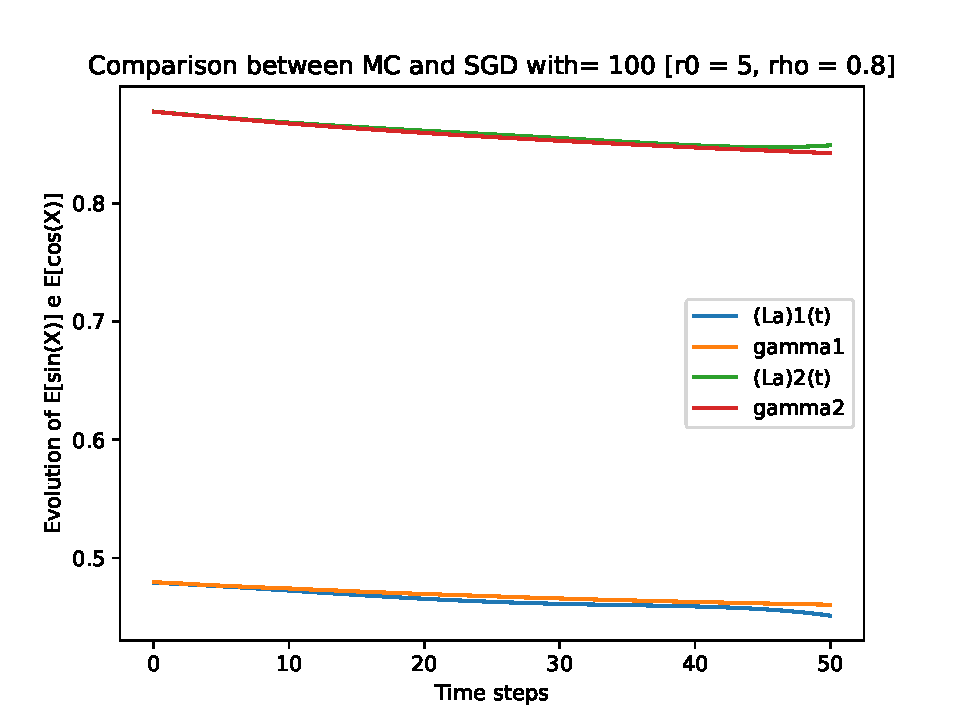
\includegraphics[width=0.9\textwidth]{images/graphs T = 0.5/n = 5, M = 100 sine and cosine.pdf}
\end{figure}
\begin{figure}[H]
\centering
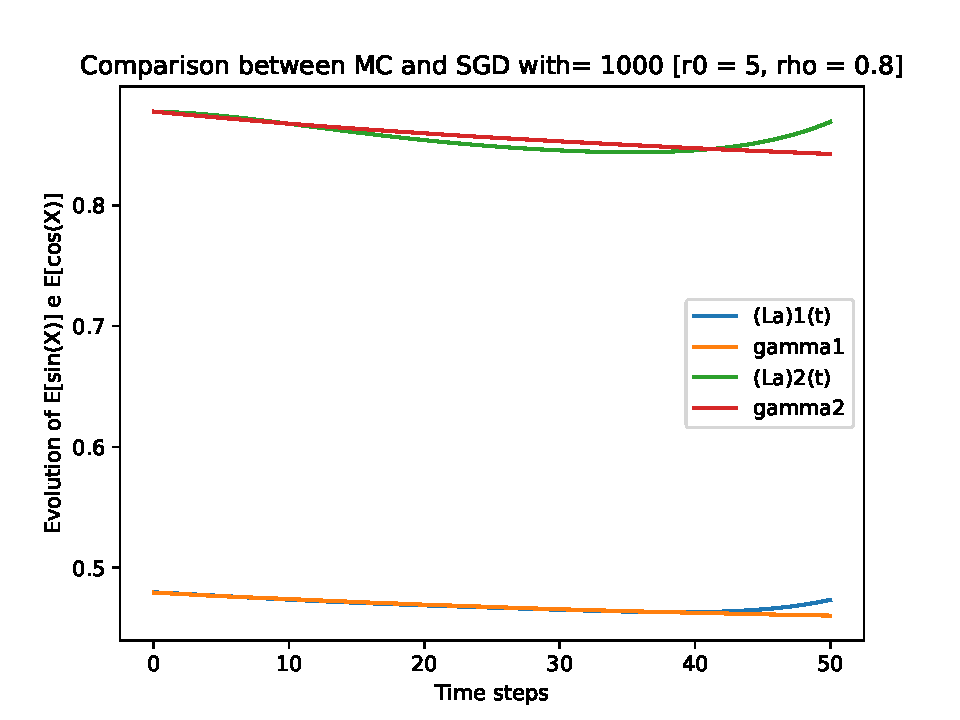
\includegraphics[width=0.9\textwidth]{images/graphs T = 0.5/n = 5, M = 1000 sine and cosine.pdf}
\end{figure}
\begin{figure}[H]
\centering
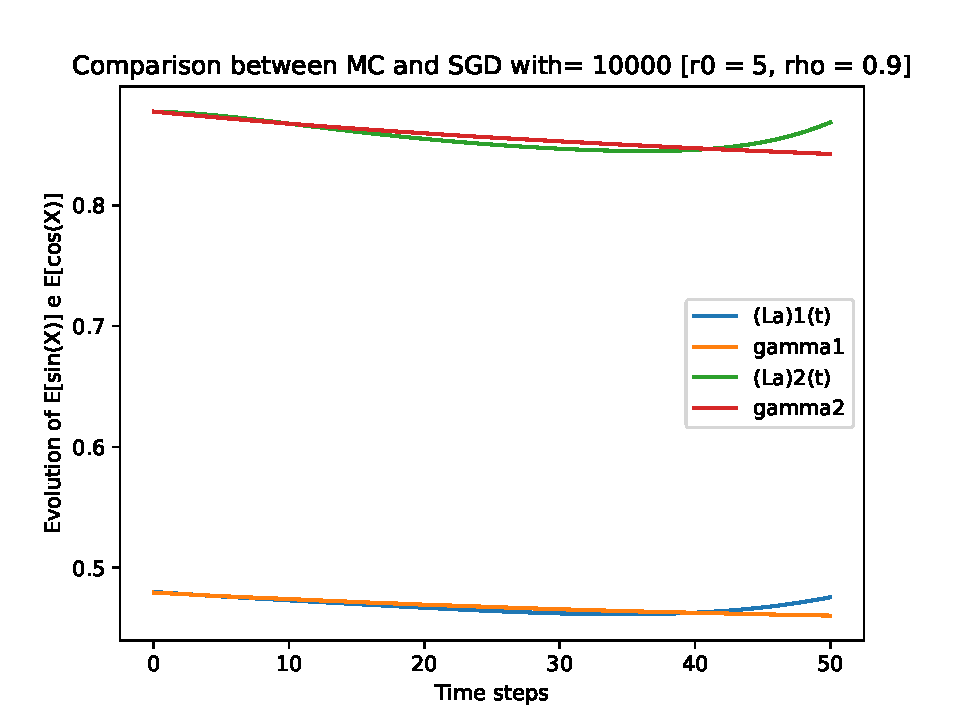
\includegraphics[width=0.9\textwidth]{images/graphs T = 0.5/n = 5, M = 10000 sine and cosine.pdf}
\end{figure}
\newpage
\section*{Case n = 6}  
\begin{table}[H]
\centering
\addtolength{\leftskip}{-1.5cm}
\addtolength{\rightskip}{-1.5cm}
\begin{tabular}{|c|lll|}
\hline
$ $ & $r_0 = 1$ & $r_0 = 5$ & $r_0 = 10$ \\
\hline
$\rho = 0.6$ & 5.18 & 4.60 & 8.74 \\

$\rho = 0.7$ & 4.49 & 4.45 & 5.47 \\

$\rho = 0.8$ & 19.83 & 5.0 & 4.59 \\

$\rho = 0.9$ & 147.74 & 9.4 & 4.57 \\
\hline
\end{tabular}
\caption{Average execution
 times (in seconds $s$) with $M = 1$}
\end{table}
\begin{table}[H]
\centering
\addtolength{\leftskip}{-1.5cm}
\addtolength{\rightskip}{-1.5cm}
\begin{tabular}{|c|lllllllll|}
\hline
$ $ & $r_0 = 1$ & $r_0 = 1$ & $r_0 = 1$ & $r_0 = 5$ & $r_0 = 5$ & $r_0 = 5$ & $r_0 = 10$ & $r_0 = 10$ & $r_0 = 10$  \\
$ $ & min & max & average & min & max & average & min & max & average \\ 
\hline
$\rho = 0.6$ & 130 & 2650 & 864 & 260 & 1430 & 791 & 410 &  2140 & 1250 \\

$\rho = 0.7$ & 80 & 2080 & 731 & 210 & 1060 & 782 & 260 & 1370 & 766\\

$\rho = 0.8$ & 100 & 8230 & 3184 & 200 & 1550 & 809 & 260 & 1720 & 663\\

$\rho = 0.9$ & 180 & 49999 & 25371.6 & 220 & 6350 & 1360 & 190 & 2440 & 765\\
\hline
\end{tabular}
\caption{Number of iterations $m$ to achieve convergence with $M = 1$}
\end{table}
\begin{table}[H]
\centering
\addtolength{\leftskip}{-1.5cm}
\addtolength{\rightskip}{-1.5cm}
\begin{tabular}{|c|lll|}
\hline
$ $ & $r_0 = 1$ & $r_0 = 5$ & $r_0 = 10$ \\
\hline
$\rho = 0.6$ & 0.68 & 0.33 & 0.74 \\

$\rho = 0.7$ & 0.56 & 0.44 & 0.49 \\

$\rho = 0.8$ & 2.31 & 0.53 & 0.51 \\

$\rho = 0.9$ & 24.46 & 0.48 & 0.39 \\
\hline
\end{tabular}
\caption{Average execution
 times (in seconds $s$) with $M = 10$}
\end{table}
\begin{table}[H]
\centering
\addtolength{\leftskip}{-1.5cm}
\addtolength{\rightskip}{-1.5cm}
\begin{tabular}{|c|lllllllll|}
\hline
$ $ & $r_0 = 1$ & $r_0 = 1$ & $r_0 = 1$ & $r_0 = 5$ & $r_0 = 5$ & $r_0 = 5$ & $r_0 = 10$ & $r_0 = 10$ & $r_0 = 10$  \\
$ $ & min & max & average & min & max & average & min & max & average \\ 
\hline
$\rho = 0.6$ & 30 & 240 & 89 & 20 & 180 & 75 & 30 & 380 & 167\\

$\rho = 0.7$ & 40 & 160 & 77 & 40 & 210 & 99 & 40 & 160 & 110\\

$\rho = 0.8$ & 50 & 1080 & 329 & 40 & 300 & 119 & 40 & 290 & 116\\

$\rho = 0.9$ & 120 & 21270 & 4210 & 10 & 240 & 108 & 30 & 220 & 89\\
\hline
\end{tabular}
\caption{Number of iterations $m$ to achieve convergence with $M = 10$}
\end{table}
\begin{table}[H]
\centering
\addtolength{\leftskip}{-1.5cm}
\addtolength{\rightskip}{-1.5cm}
\begin{tabular}{|c|lll|}
\hline
$ $ & $r_0 = 1$ & $r_0 = 5$ & $r_0 = 10$ \\
\hline
$\rho = 0.6$ & 0.32 & 0.19 & 0.19 \\

$\rho = 0.7$ & 0.64 & 0.13 & 0.25 \\

$\rho = 0.8$ & 0.64 & 0.14 & 0.18 \\

$\rho = 0.9$ & 1.54 & 0.16 & 0.17 \\
\hline
\end{tabular}
\caption{Average execution
 times (in seconds $s$) with $M = 100$}
\end{table}
\begin{table}[H]
\centering
\addtolength{\leftskip}{-1.5cm}
\addtolength{\rightskip}{-1.5cm}
\begin{tabular}{|c|lllllllll|}
\hline
$ $ & $r_0 = 1$ & $r_0 = 1$ & $r_0 = 1$ & $r_0 = 5$ & $r_0 = 5$ & $r_0 = 5$ & $r_0 = 10$ & $r_0 = 10$ & $r_0 = 10$  \\
$ $ & min & max & average & min & max & average & min & max & average \\ 
\hline
$\rho = 0.6$ & 30 & 130 & 41 & 10 & 40 & 24 & 10 & 50 & 24\\

$\rho = 0.7$ & 40 & 290 & 81 & 10 & 30 & 16 & 10 & 60 & 31\\

$\rho = 0.8$ & 40 & 120 & 81 & 10 & 60 & 18 & 10 & 40 & 23\\

$\rho = 0.9$ & 110 & 300 & 196 & 10 & 60 & 20 & 10 & 40 & 22\\
\hline
\end{tabular}
\caption{Number of iterations $m$ to achieve convergence with $M = 100$}
\end{table}
\begin{table}[H]
\centering
\addtolength{\leftskip}{-1.5cm}
\addtolength{\rightskip}{-1.5cm}
\begin{tabular}{|c|lll|}
\hline
$ $ & $r_0 = 1$ & $r_0 = 5$ & $r_0 = 10$ \\
\hline
$\rho = 0.6$ & 1.28 & 0.13 & 0.20 \\

$\rho = 0.7$ & 1.87 & 0.12 & 0.19 \\

$\rho = 0.8$ & 2.90 & 0.16 & 0.13 \\

$\rho = 0.9$ & 6.89 & 0.11 & 0.16 \\
\hline
\end{tabular}
\caption{Average execution
 times (in seconds $s$) with $M = 1000$}
\end{table}
\begin{table}[H]
\centering
\addtolength{\leftskip}{-1.5cm}
\addtolength{\rightskip}{-1.5cm}
\begin{tabular}{|c|lllllllll|}
\hline
$ $ & $r_0 = 1$ & $r_0 = 1$ & $r_0 = 1$ & $r_0 = 5$ & $r_0 = 5$ & $r_0 = 5$ & $r_0 = 10$ & $r_0 = 10$ & $r_0 = 10$  \\
$ $ & min & max & average & min & max & average & min & max & average \\ 
\hline
$\rho = 0.6$ & 22 & 29 & 23.7 & 1 & 4 & 2.5 & 3 & 8 & 3.8\\

$\rho = 0.7$ & 31 & 43 & 34.6 & 1 & 4 & 2.1 & 2 & 7 & 3.5\\

$\rho = 0.8$ & 50 & 56 & 53.4 & 1 & 7 & 2.9 & 2 & 4 & 2.5\\

$\rho = 0.9$ & 105 & 174 & 127.3 & 1 & 6 & 2 & 2 & 4 & 2.9\\
\hline
\end{tabular}
\caption{Number of iterations $m$ to achieve convergence with $M = 1000$}
\end{table}
\begin{table}[H]
\centering
\addtolength{\leftskip}{-1.5cm}
\addtolength{\rightskip}{-1.5cm}
\begin{tabular}{|c|lll|}
\hline
$ $ & $r_0 = 1$ & $r_0 = 5$ & $r_0 = 10$ \\
\hline
$\rho = 0.6$ & 16.77 & 0.77 & 1.92 \\

$\rho = 0.7$ & 24.63 & 1.00 & 1.61 \\

$\rho = 0.8$ & 41.76 & 0.77 & 1.61 \\

$\rho = 0.9$ & 93.11 & 0.85 & 1.54 \\
\hline
\end{tabular}
\caption{Average execution
 times (in seconds $s$) with $M = 10000$}
\end{table}
\begin{table}[H]
\centering
\addtolength{\leftskip}{-1.5cm}
\addtolength{\rightskip}{-1.5cm}
\begin{tabular}{|c|lllllllll|}
\hline
$ $ & $r_0 = 1$ & $r_0 = 1$ & $r_0 = 1$ & $r_0 = 5$ & $r_0 = 5$ & $r_0 = 5$ & $r_0 = 10$ & $r_0 = 10$ & $r_0 = 10$  \\
$ $ & min & max & average & min & max & average & min & max & average \\ 
\hline
$\rho = 0.6$ & 21 & 23 & 21.8 & 1 & 1 & 1 & 2 & 3 & 2.5\\

$\rho = 0.7$ & 31 & 34 & 31.9 & 1 & 2 & 1.3 & 2 & 3 & 2.1\\

$\rho = 0.8$ & 52 & 59 & 54.4 & 1 & 1 & 1 & 2 & 3 & 2.1\\

$\rho = 0.9$ & 114 & 128 & 121.3 & 1 & 2 & 1.1 & 2 & 2 & 2\\
\hline
\end{tabular}
\caption{Number of iterations $m$ to achieve convergence with $M = 10000$}
\end{table}
\begin{figure}[H]
\centering
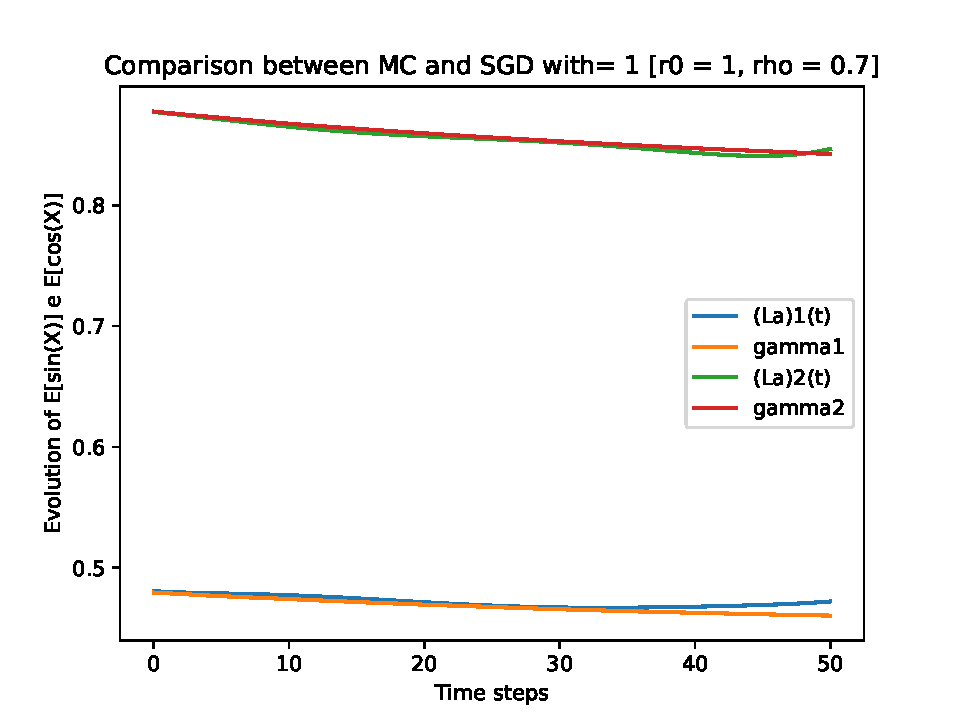
\includegraphics[width=0.9\textwidth]{images/graphs T = 0.5/n = 6, M = 1 sine and cosine.pdf}
\end{figure}
\begin{figure}[H]
\centering
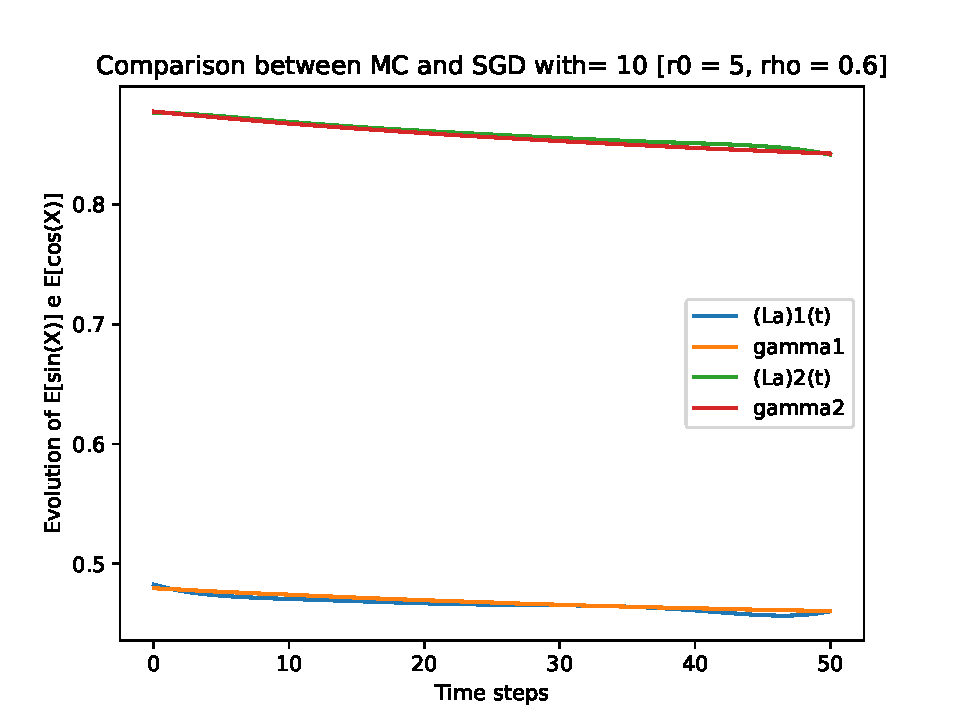
\includegraphics[width=0.9\textwidth]{images/graphs T = 0.5/n = 6, M = 10 sine and cosine.pdf}
\end{figure}
\begin{figure}[H]
\centering
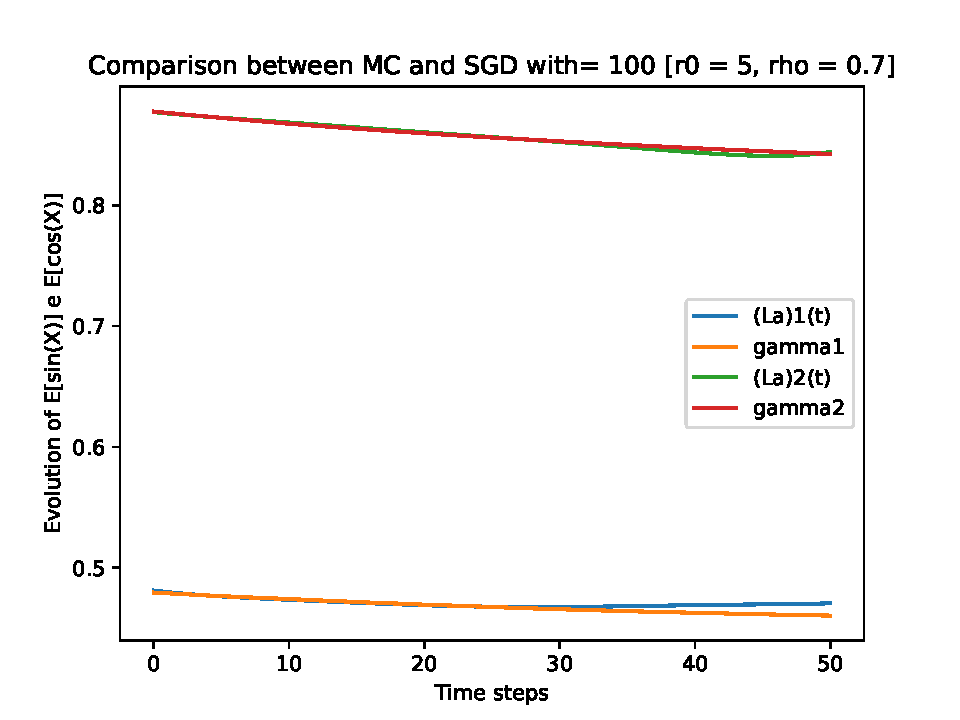
\includegraphics[width=0.9\textwidth]{images/graphs T = 0.5/n = 6, M = 100 sine and cosine.pdf}
\end{figure}
\begin{figure}[H]
\centering
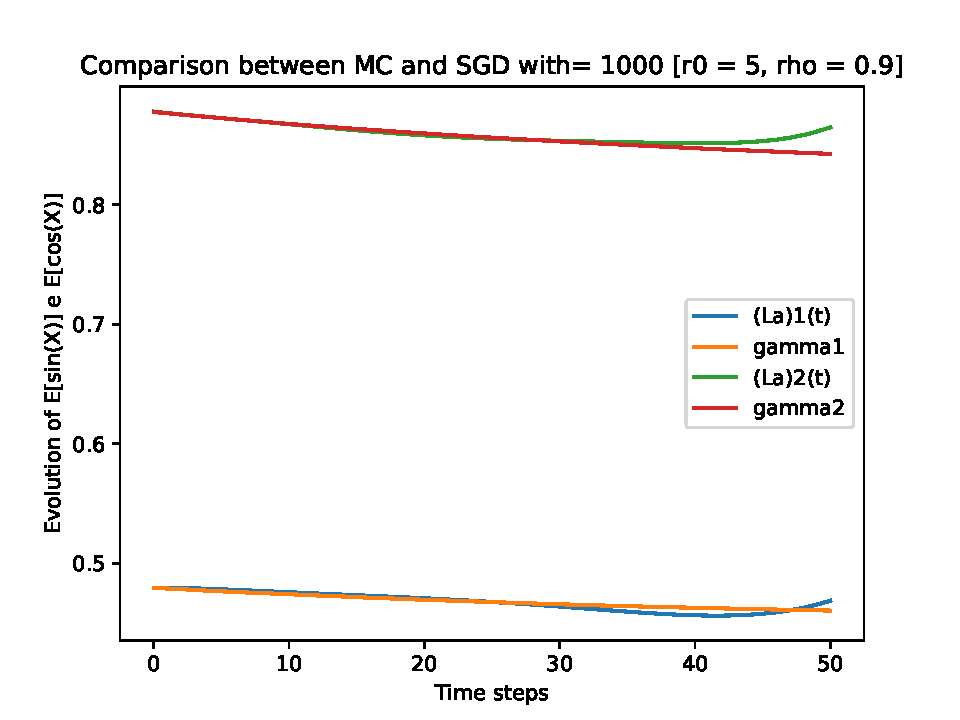
\includegraphics[width=0.9\textwidth]{images/graphs T = 0.5/n = 6, M = 1000 sine and cosine.pdf}
\end{figure}
\begin{figure}[H]
\centering
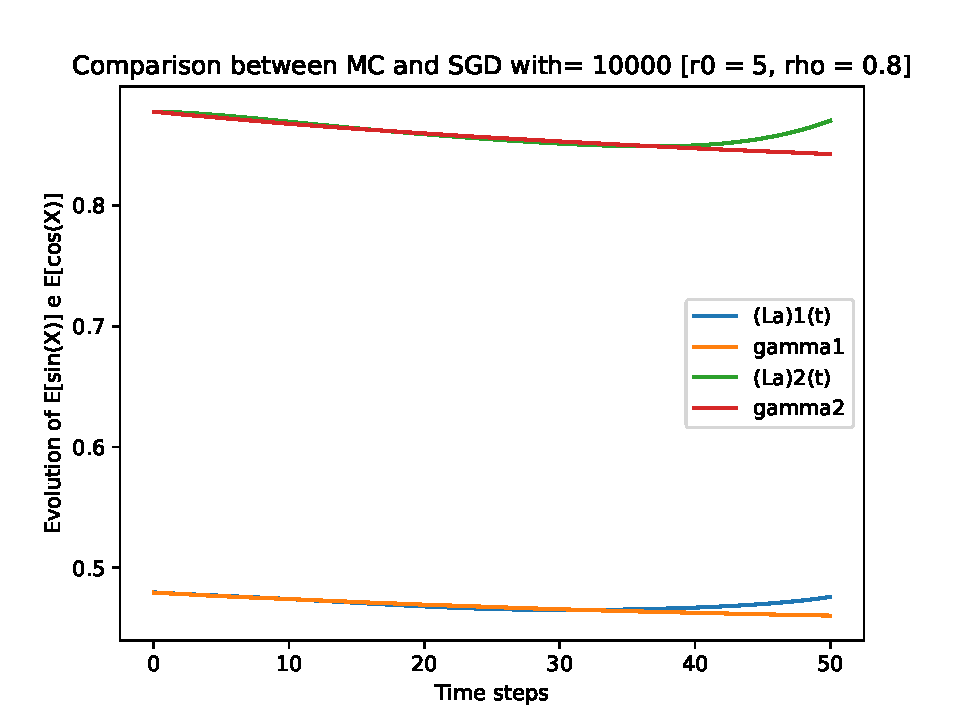
\includegraphics[width=0.9\textwidth]{images/graphs T = 0.5/n = 6, M = 10000 sine and cosine.pdf}
\end{figure}
\newpage
\section{T = 1}
\section*{Case n = 3} 
\begin{table}[H]
\centering
\addtolength{\leftskip}{-1.5cm}
\addtolength{\rightskip}{-1.5cm}
\begin{tabular}{|c|lll|}
\hline
$ $ & $r_0 = 1$ & $r_0 = 5$ & $r_0 = 10$ \\
\hline
$\rho = 0.6$ & 4.60 & 14.19 & 30.59 \\

$\rho = 0.7$ & 6.06 & 8.29 & 13.83 \\

$\rho = 0.8$ & 17.74 & 6.40 & 9.32 \\

$\rho = 0.9$ & 29.5 & 5.47 & 5.58 \\
\hline
\end{tabular}
\caption{Average execution
 times (in seconds $s$) with $M = 1$}
\end{table}
\begin{table}[H]
\centering
\addtolength{\leftskip}{-1.5cm}
\addtolength{\rightskip}{-1.5cm}
\begin{tabular}{|c|lllllllll|}
\hline
$ $ & $r_0 = 1$ & $r_0 = 1$ & $r_0 = 1$ & $r_0 = 5$ & $r_0 = 5$ & $r_0 = 5$ & $r_0 = 10$ & $r_0 = 10$ & $r_0 = 10$  \\
$ $ & min & max & average & min & max & average & min & max & average \\ 
\hline
$\rho = 0.6$ & 220 & 1470 & 683 & 1090 & 3170 & 2090 & 2110 & 6360 & 4544 \\

$\rho = 0.7$ & 170 & 2540 & 921 & 280 & 2290 & 1199 & 890 & 4200 & 2029\\

$\rho = 0.8$ & 160 & 13840 & 2754 & 390 & 1590 & 947 & 580 & 2140 & 1350\\

$\rho = 0.9$ & 690 & 10410 & 4305 & 330 & 1740 & 812 & 230 & 1860 & 836\\
\hline
\end{tabular}
\caption{Number of iterations $m$ to achieve convergence with $M = 1$}
\end{table}
\begin{table}[H]
\centering
\addtolength{\leftskip}{-1.5cm}
\addtolength{\rightskip}{-1.5cm}
\begin{tabular}{|c|lll|}
\hline
$ $ & $r_0 = 1$ & $r_0 = 5$ & $r_0 = 10$ \\
\hline
$\rho = 0.6$ & 1.22 & 1.81 & 3.94 \\

$\rho = 0.7$ & 1.23 & 1.34 & 2.58 \\

$\rho = 0.8$ & 2.29 & 1.33 & 1.53 \\

$\rho = 0.9$ & 6.92 & 0.93 & 1.95 \\
\hline
\end{tabular}
\caption{Average execution
 times (in seconds $s$) with $M = 10$}
\end{table}
\begin{table}[H]
\centering
\addtolength{\leftskip}{-1.5cm}
\addtolength{\rightskip}{-1.5cm}
\begin{tabular}{|c|lllllllll|}
\hline
$ $ & $r_0 = 1$ & $r_0 = 1$ & $r_0 = 1$ & $r_0 = 5$ & $r_0 = 5$ & $r_0 = 5$ & $r_0 = 10$ & $r_0 = 10$ & $r_0 = 10$  \\
$ $ & min & max & average & min & max & average & min & max & average \\ 
\hline
$\rho = 0.6$ & 50 & 330 & 159 & 90 & 440 & 234 & 200 & 1060 & 496 \\

$\rho = 0.7$ & 10 & 500 & 160 & 70 & 500 & 173 & 140 & 500 & 323\\

$\rho = 0.8$ & 30 & 1210 & 298 & 50 & 480 & 172 & 110 & 410 & 194\\

$\rho = 0.9$ & 50 & 2210 & 904 & 50 & 290 & 120 & 20 & 550 & 253\\
\hline
\end{tabular}
\caption{Number of iterations $m$ to achieve convergence with $M = 10$}
\end{table}
\begin{table}[H]
\centering
\addtolength{\leftskip}{-1.5cm}
\addtolength{\rightskip}{-1.5cm}
\begin{tabular}{|c|lll|}
\hline
$ $ & $r_0 = 1$ & $r_0 = 5$ & $r_0 = 10$ \\
\hline
$\rho = 0.6$ & 0.27 & 0.68 & 0.88 \\

$\rho = 0.7$ & 0.39 & 0.47 & 0.92 \\

$\rho = 0.8$ & 0.32 & 0.45 & 0.47 \\

$\rho = 0.9$ & 0.37 & 0.59 &  0.59 \\
\hline
\end{tabular}
\caption{Average execution
 times (in seconds $s$) with $M = 100$}
\end{table}
\begin{table}[H]
\centering
\addtolength{\leftskip}{-1.5cm}
\addtolength{\rightskip}{-1.5cm}
\begin{tabular}{|c|lllllllll|}
\hline
$ $ & $r_0 = 1$ & $r_0 = 1$ & $r_0 = 1$ & $r_0 = 5$ & $r_0 = 5$ & $r_0 = 5$ & $r_0 = 10$ & $r_0 = 10$ & $r_0 = 10$  \\
$ $ & min & max & average & min & max & average & min & max & average \\ 
\hline
$\rho = 0.6$ & 10 & 40 & 21 & 10 & 100 & 54 & 40 & 130 & 69 \\

$\rho = 0.7$ & 10 & 50 & 30 & 10 & 70 & 38 & 20 & 110 & 74\\

$\rho = 0.8$ & 10 & 40 & 25 & 20 & 70 & 36 & 20 & 90 & 38\\

$\rho = 0.9$ & 10 & 50 & 29 & 20 & 150 & 46 & 30 & 90 & 47\\
\hline
\end{tabular}
\caption{Number of iterations $m$ to achieve convergence with $M = 100$}
\end{table}
\begin{table}[H]
\centering
\addtolength{\leftskip}{-1.5cm}
\addtolength{\rightskip}{-1.5cm}
\begin{tabular}{|c|lll|}
\hline
$ $ & $r_0 = 1$ & $r_0 = 5$ & $r_0 = 10$ \\
\hline
$\rho = 0.6$ & 0.49 & 0.62 & 1.82 \\

$\rho = 0.7$ & 0.75 & 0.54 & 1.21 \\

$\rho = 0.8$ & 0.66 & 0.44 & 1.03 \\

$\rho = 0.9$ & 0.82 & 0.46 & 0.75 \\
\hline
\end{tabular}
\caption{Average execution
 times (in seconds $s$) with $M = 1000$}
\end{table}
\begin{table}[H]
\centering
\addtolength{\leftskip}{-1.5cm}
\addtolength{\rightskip}{-1.5cm}
\begin{tabular}{|c|lllllllll|}
\hline
$ $ & $r_0 = 1$ & $r_0 = 1$ & $r_0 = 1$ & $r_0 = 5$ & $r_0 = 5$ & $r_0 = 5$ & $r_0 = 10$ & $r_0 = 10$ & $r_0 = 10$  \\
$ $ & min & max & average & min & max & average & min & max & average \\ 
\hline
$\rho = 0.6$ & 5 & 7 & 5.6 & 6 & 12 & 6.9 & 19 & 24 & 20.8 \\

$\rho = 0.7$ & 5 & 27 & 8.9 & 5 & 9 & 6.3 & 13 & 16 & 14.4 \\

$\rho = 0.8$ & 6 & 10 & 7.9 & 4 & 10 & 5.1 & 10 & 14 & 11.8 \\

$\rho = 0.9$ & 7 & 18 & 9.7 & 4 & 13 & 5.4 & 8 & 13 & 8.9\\
\hline
\end{tabular}
\caption{Number of iterations $m$ to achieve convergence with $M = 1000$}
\end{table}
\begin{table}[H]
\centering
\addtolength{\leftskip}{-1.5cm}
\addtolength{\rightskip}{-1.5cm}
\begin{tabular}{|c|lll|}
\hline
$ $ & $r_0 = 1$ & $r_0 = 5$ & $r_0 = 10$ \\
\hline
$\rho = 0.6$ & 4.71 & 5.83 & 18.25 \\

$\rho = 0.7$ & 5.65 & 4.93 & 12.90 \\

$\rho = 0.8$ & 6.19 & 3.93 & 9.96 \\

$\rho = 0.9$ & 7.45 & 3.98 & 7.93 \\
\hline
\end{tabular}
\caption{Average execution
 times (in seconds $s$) with $M = 10000$}
\end{table}
\begin{table}[H]
\centering
\addtolength{\leftskip}{-1.5cm}
\addtolength{\rightskip}{-1.5cm}
\begin{tabular}{|c|lllllllll|}
\hline
$ $ & $r_0 = 1$ & $r_0 = 1$ & $r_0 = 1$ & $r_0 = 5$ & $r_0 = 5$ & $r_0 = 5$ & $r_0 = 10$ & $r_0 = 10$ & $r_0 = 10$  \\
$ $ & min & max & average & min & max & average & min & max & average \\ 
\hline
$\rho = 0.6$ & 4 & 5 & 4.8 & 6 & 6 & 6 & 17 & 20 & 17.8 \\

$\rho = 0.7$ & 5 & 7 & 5.5 & 5 & 5 & 5 & 13 & 13 & 13\\

$\rho = 0.8$ & 6 & 7 & 6.1 & 4 & 4 & 4 & 10 & 10 & 10\\

$\rho = 0.9$ & 7 & 11 & 7.7 & 4 & 4 & 4 & 8 & 8 & 8\\
\hline
\end{tabular}
\caption{Number of iterations $m$ to achieve convergence with $M = 10000$}
\end{table}
\begin{figure}[H]
\centering
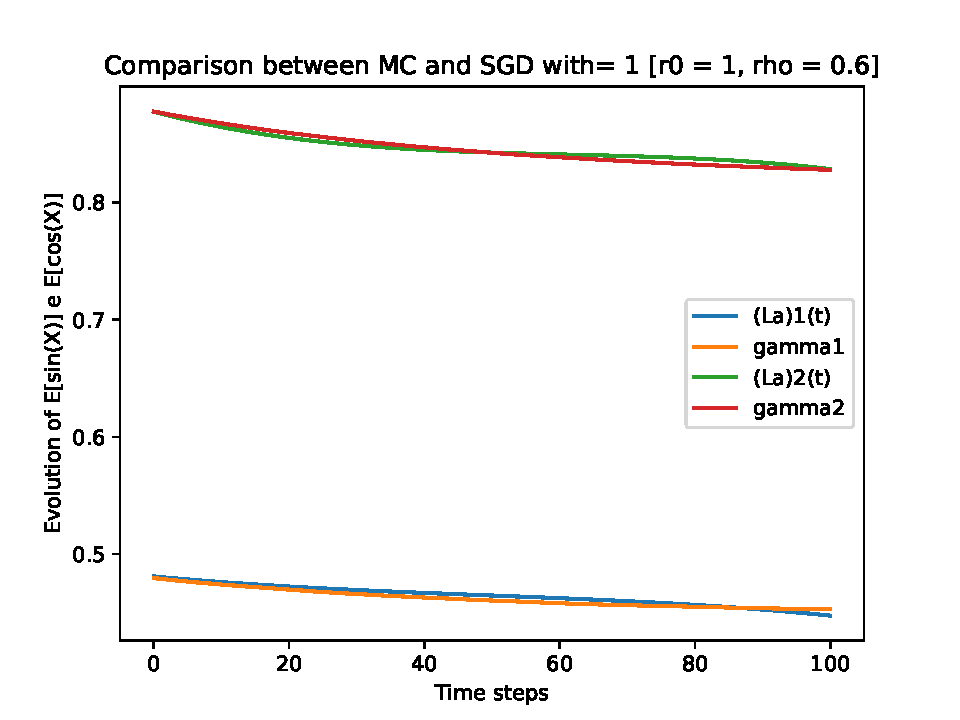
\includegraphics[width=0.9\textwidth]{images/graphs T = 1/n = 3, M = 1 sine and cosine.pdf}
\end{figure}
\begin{figure}[H]
\centering
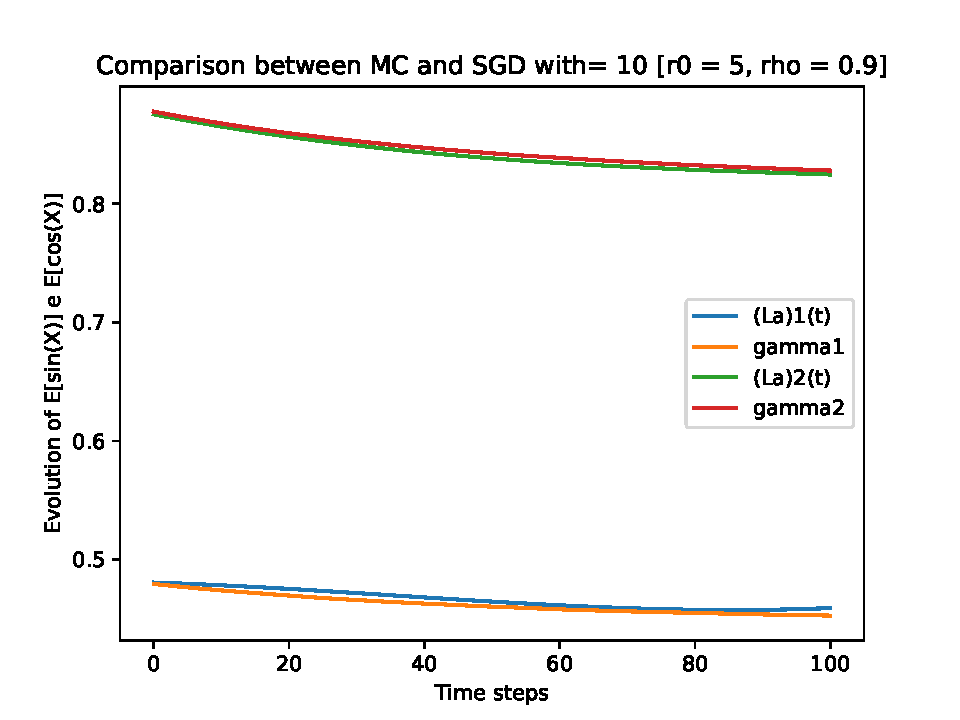
\includegraphics[width=0.9\textwidth]{images/graphs T = 1/n = 3, M = 10 sine and cosine.pdf}
\end{figure}
\begin{figure}[H]
\centering
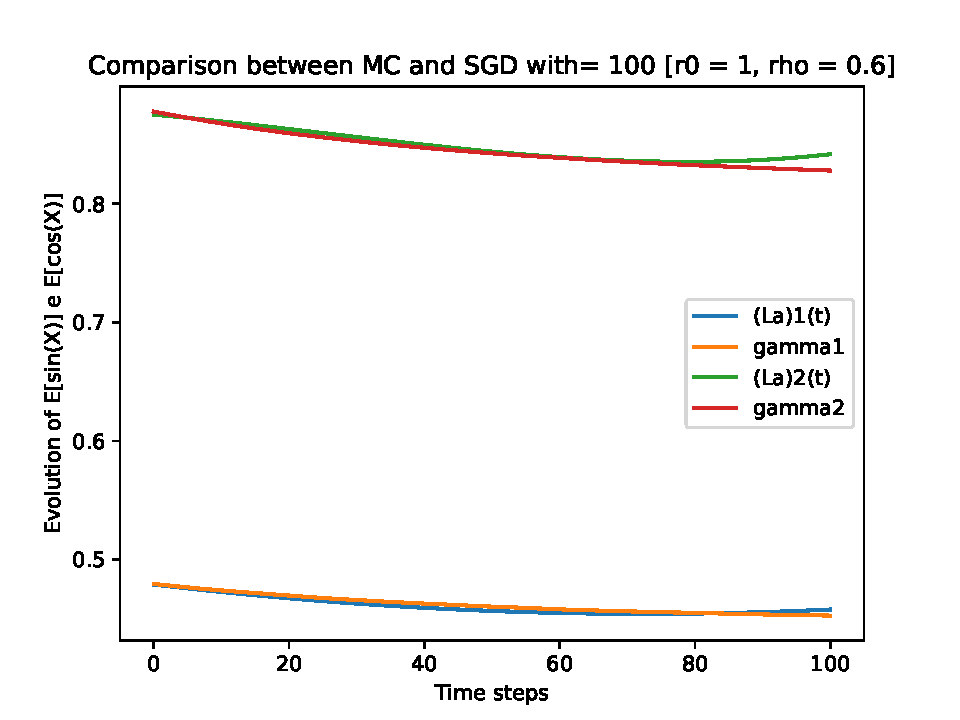
\includegraphics[width=0.9\textwidth]{images/graphs T = 1/n = 3, M = 100 sine and cosine.pdf}
\end{figure}
\begin{figure}[H]
\centering
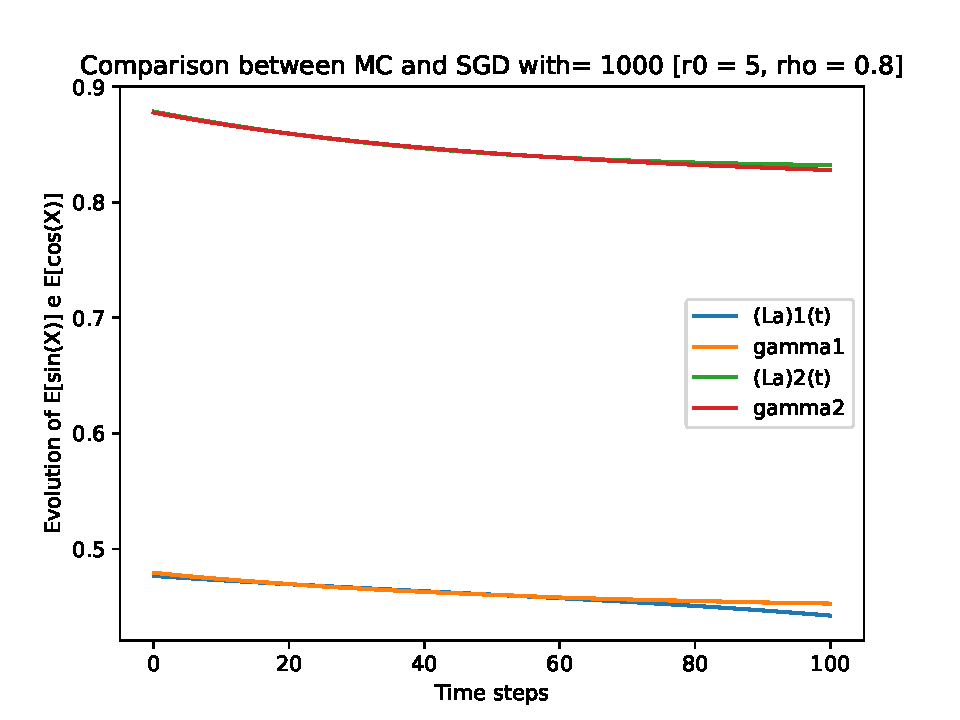
\includegraphics[width=0.9\textwidth]{images/graphs T = 1/n = 3, M = 1000 sine and cosine.pdf}
\end{figure}
\begin{figure}[H]
\centering
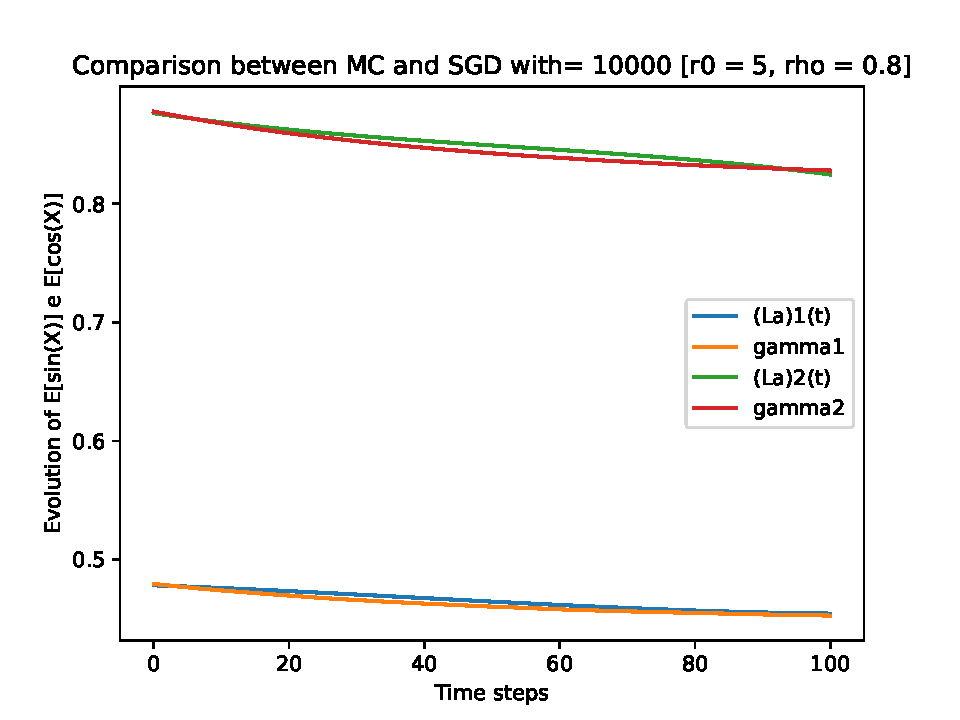
\includegraphics[width=0.9\textwidth]{images/graphs T = 1/n = 3, M = 10000 sine and cosine.pdf}
\end{figure}
\newpage
\section*{Case n = 4} 
\begin{table}[H]
\centering
\addtolength{\leftskip}{-1.5cm}
\addtolength{\rightskip}{-1.5cm}
\begin{tabular}{|c|lll|}
\hline
$ $ & $r_0 = 1$ & $r_0 = 5$ & $r_0 = 10$ \\
\hline
$\rho = 0.6$ & 3.72 & 15.20 & 37.20 \\

$\rho = 0.7$ & 6.40 & 6.31 & 15.76 \\

$\rho = 0.8$ & 10.64 & 5.83 & 9.13 \\

$\rho = 0.9$ & 97.45 & 5.70 & 7.09 \\
\hline
\end{tabular}
\caption{Average execution
 times (in seconds $s$) with $M = 1$}
\end{table}
\begin{table}[H]
\centering
\addtolength{\leftskip}{-1.5cm}
\addtolength{\rightskip}{-1.5cm}
\begin{tabular}{|c|lllllllll|}
\hline
$ $ & $r_0 = 1$ & $r_0 = 1$ & $r_0 = 1$ & $r_0 = 5$ & $r_0 = 5$ & $r_0 = 5$ & $r_0 = 10$ & $r_0 = 10$ & $r_0 = 10$  \\
$ $ & min & max & average & min & max & average & min & max & average \\ 
\hline
$\rho = 0.6$ & 120 & 1280 & 517 & 1080 & 3820 & 2261 & 1830 & 8590 & 5523 \\

$\rho = 0.7$ & 290 & 3140 & 949 & 400 & 1500 & 942 & 540 & 4030 & 2334\\

$\rho = 0.8$ & 170 & 3520 & 1504 & 300 & 1270 & 869 & 440 & 2330 & 1346\\

$\rho = 0.9$ & 720 & 49999 & 14405.8 & 280 & 1960 & 848 & 380 & 1850 & 1047\\
\hline
\end{tabular}
\caption{Number of iterations $m$ to achieve convergence with $M = 1$}
\end{table}
\begin{table}[H]
\centering
\addtolength{\leftskip}{-1.5cm}
\addtolength{\rightskip}{-1.5cm}
\begin{tabular}{|c|lll|}
\hline
$ $ & $r_0 = 1$ & $r_0 = 5$ & $r_0 = 10$ \\
\hline
$\rho = 0.6$ & 0.92 & 2.69 & 6.23 \\

$\rho = 0.7$ & 0.96 & 1.72 & 7.68 \\

$\rho = 0.8$ & 2.55 & 1.45 & 5.01 \\

$\rho = 0.9$ & 17.99 & 1.39 & 3.59 \\
\hline
\end{tabular}
\caption{Average execution
 times (in seconds $s$) with $M = 10$}
\end{table}
\begin{table}[H]
\centering
\addtolength{\leftskip}{-1.5cm}
\addtolength{\rightskip}{-1.5cm}
\begin{tabular}{|c|lllllllll|}
\hline
$ $ & $r_0 = 1$ & $r_0 = 1$ & $r_0 = 1$ & $r_0 = 5$ & $r_0 = 5$ & $r_0 = 5$ & $r_0 = 10$ & $r_0 = 10$ & $r_0 = 10$  \\
$ $ & min & max & average & min & max & average & min & max & average \\ 
\hline
$\rho = 0.6$ & 50 & 180 & 117 & 110 & 590 & 340 & 260 & 890 & 548 \\

$\rho = 0.7$ & 10 & 300 & 123 & 100 & 660 & 219 & 190 & 530 & 369\\

$\rho = 0.8$ & 40 & 910 & 325 & 70 & 290 & 183 & 100 & 450 & 256\\

$\rho = 0.9$ & 40 & 11880 & 2280 & 20 & 520 & 177 & 60 & 310 & 180\\
\hline
\end{tabular}
\caption{Number of iterations $m$ to achieve convergence with $M = 10$}
\end{table}
\begin{table}[H]
\centering
\addtolength{\leftskip}{-1.5cm}
\addtolength{\rightskip}{-1.5cm}
\begin{tabular}{|c|lll|}
\hline
$ $ & $r_0 = 1$ & $r_0 = 5$ & $r_0 = 10$ \\
\hline
$\rho = 0.6$ & 1.36 & 2.10 & 3.85 \\

$\rho = 0.7$ & 1.81 & 1.36 & 2.15 \\

$\rho = 0.8$ & 1.61 & 1.74 & 1.55 \\

$\rho = 0.9$ & 1.33 & 1.11 & 1.45 \\
\hline
\end{tabular}
\caption{Average execution
 times (in seconds $s$) with $M = 100$}
\end{table}
\begin{table}[H]
\centering
\addtolength{\leftskip}{-1.5cm}
\addtolength{\rightskip}{-1.5cm}
\begin{tabular}{|c|lllllllll|}
\hline
$ $ & $r_0 = 1$ & $r_0 = 1$ & $r_0 = 1$ & $r_0 = 5$ & $r_0 = 5$ & $r_0 = 5$ & $r_0 = 10$ & $r_0 = 10$ & $r_0 = 10$  \\
$ $ & min & max & average & min & max & average & min & max & average \\ 
\hline
$\rho = 0.6$ & 10 & 130 & 40 & 20 & 150 & 62 & 60 & 140 & 106 \\

$\rho = 0.7$ & 20 & 260 & 55 & 10 & 100 & 39 & 20 & 150 & 61\\

$\rho = 0.8$ & 20 & 80 & 49 & 20 & 80 & 48 & 20 & 90 & 44\\

$\rho = 0.9$ & 10 & 120 & 41 & 10 & 60 & 31 & 20 & 60 & 41\\
\hline
\end{tabular}
\caption{Number of iterations $m$ to achieve convergence with $M = 100$}
\end{table}
\begin{table}[H]
\centering
\addtolength{\leftskip}{-1.5cm}
\addtolength{\rightskip}{-1.5cm}
\begin{tabular}{|c|lll|}
\hline
$ $ & $r_0 = 1$ & $r_0 = 5$ & $r_0 = 10$ \\
\hline
$\rho = 0.6$ & 2.17 & 1.38 & 3.64 \\

$\rho = 0.7$ & 2.24 & 1.33 & 2.73 \\

$\rho = 0.8$ & 3.97 & 1.31 & 2.31 \\

$\rho = 0.9$ & 5.90 & 1.08 & 1.85 \\
\hline
\end{tabular}
\caption{Average execution
 times (in seconds $s$) with $M = 1000$}
\end{table}
\begin{table}[H]
\centering
\addtolength{\leftskip}{-1.5cm}
\addtolength{\rightskip}{-1.5cm}
\begin{tabular}{|c|lllllllll|}
\hline
$ $ & $r_0 = 1$ & $r_0 = 1$ & $r_0 = 1$ & $r_0 = 5$ & $r_0 = 5$ & $r_0 = 5$ & $r_0 = 10$ & $r_0 = 10$ & $r_0 = 10$  \\
$ $ & min & max & average & min & max & average & min & max & average \\ 
\hline
$\rho = 0.6$ & 7 & 12 & 9.1 & 4 & 10 & 5.9 & 13 & 21 & 15.3 \\

$\rho = 0.7$ & 8 & 16 & 9.5 & 4 & 13 & 5.6 & 10 & 15 & 11.5 \\

$\rho = 0.8$ & 10 & 40 & 16.2 & 3 & 11 & 5.6 & 8 & 15 & 9.8 \\

$\rho = 0.9$ & 12 & 58 & 24.7 & 3 & 11 & 4.6 & 7 & 11 & 7.9\\
\hline
\end{tabular}
\caption{Number of iterations $m$ to achieve convergence with $M = 1000$}
\end{table}
\begin{table}[H]
\centering
\addtolength{\leftskip}{-1.5cm}
\addtolength{\rightskip}{-1.5cm}
\begin{tabular}{|c|lll|}
\hline
$ $ & $r_0 = 1$ & $r_0 = 5$ & $r_0 = 10$ \\
\hline
$\rho = 0.6$ & 17.09 & 10.90 & 33.12 \\

$\rho = 0.7$ & 20.29 & 9.95 & 24.45 \\

$\rho = 0.8$ & 25.10 & 9.10 & 16.95 \\

$\rho = 0.9$ & 32.85 & 8.00 & 7.84 \\
\hline
\end{tabular}
\caption{Average execution
 times (in seconds $s$) with $M = 10000$}
\end{table}
\begin{table}[H]
\centering
\addtolength{\leftskip}{-1.5cm}
\addtolength{\rightskip}{-1.5cm}
\begin{tabular}{|c|lllllllll|}
\hline
$ $ & $r_0 = 1$ & $r_0 = 1$ & $r_0 = 1$ & $r_0 = 5$ & $r_0 = 5$ & $r_0 = 5$ & $r_0 = 10$ & $r_0 = 10$ & $r_0 = 10$  \\
$ $ & min & max & average & min & max & average & min & max & average \\ 
\hline
$\rho = 0.6$ & 7 & 7 & 7 & 4 & 5 & 4.4 & 13 & 14 & 13.3 \\

$\rho = 0.7$ & 7 & 9 & 8.3 & 4 & 4 & 4 & 10 & 10 & 10\\

$\rho = 0.8$ & 9 & 13 & 10.2 & 3 & 4 & 3.7 & 8 & 8 & 8\\

$\rho = 0.9$ & 12 & 15 & 13.3 & 3 & 3 & 3 & 7 & 7 & 7\\
\hline
\end{tabular}
\caption{Number of iterations $m$ to achieve convergence with $M = 10000$}
\end{table}
\begin{figure}[H]
\centering
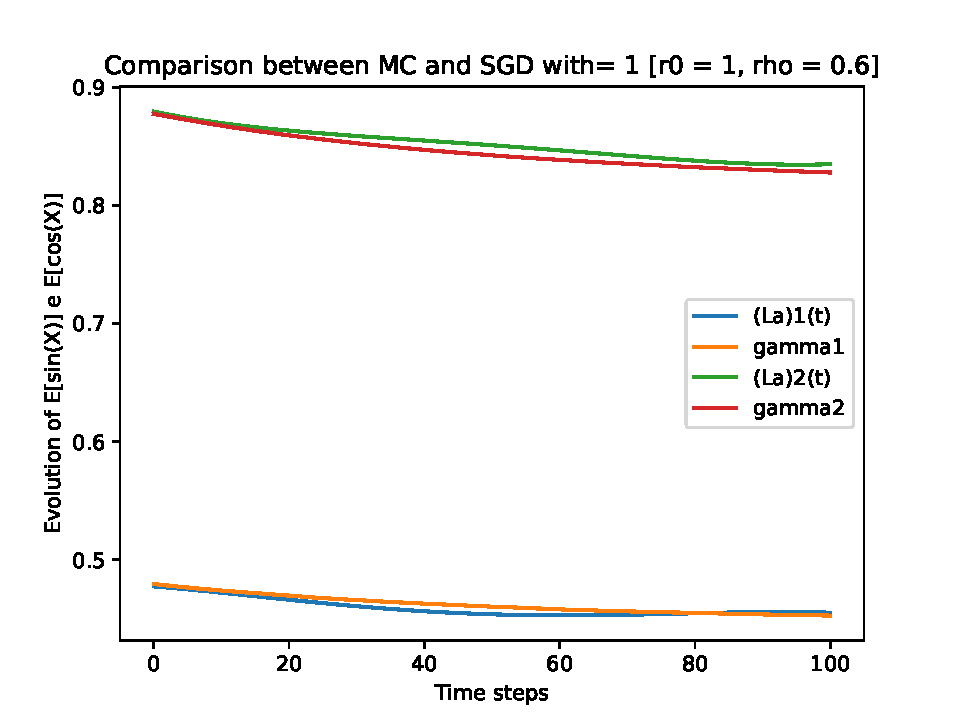
\includegraphics[width=0.9\textwidth]{images/graphs T = 1/n = 4, M = 1 sine and cosine.pdf}
\end{figure}
\begin{figure}[H]
\centering
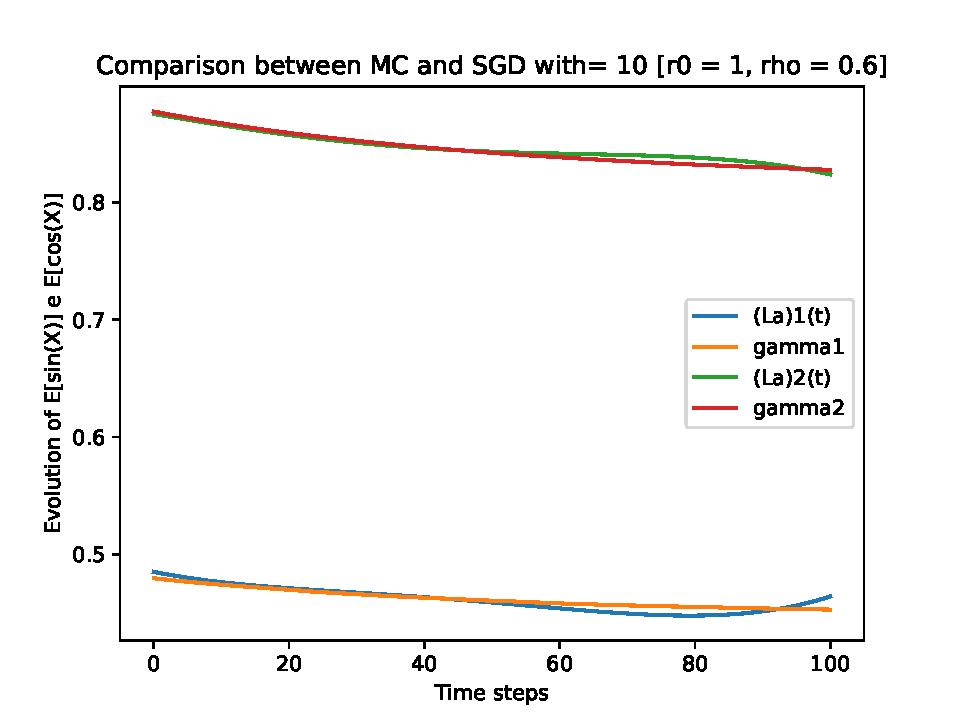
\includegraphics[width=0.9\textwidth]{images/graphs T = 1/n = 4, M = 10 sine and cosine.pdf}
\end{figure}
\begin{figure}[H]
\centering
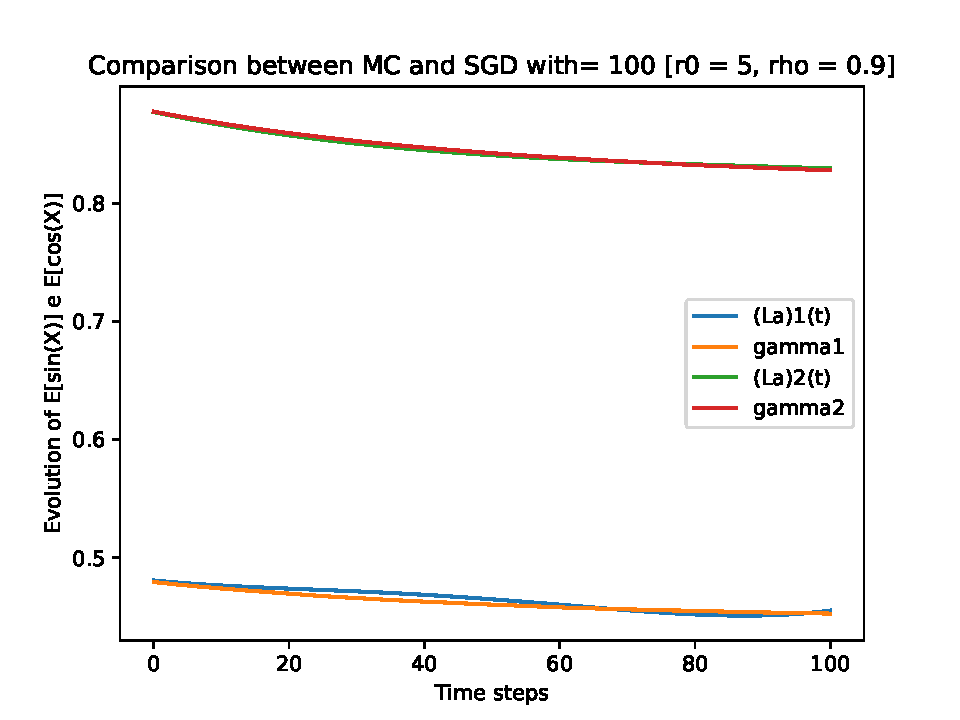
\includegraphics[width=0.9\textwidth]{images/graphs T = 1/n = 4, M = 100 sine and cosine.pdf}
\end{figure}
\begin{figure}[H]
\centering
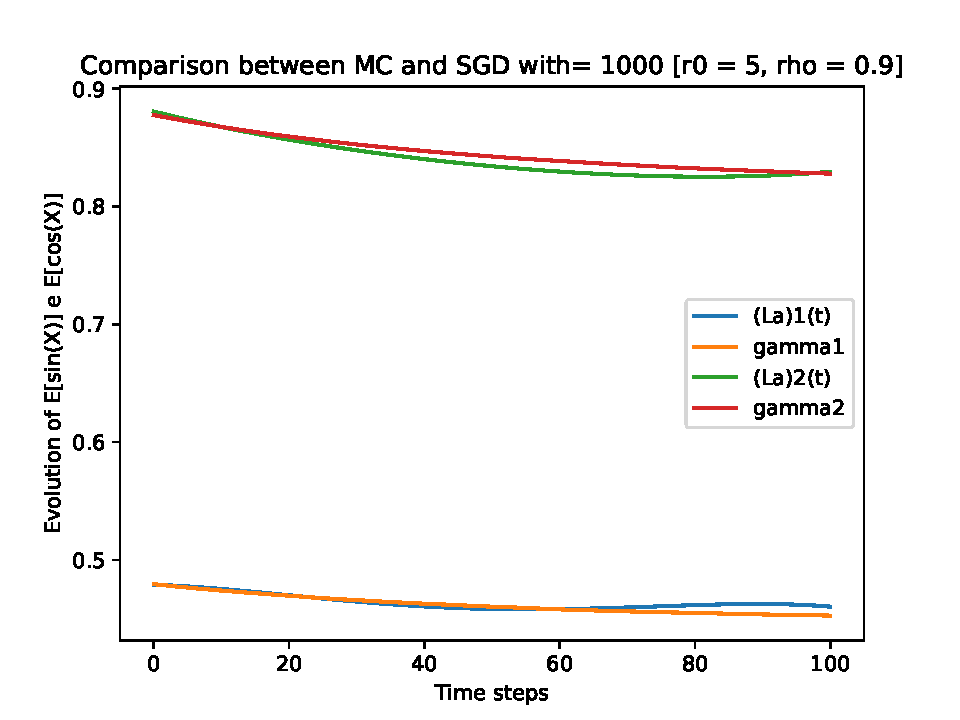
\includegraphics[width=0.9\textwidth]{images/graphs T = 1/n = 4, M = 1000 sine and cosine.pdf}
\end{figure}
\begin{figure}[H]
\centering
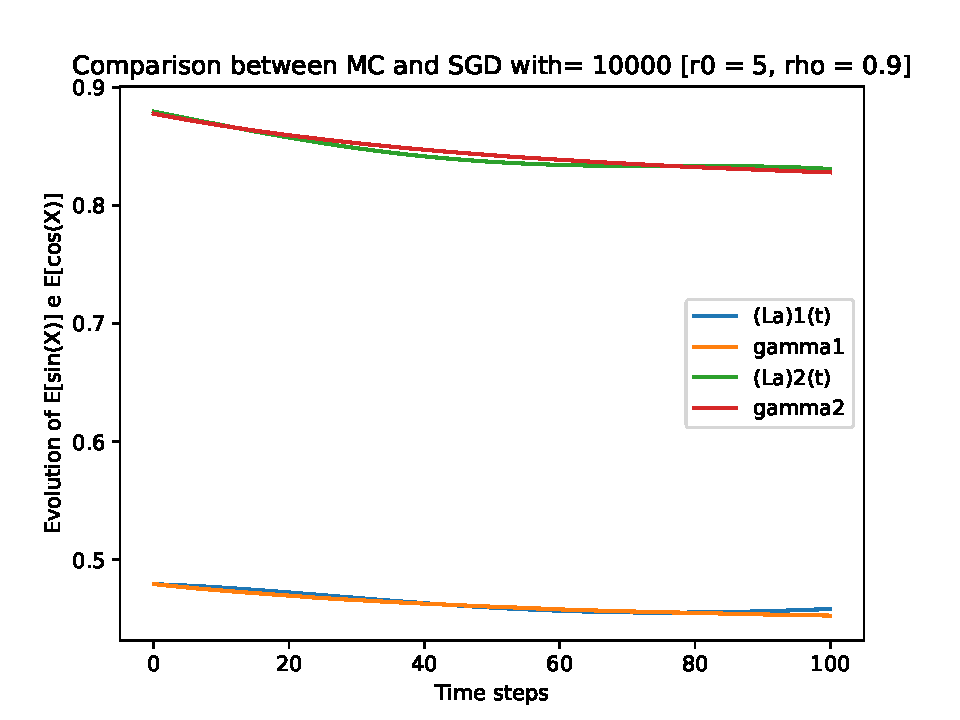
\includegraphics[width=0.9\textwidth]{images/graphs T = 1/n = 4, M = 10000 sine and cosine.pdf}
\end{figure}
\newpage
\section*{Case n = 5} 
\begin{table}[H]
\centering
\addtolength{\leftskip}{-1.5cm}
\addtolength{\rightskip}{-1.5cm}
\begin{tabular}{|c|lll|}
\hline
$ $ & $r_0 = 1$ & $r_0 = 5$ & $r_0 = 10$ \\
\hline
$\rho = 0.6$ & 4.81 & 14.76 & 31.03 \\

$\rho = 0.7$ & 9.11 & 7.29 & 17.28 \\

$\rho = 0.8$ & 31.30 & 5.37 & 10.54 \\

$\rho = 0.9$ & 90.16 & 6.65 & 5.83 \\
\hline
\end{tabular}
\caption{Average execution
 times (in seconds $s$) with $M = 1$}
\end{table}
\begin{table}[H]
\centering
\addtolength{\leftskip}{-1.5cm}
\addtolength{\rightskip}{-1.5cm}
\begin{tabular}{|c|lllllllll|}
\hline
$ $ & $r_0 = 1$ & $r_0 = 1$ & $r_0 = 1$ & $r_0 = 5$ & $r_0 = 5$ & $r_0 = 5$ & $r_0 = 10$ & $r_0 = 10$ & $r_0 = 10$  \\
$ $ & min & max & average & min & max & average & min & max & average \\ 
\hline
$\rho = 0.6$ & 340 & 1340 & 709 & 1670 & 3170 & 2166 & 1690 & 8820 & 4546 \\

$\rho = 0.7$ & 410 & 2260 & 1323 & 160 & 2300 & 1071 & 770 & 4350 & 2533\\

$\rho = 0.8$ & 240 & 24910 & 4579 & 90 & 1650 & 789 & 820 & 2910 & 1543\\

$\rho = 0.9$ & 570 & 49999 & 13249.9 & 470 & 1860 & 978 & 380 & 1350 & 857\\
\hline
\end{tabular}
\caption{Number of iterations $m$ to achieve convergence with $M = 1$}
\end{table}
\begin{table}[H]
\centering
\addtolength{\leftskip}{-1.5cm}
\addtolength{\rightskip}{-1.5cm}
\begin{tabular}{|c|lll|}
\hline
$ $ & $r_0 = 1$ & $r_0 = 5$ & $r_0 = 10$ \\
\hline
$\rho = 0.6$ & 1.42 & 1.65 & 4.35 \\

$\rho = 0.7$ & 1.71 & 1.87 &  2.07 \\

$\rho = 0.8$ & 3.27 & 1.42 & 1.88 \\

$\rho = 0.9$ & 1.47 & 1.26 & 1.81 \\
\hline
\end{tabular}
\caption{Average execution
 times (in seconds $s$) with $M = 10$}
\end{table}
\begin{table}[H]
\centering
\addtolength{\leftskip}{-1.5cm}
\addtolength{\rightskip}{-1.5cm}
\begin{tabular}{|c|lllllllll|}
\hline
$ $ & $r_0 = 1$ & $r_0 = 1$ & $r_0 = 1$ & $r_0 = 5$ & $r_0 = 5$ & $r_0 = 5$ & $r_0 = 10$ & $r_0 = 10$ & $r_0 = 10$  \\
$ $ & min & max & average & min & max & average & min & max & average \\ 
\hline
$\rho = 0.6$ & 50 & 580 & 179 & 80 & 420 & 206 & 120 & 870 & 540 \\

$\rho = 0.7$ & 60 & 1180 & 216 & 80 & 430 & 235 & 120 & 570 & 257\\

$\rho = 0.8$ & 50 & 1460 & 411 & 140 & 330 & 178 & 70 & 390 & 235\\

$\rho = 0.9$ & 40 & 750 & 185 & 50 & 370 & 157 & 90 & 490 & 228\\
\hline
\end{tabular}
\caption{Number of iterations $m$ to achieve convergence with $M = 10$}
\end{table}
\begin{table}[H]
\centering
\addtolength{\leftskip}{-1.5cm}
\addtolength{\rightskip}{-1.5cm}
\begin{tabular}{|c|lll|}
\hline
$ $ & $r_0 = 1$ & $r_0 = 5$ & $r_0 = 10$ \\
\hline
$\rho = 0.6$ & 0.66 & 0.47 & 1.23 \\

$\rho = 0.7$ & 0.63 & 0.69 & 0.87 \\

$\rho = 0.8$ & 0.73 & 0.39 & 0.95 \\

$\rho = 0.9$ & 1.93 & 0.49 & 0.43 \\
\hline
\end{tabular}
\caption{Average execution
 times (in seconds $s$) with $M = 100$}
\end{table}
\begin{table}[H]
\centering
\addtolength{\leftskip}{-1.5cm}
\addtolength{\rightskip}{-1.5cm}
\begin{tabular}{|c|lllllllll|}
\hline
$ $ & $r_0 = 1$ & $r_0 = 1$ & $r_0 = 1$ & $r_0 = 5$ & $r_0 = 5$ & $r_0 = 5$ & $r_0 = 10$ & $r_0 = 10$ & $r_0 = 10$  \\
$ $ & min & max & average & min & max & average & min & max & average \\ 
\hline
$\rho = 0.6$ & 20 & 100 & 46 & 10 & 60 & 33 & 30 & 150 & 86 \\

$\rho = 0.7$ & 20 & 150 & 44 & 10 & 130 & 48 & 20 & 90 & 61\\

$\rho = 0.8$ & 20 & 180 & 51 & 10 & 40 & 27 & 30 & 110 & 66\\

$\rho = 0.9$ & 40 & 370 & 135 & 10 & 90 & 34 & 10 & 60 & 30\\
\hline
\end{tabular}
\caption{Number of iterations $m$ to achieve convergence with $M = 100$}
\end{table}
\begin{table}[H]
\centering
\addtolength{\leftskip}{-1.5cm}
\addtolength{\rightskip}{-1.5cm}
\begin{tabular}{|c|lll|}
\hline
$ $ & $r_0 = 1$ & $r_0 = 5$ & $r_0 = 10$ \\
\hline
$\rho = 0.6$ & 1.35 & 0.67 & 1.37 \\

$\rho = 0.7$ & 1.48 & 0.52 & 0.92 \\

$\rho = 0.8$ & 2.33 & 0.37 & 0.87 \\

$\rho = 0.9$ & 3.61 & 0.53 & 0.74 \\
\hline
\end{tabular}
\caption{Average execution
 times (in seconds $s$) with $M = 1000$}
\end{table}
\begin{table}[H]
\centering
\addtolength{\leftskip}{-1.5cm}
\addtolength{\rightskip}{-1.5cm}
\begin{tabular}{|c|lllllllll|}
\hline
$ $ & $r_0 = 1$ & $r_0 = 1$ & $r_0 = 1$ & $r_0 = 5$ & $r_0 = 5$ & $r_0 = 5$ & $r_0 = 10$ & $r_0 = 10$ & $r_0 = 10$  \\
$ $ & min & max & average & min & max & average & min & max & average \\ 
\hline
$\rho = 0.6$ & 10 & 18 & 12.3 & 3 & 14 & 6.1 & 10 & 15 & 12.5 \\

$\rho = 0.7$ & 11 & 16 & 13.4 & 3 & 8 & 4.7 & 8 & 10 & 8.4 \\

$\rho = 0.8$ & 17 & 27 & 21.1 & 3 & 4 & 3.3 & 6 & 12 & 7.9 \\

$\rho = 0.9$ & 23 & 66 & 32.9 & 3 & 11 & 4.8 & 6 & 8 & 6.7\\
\hline
\end{tabular}
\caption{Number of iterations $m$ to achieve convergence with $M = 1000$}
\end{table}
\begin{table}[H]
\centering
\addtolength{\leftskip}{-1.5cm}
\addtolength{\rightskip}{-1.5cm}
\begin{tabular}{|c|lll|}
\hline
$ $ & $r_0 = 1$ & $r_0 = 5$ & $r_0 = 10$ \\
\hline
$\rho = 0.6$ & 13.12 & 4.45 & 13.18 \\

$\rho = 0.7$ & 15.57 & 3.89 & 10.47 \\

$\rho = 0.8$ & 20.77 & 3.93 & 8.27 \\

$\rho = 0.9$ & 31.73 & 3.90 & 7.20 \\
\hline
\end{tabular}
\caption{Average execution
 times (in seconds $s$) with $M = 10000$}
\end{table}
\begin{table}[H]
\centering
\addtolength{\leftskip}{-1.5cm}
\addtolength{\rightskip}{-1.5cm}
\begin{tabular}{|c|lllllllll|}
\hline
$ $ & $r_0 = 1$ & $r_0 = 1$ & $r_0 = 1$ & $r_0 = 5$ & $r_0 = 5$ & $r_0 = 5$ & $r_0 = 10$ & $r_0 = 10$ & $r_0 = 10$  \\
$ $ & min & max & average & min & max & average & min & max & average \\ 
\hline
$\rho = 0.6$ & 9 & 11 & 10 & 3 & 4 & 3.4 & 10 & 11 & 10.1 \\

$\rho = 0.7$ & 11 & 13 & 11.9 & 3 & 3 & 3 & 8 & 8 & 8\\

$\rho = 0.8$ & 15 & 16 & 15.9 & 3 & 3 & 3 & 6 & 7 & 6.3\\

$\rho = 0.9$ & 22 & 31 & 24.3 & 3 & 3 & 3 & 5 & 6 & 5.5\\
\hline
\end{tabular}
\caption{Number of iterations $m$ to achieve convergence with $M = 10000$}
\end{table}
\begin{figure}[H]
\centering
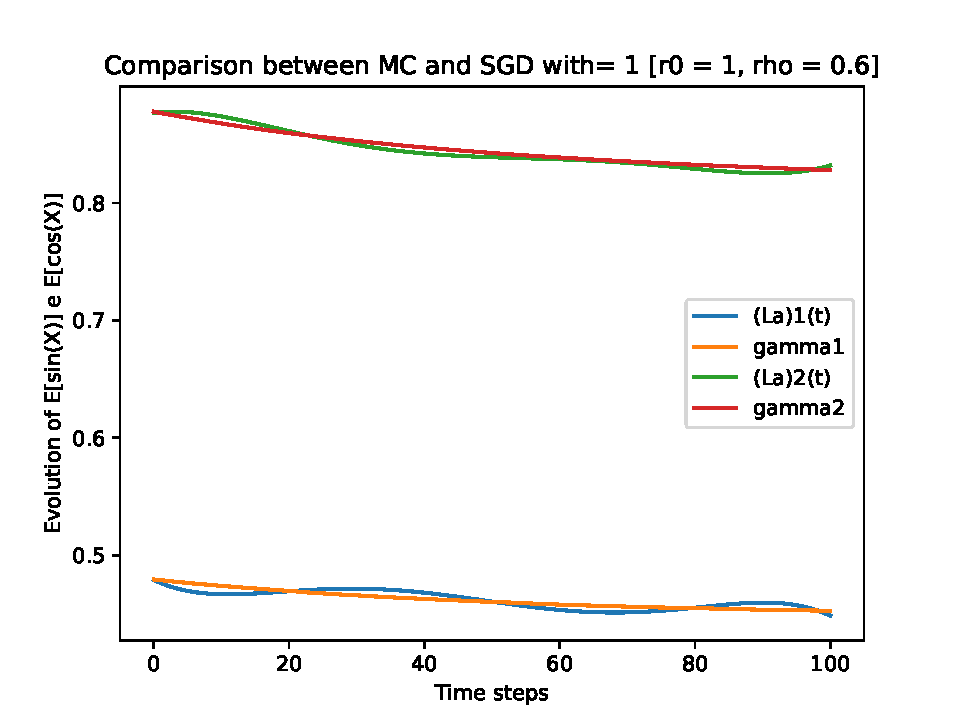
\includegraphics[width=0.9\textwidth]{images/graphs T = 1/n = 5, M = 1 sine and cosine.pdf}
\end{figure}
\begin{figure}[H]
\centering
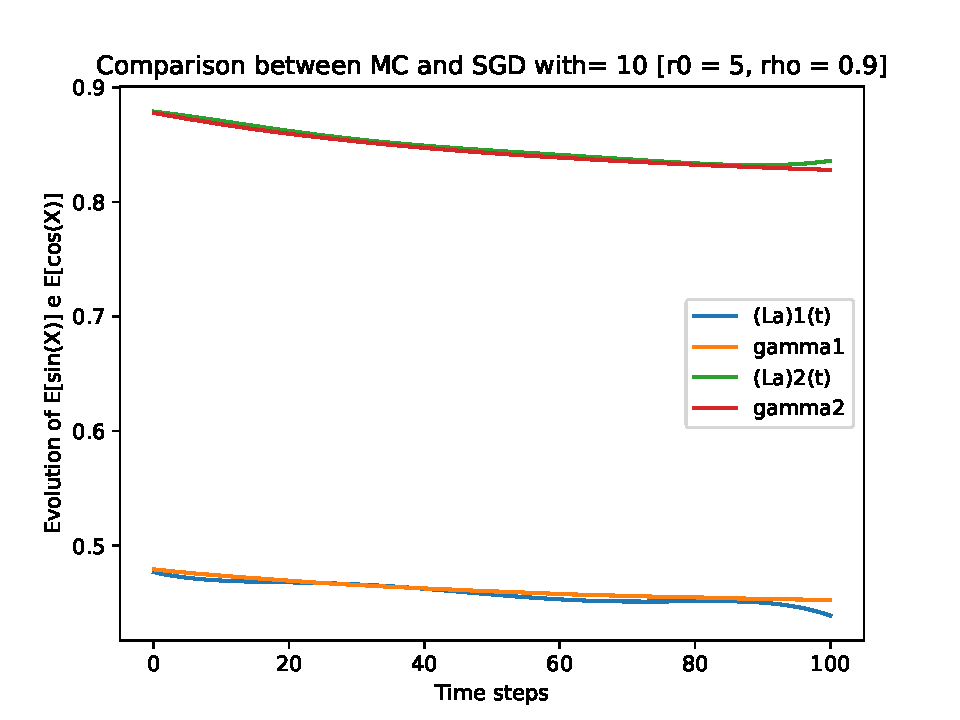
\includegraphics[width=0.9\textwidth]{images/graphs T = 1/n = 5, M = 10 sine and cosine.pdf}
\end{figure}
\begin{figure}[H]
\centering
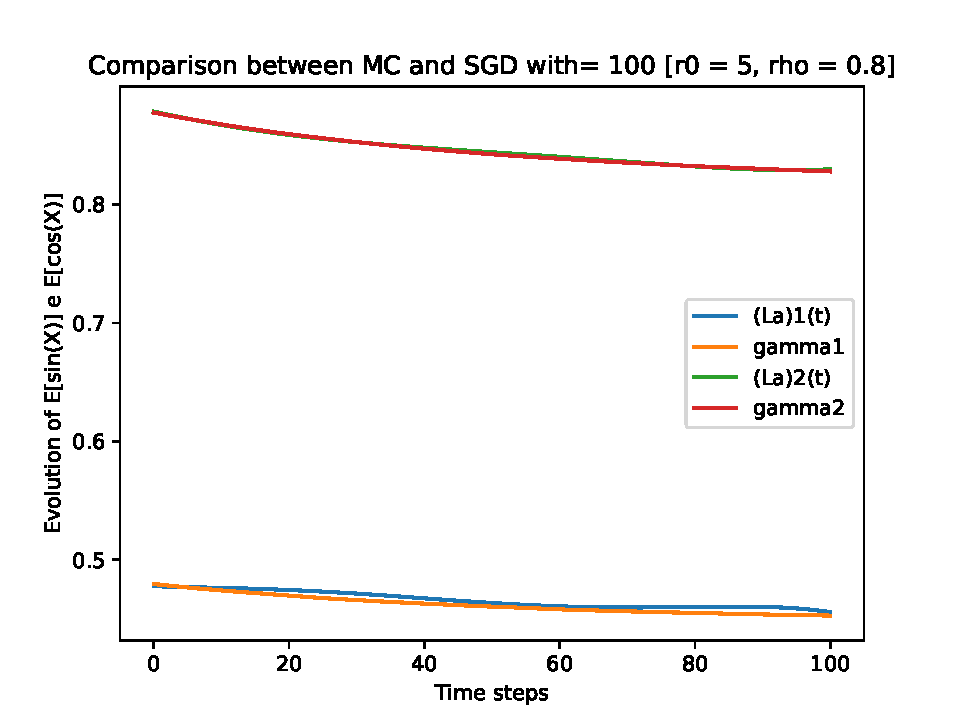
\includegraphics[width=0.9\textwidth]{images/graphs T = 1/n = 5, M = 100 sine and cosine.pdf}
\end{figure}
\begin{figure}[H]
\centering
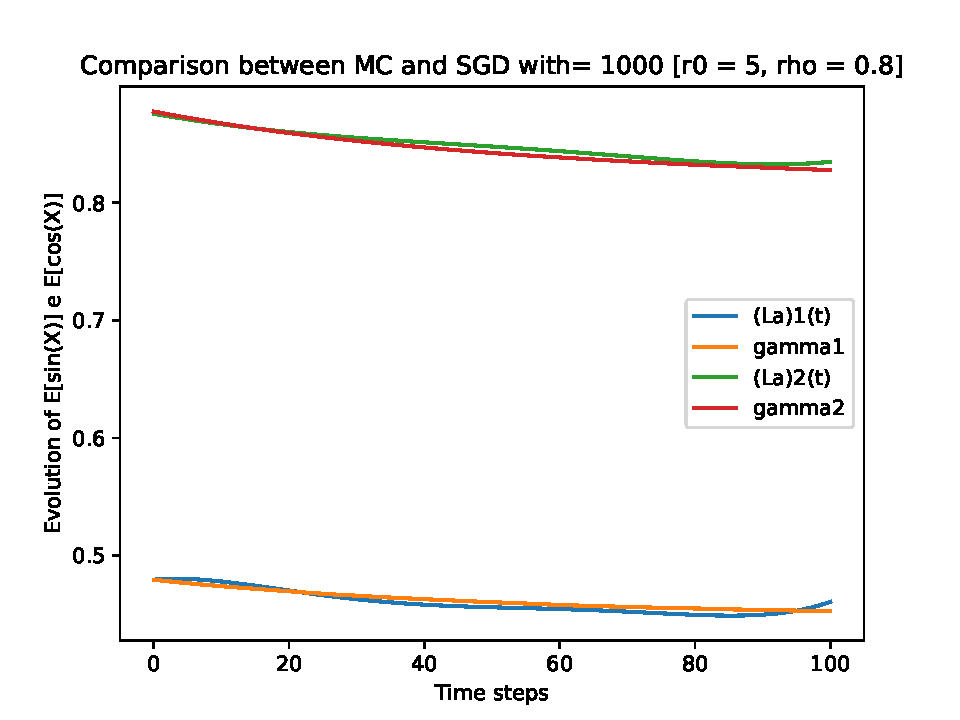
\includegraphics[width=0.9\textwidth]{images/graphs T = 1/n = 5, M = 1000 sine and cosine.pdf}
\end{figure}
\begin{figure}[H]
\centering
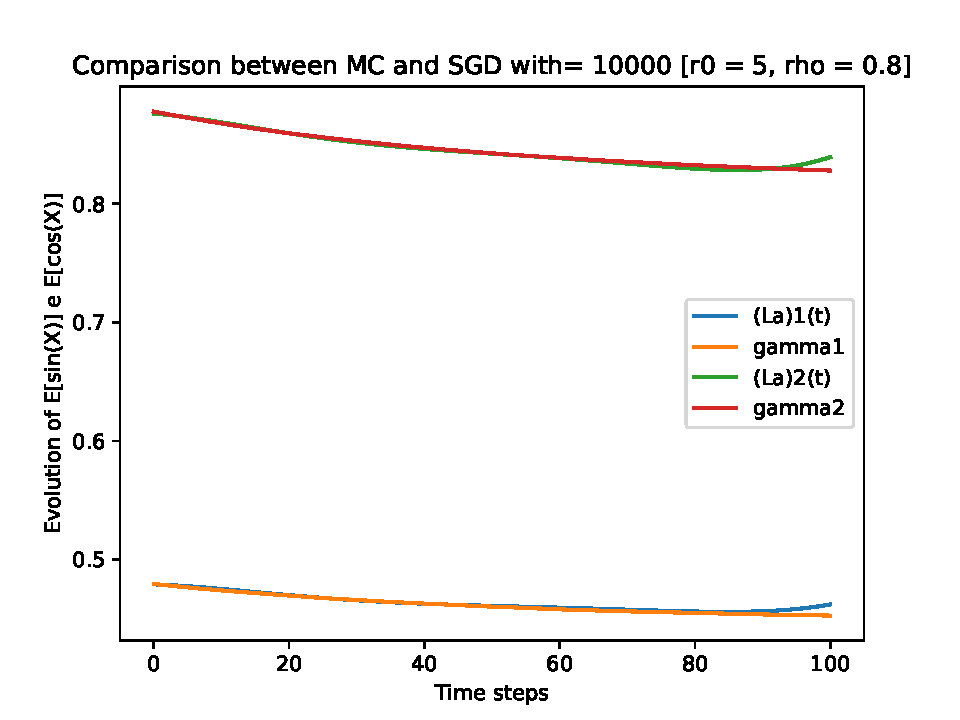
\includegraphics[width=0.9\textwidth]{images/graphs T = 1/n = 5, M = 10000 sine and cosine.pdf}
\end{figure}
\newpage
\section*{Case n = 6} 
\begin{table}[H]
\centering
\addtolength{\leftskip}{-1.5cm}
\addtolength{\rightskip}{-1.5cm}
\begin{tabular}{|c|lll|}
\hline
$ $ & $r_0 = 1$ & $r_0 = 5$ & $r_0 = 10$ \\
\hline
$\rho = 0.6$ & 7.97 & 13.95 & 35.22 \\

$\rho = 0.7$ & 11.89 & 9.05 & 18.96 \\

$\rho = 0.8$ & 17.13 & 10.48 & 9.50 \\

$\rho = 0.9$ & 157.41 & 10.32 & 6.82 \\
\hline
\end{tabular}
\caption{Average execution
 times (in seconds $s$) with $M = 1$}
\end{table}
\begin{table}[H]
\centering
\addtolength{\leftskip}{-1.5cm}
\addtolength{\rightskip}{-1.5cm}
\begin{tabular}{|c|lllllllll|}
\hline
$ $ & $r_0 = 1$ & $r_0 = 1$ & $r_0 = 1$ & $r_0 = 5$ & $r_0 = 5$ & $r_0 = 5$ & $r_0 = 10$ & $r_0 = 10$ & $r_0 = 10$  \\
$ $ & min & max & average & min & max & average & min & max & average \\ 
\hline
$\rho = 0.6$ & 170 & 1920 & 1142 & 610 & 3310 & 1991 & 2510 & 9890 & 5037 \\

$\rho = 0.7$ & 320 & 6730 & 1702 & 210 & 2550 & 1292 & 770 & 3790 & 2713\\

$\rho = 0.8$ & 390 & 10610 & 2453 & 500 & 3180 & 1501 & 540 & 2200 & 1359\\

$\rho = 0.9$ & 590 & 49999 & 22514.8 & 430 & 5640 & 1475 & 380 & 2510 & 976\\
\hline
\end{tabular}
\caption{Number of iterations $m$ to achieve convergence with $M = 1$}
\end{table}
\begin{table}[H]
\centering
\addtolength{\leftskip}{-1.5cm}
\addtolength{\rightskip}{-1.5cm}
\begin{tabular}{|c|lll|}
\hline
$ $ & $r_0 = 1$ & $r_0 = 5$ & $r_0 = 10$ \\
\hline
$\rho = 0.6$ & 1.13 & 2.55 & 6.69 \\

$\rho = 0.7$ & 2.00 & 2.10 & 4.14 \\

$\rho = 0.8$ & 5.07 & 2.23 & 2.89 \\

$\rho = 0.9$ & 19.58 & 1.94 & 2.00 \\
\hline
\end{tabular}
\caption{Average execution
 times (in seconds $s$) with $M = 10$}
\end{table}
\begin{table}[H]
\centering
\addtolength{\leftskip}{-1.5cm}
\addtolength{\rightskip}{-1.5cm}
\begin{tabular}{|c|lllllllll|}
\hline
$ $ & $r_0 = 1$ & $r_0 = 1$ & $r_0 = 1$ & $r_0 = 5$ & $r_0 = 5$ & $r_0 = 5$ & $r_0 = 10$ & $r_0 = 10$ & $r_0 = 10$  \\
$ $ & min & max & average & min & max & average & min & max & average \\ 
\hline
$\rho = 0.6$ & 40 & 220 & 96 & 100 & 420 & 216 & 230 & 880 & 565 \\

$\rho = 0.7$ & 30 & 430 & 171 & 70 & 330 & 178 & 130 & 580 & 351\\

$\rho = 0.8$ & 40 & 1560 & 431 & 70 & 550 & 187 & 70 & 360 & 246\\

$\rho = 0.9$ & 100 & 6200 & 1661 & 60 & 270 & 164 & 70 & 330 & 170\\
\hline
\end{tabular}
\caption{Number of iterations $m$ to achieve convergence with $M = 10$}
\end{table}
\begin{table}[H]
\centering
\addtolength{\leftskip}{-1.5cm}
\addtolength{\rightskip}{-1.5cm}
\begin{tabular}{|c|lll|}
\hline
$ $ & $r_0 = 1$ & $r_0 = 5$ & $r_0 = 10$ \\
\hline
$\rho = 0.6$ & 0.62 & 0.72 & 1.11 \\

$\rho = 0.7$ & 0.86 & 0.52 & 0.85 \\

$\rho = 0.8$ & 1.57 & 0.34 & 0.73 \\

$\rho = 0.9$ & 1.55 & 0.54 & 0.46 \\
\hline
\end{tabular}
\caption{Average execution
 times (in seconds $s$) with $M = 100$}
\end{table}
\begin{table}[H]
\centering
\addtolength{\leftskip}{-1.5cm}
\addtolength{\rightskip}{-1.5cm}
\begin{tabular}{|c|lllllllll|}
\hline
$ $ & $r_0 = 1$ & $r_0 = 1$ & $r_0 = 1$ & $r_0 = 5$ & $r_0 = 5$ & $r_0 = 5$ & $r_0 = 10$ & $r_0 = 10$ & $r_0 = 10$  \\
$ $ & min & max & average & min & max & average & min & max & average \\ 
\hline
$\rho = 0.6$ & 20 & 110 & 40 & 10 & 110 & 47 & 40 & 110 & 72\\

$\rho = 0.7$ & 30 & 140 & 56 & 20 & 60 & 34 & 30 & 70 & 55\\

$\rho = 0.8$ & 40 & 300 & 102 & 10 & 40 & 22 & 10 & 70 & 47\\

$\rho = 0.9$ & 40 & 320 & 100 & 10 & 100 & 35 & 10 & 60 & 30\\
\hline
\end{tabular}
\caption{Number of iterations $m$ to achieve convergence with $M = 100$}
\end{table}
\begin{table}[H]
\centering
\addtolength{\leftskip}{-1.5cm}
\addtolength{\rightskip}{-1.5cm}
\begin{tabular}{|c|lll|}
\hline
$ $ & $r_0 = 1$ & $r_0 = 5$ & $r_0 = 10$ \\
\hline
$\rho = 0.6$ & 2.18 & 0.55 & 1.05 \\

$\rho = 0.7$ & 2.51 & 0.53 & 0.89 \\

$\rho = 0.8$ & 3.59 & 0.52 & 1.00 \\

$\rho = 0.9$ & 6.78 & 0.48 & 0.73 \\
\hline
\end{tabular}
\caption{Average execution
 times (in seconds $s$) with $M = 1000$}
\end{table}
\begin{table}[H]
\centering
\addtolength{\leftskip}{-1.5cm}
\addtolength{\rightskip}{-1.5cm}
\begin{tabular}{|c|lllllllll|}
\hline
$ $ & $r_0 = 1$ & $r_0 = 1$ & $r_0 = 1$ & $r_0 = 5$ & $r_0 = 5$ & $r_0 = 5$ & $r_0 = 10$ & $r_0 = 10$ & $r_0 = 10$  \\
$ $ & min & max & average & min & max & average & min & max & average \\ 
\hline
$\rho = 0.6$ & 14 & 23 & 17.7 & 3 & 7 & 4.5 & 8 & 11 & 8.6 \\

$\rho = 0.7$ & 16 & 26 & 20.4 & 3 & 8 & 4.2 & 6 & 9 & 7.2 \\

$\rho = 0.8$ & 24 & 45 & 29.2 & 2 & 8 & 4.2 & 5 & 17 & 7.9 \\

$\rho = 0.9$ & 38 & 111 & 54.9 & 3 & 6 & 3.9 & 5 & 7 & 5.9\\
\hline
\end{tabular}
\caption{Number of iterations $m$ to achieve convergence with $M = 1000$}
\end{table}
\begin{table}[H]
\centering
\addtolength{\leftskip}{-1.5cm}
\addtolength{\rightskip}{-1.5cm}
\begin{tabular}{|c|lll|}
\hline
$ $ & $r_0 = 1$ & $r_0 = 5$ & $r_0 = 10$ \\
\hline
$\rho = 0.6$ & 20.21 & 4.72 & 12.51 \\

$\rho = 0.7$ & 27.02 & 4.22 & 9.48 \\

$\rho = 0.8$ & 39.52 & 3.61 & 7.80 \\

$\rho = 0.9$ & 66.18 & 3.11 & 7.78 \\
\hline
\end{tabular}
\caption{Average execution
 times (in seconds $s$) with $M = 10000$}
\end{table}
\begin{table}[H]
\centering
\addtolength{\leftskip}{-1.5cm}
\addtolength{\rightskip}{-1.5cm}
\begin{tabular}{|c|lllllllll|}
\hline
$ $ & $r_0 = 1$ & $r_0 = 1$ & $r_0 = 1$ & $r_0 = 5$ & $r_0 = 5$ & $r_0 = 5$ & $r_0 = 10$ & $r_0 = 10$ & $r_0 = 10$  \\
$ $ & min & max & average & min & max & average & min & max & average \\ 
\hline
$\rho = 0.6$ & 12 & 14 & 12.9 & 3 & 3 & 3 & 8 & 8 & 8 \\

$\rho = 0.7$ & 16 & 19 & 17.2 & 2 & 3 & 2.7 & 6 & 7 & 6.1\\

$\rho = 0.8$ & 23 & 28 & 25.3 & 2 & 3 & 2.3 & 5 & 5 & 5\\

$\rho = 0.9$ & 41 & 45 & 42.3 & 2 & 2 & 2 & 5 & 5 & 5\\
\hline
\end{tabular}
\caption{Number of iterations $m$ to achieve convergence with $M = 10000$}
\end{table}
\begin{figure}[H]
\centering
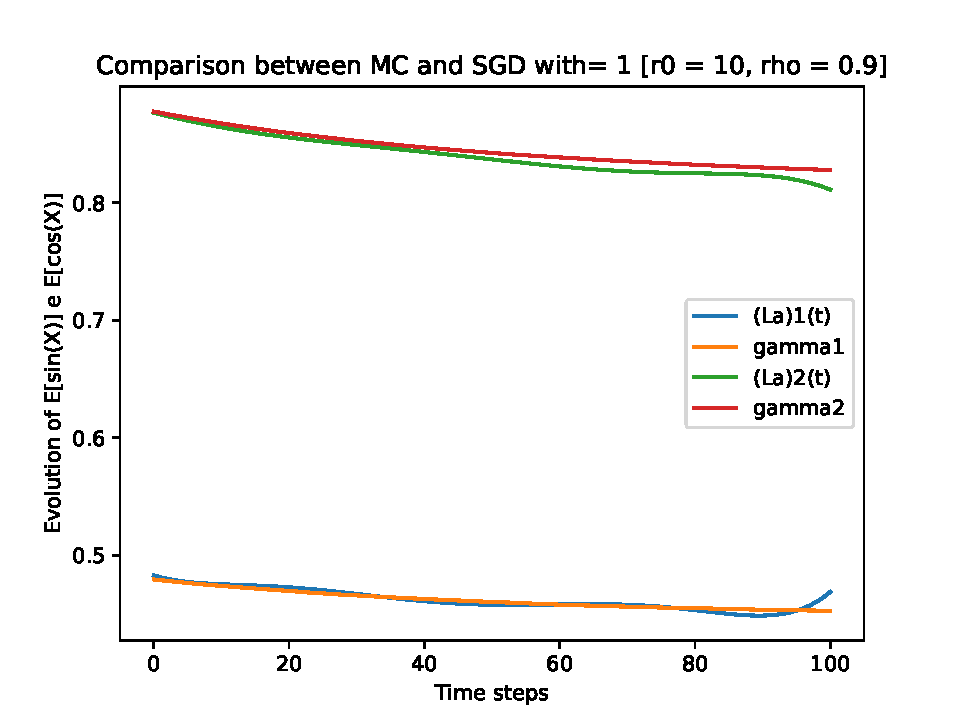
\includegraphics[width=0.9\textwidth]{images/graphs T = 1/n = 6, M = 1 sine and cosine.pdf}
\end{figure}
\begin{figure}[H]
\centering
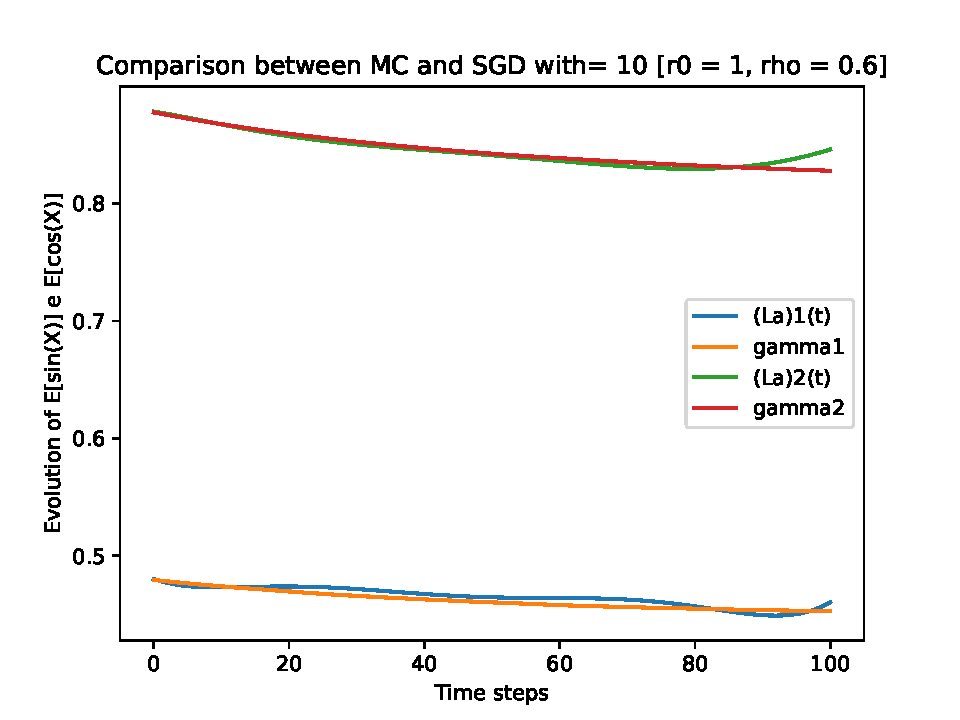
\includegraphics[width=0.9\textwidth]{images/graphs T = 1/n = 6, M = 10 sine and cosine.pdf}
\end{figure}
\begin{figure}[H]
\centering
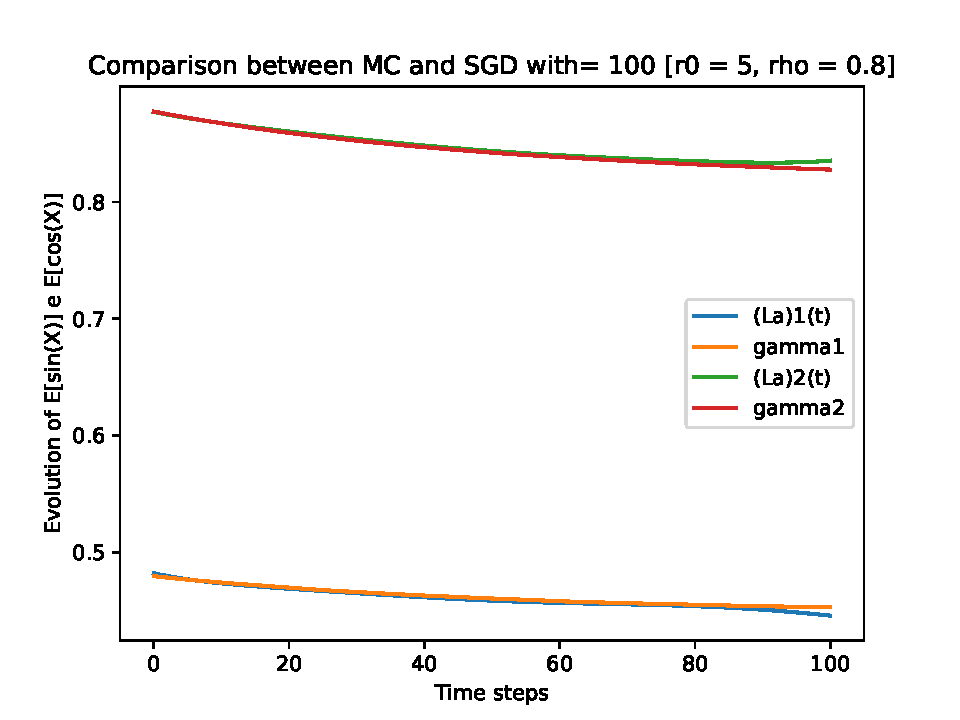
\includegraphics[width=0.9\textwidth]{images/graphs T = 1/n = 6, M = 100 sine and cosine.pdf}
\end{figure}
\begin{figure}[H]
\centering
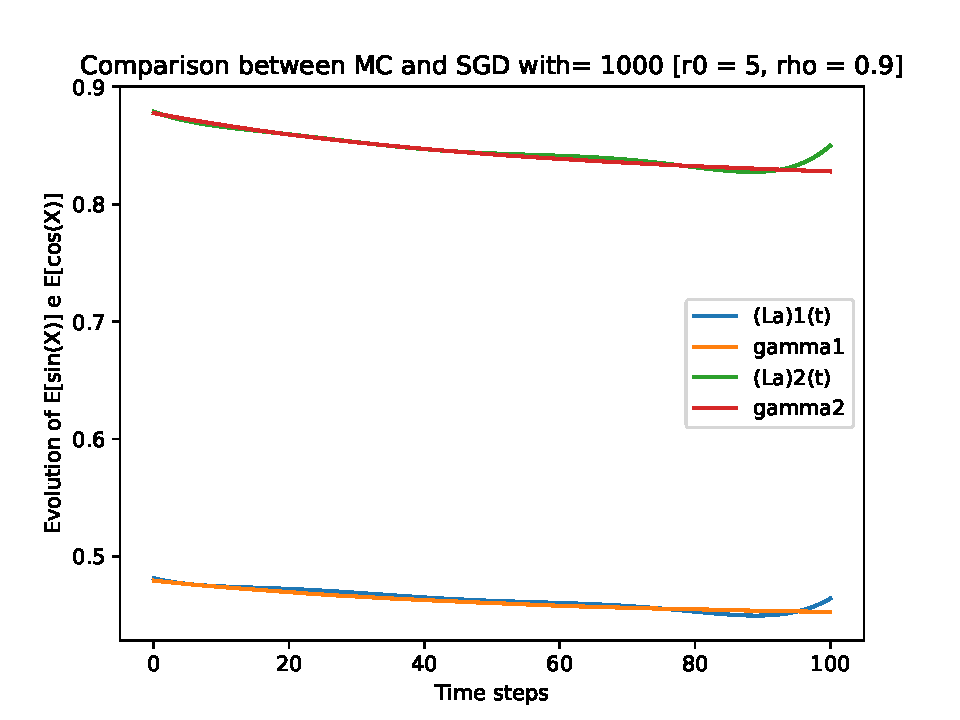
\includegraphics[width=0.9\textwidth]{images/graphs T = 1/n = 6, M = 1000 sine and cosine.pdf}
\end{figure}
\begin{figure}[H]
\centering
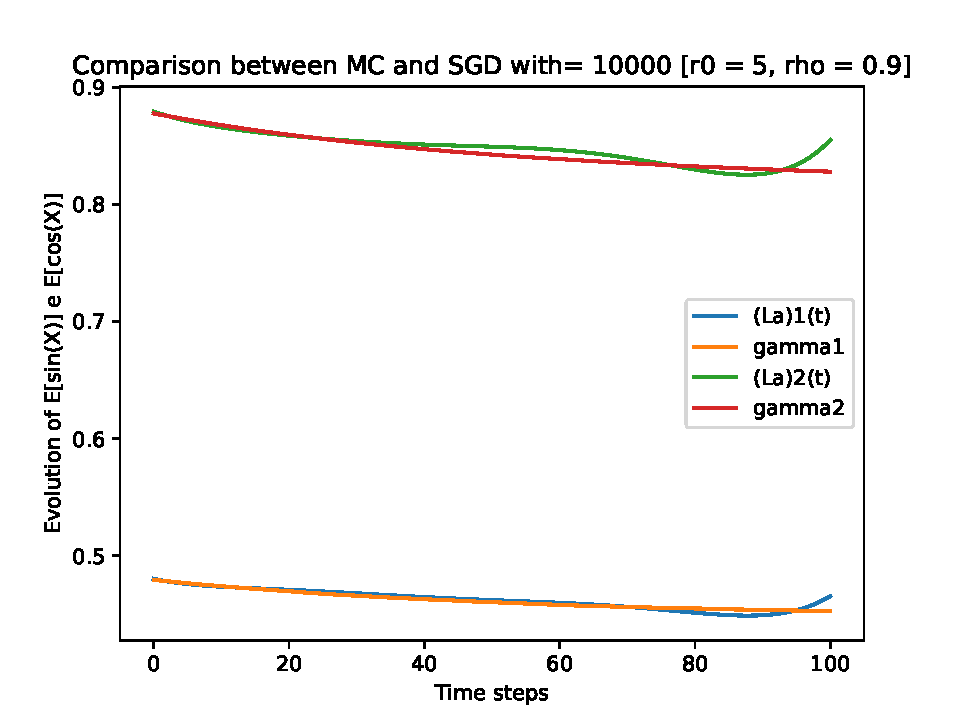
\includegraphics[width=0.9\textwidth]{images/graphs T = 1/n = 6, M = 10000 sine and cosine.pdf}
\end{figure}
\newpage
\section{T = 2}
\section*{Case n = 3} 
\begin{table}[H]
\centering
\addtolength{\leftskip}{-1.5cm}
\addtolength{\rightskip}{-1.5cm}
\begin{tabular}{|c|ll|}
\hline
$ $ & $r_0 = 1$ & $r_0 = 5$ \\
\hline
$\rho = 0.6$ & 22.35 & 80.57 \\

$\rho = 0.7$ & 12.28 & 42.48 \\

$\rho = 0.8$ & 34.07 & 19.80 \\

$\rho = 0.9$ & 94.34 & 23.10 \\
\hline
\end{tabular}
\caption{Average execution
 times (in seconds $s$) with $M = 1$}
\end{table}
\begin{table}[H]
\centering
\addtolength{\leftskip}{-1.5cm}
\addtolength{\rightskip}{-1.5cm}
\begin{tabular}{|c|lllllllll|}
\hline
$ $ & $r_0 = 1$ & $r_0 = 1$ & $r_0 = 1$ & $r_0 = 5$ & $r_0 = 5$ & $r_0 = 5$ & $r_0 = 10$ & $r_0 = 10$ & $r_0 = 10$  \\
$ $ & min & max & average & min & max & average & min & max & average \\ 
\hline
$\rho = 0.6$ & 1070 & 3030 & 1798 & 3760 & 10900 & 6485 &  & overflow &  \\

$\rho = 0.7$ & 200 & 1460 & 992 & 1310 & 4700 & 3419 &  & overflow &  \\

$\rho = 0.8$ & 360 & 8220 & 2753 & 950 & 2600 & 1597 &  & overflow & \\

$\rho = 0.9$ & 560 & 24050 & 7602 & 880 & 2870 & 1863 &  & overflow & \\
\hline
\end{tabular}
\caption{Number of iterations $m$ to achieve convergence with $M = 1$}
\end{table}
\begin{table}[H]
\centering
\addtolength{\leftskip}{-1.5cm}
\addtolength{\rightskip}{-1.5cm}
\begin{tabular}{|c|ll|}
\hline
$ $ & $r_0 = 1$ & $r_0 = 5$ \\
\hline
$\rho = 0.6$ & 3.91 & 11.72 \\

$\rho = 0.7$ & 1.98 & 7.75 \\

$\rho = 0.8$ & 7.45 & 5.10 \\

$\rho = 0.9$ & 5.94 & 4.78 \\
\hline
\end{tabular}
\caption{Average execution
 times (in seconds $s$) with $M = 10$}
\end{table}
\begin{table}[H]
\centering
\addtolength{\leftskip}{-1.5cm}
\addtolength{\rightskip}{-1.5cm}
\begin{tabular}{|c|lllllllll|}
\hline
$ $ & $r_0 = 1$ & $r_0 = 1$ & $r_0 = 1$ & $r_0 = 5$ & $r_0 = 5$ & $r_0 = 5$ & $r_0 = 10$ & $r_0 = 10$ & $r_0 = 10$  \\
$ $ & min & max & average & min & max & average & min & max & average \\ 
\hline
$\rho = 0.6$ & 50 & 500 & 275 & 260 & 1360 & 819 &  & overflow &  \\

$\rho = 0.7$ & 20 & 440 & 139 & 190 & 1110 & 544 &  & overflow &  \\

$\rho = 0.8$ & 80 & 2130 & 492 & 140 & 640 & 357 &  & overflow & \\

$\rho = 0.9$ & 40 & 1300 & 416 & 120 & 830 & 335 &  & overflow & \\
\hline
\end{tabular}
\caption{Number of iterations $m$ to achieve convergence with $M = 10$}
\end{table}
\begin{table}[H]
\centering
\addtolength{\leftskip}{-1.5cm}
\addtolength{\rightskip}{-1.5cm}
\begin{tabular}{|c|ll|}
\hline
$ $ & $r_0 = 1$ & $r_0 = 5$ \\
\hline
$\rho = 0.6$ & 1.2 & 2.03 \\

$\rho = 0.7$ & 0.78 & 2.05 \\

$\rho = 0.8$ & 1.26 & 1.67  \\

$\rho = 0.9$ & 0.98 & 1.60 \\
\hline
\end{tabular}
\caption{Average execution
 times (in seconds $s$) with $M = 100$}
\end{table}
\begin{table}[H]
\centering
\addtolength{\leftskip}{-1.5cm}
\addtolength{\rightskip}{-1.5cm}
\begin{tabular}{|c|lllllllll|}
\hline
$ $ & $r_0 = 1$ & $r_0 = 1$ & $r_0 = 1$ & $r_0 = 5$ & $r_0 = 5$ & $r_0 = 5$ & $r_0 = 10$ & $r_0 = 10$ & $r_0 = 10$  \\
$ $ & min & max & average & min & max & average & min & max & average \\ 
\hline
$\rho = 0.6$ & 10 & 140 & 50 & 20 & 260 & 85 &  & overflow &  \\

$\rho = 0.7$ & 10 & 50 & 33 & 30 & 150 & 86 &  & overflow &  \\

$\rho = 0.8$ & 10 & 160 & 53 & 30 & 130 & 70 &  & overflow & \\

$\rho = 0.9$ & 10 & 90 & 41 & 40 & 110 & 67 &  & overflow & \\
\hline
\end{tabular}
\caption{Number of iterations $m$ to achieve convergence with $M = 100$}
\end{table}
\begin{table}[H]
\centering
\addtolength{\leftskip}{-1.5cm}
\addtolength{\rightskip}{-1.5cm}
\begin{tabular}{|c|ll|}
\hline
$ $ & $r_0 = 1$ & $r_0 = 5$ \\
\hline
$\rho = 0.6$ & 1.02 & 5.35  \\

$\rho = 0.7$ & 0.88 & 3.42  \\

$\rho = 0.8$ & 0.88 & 2.31  \\

$\rho = 0.9$ & 1.64 & 2.29  \\
\hline
\end{tabular}
\caption{Average execution
 times (in seconds $s$) with $M = 1000$}
\end{table}
\begin{table}[H]
\centering
\addtolength{\leftskip}{-1.5cm}
\addtolength{\rightskip}{-1.5cm}
\begin{tabular}{|c|lllllllll|}
\hline
$ $ & $r_0 = 1$ & $r_0 = 1$ & $r_0 = 1$ & $r_0 = 5$ & $r_0 = 5$ & $r_0 = 5$ & $r_0 = 10$ & $r_0 = 10$ & $r_0 = 10$  \\
$ $ & min & max & average & min & max & average & min & max & average \\ 
\hline
$\rho = 0.6$ & 2 & 11 & 5.3 & 21 & 36 & 27.5 &  & overflow &  \\

$\rho = 0.7$ & 3 & 14 & 4.6 & 12 & 29 & 17.7 &  & overflow &  \\

$\rho = 0.8$ & 3 & 12 & 4.6 & 10 & 18 & 11.9 &  & overflow & \\

$\rho = 0.9$ & 3 & 29 & 8.5 & 8 & 25 & 11.9 &  & overflow & \\
\hline
\end{tabular}
\caption{Number of iterations $m$ to achieve convergence with $M = 1000$}
\end{table}
\begin{table}[H]
\centering
\addtolength{\leftskip}{-1.5cm}
\addtolength{\rightskip}{-1.5cm}
\begin{tabular}{|c|ll|}
\hline
$ $ & $r_0 = 1$ & $r_0 = 5$  \\
\hline
$\rho = 0.6$ & 4.67 & 38.12  \\

$\rho = 0.7$ & 4.30 & 24.13  \\

$\rho = 0.8$ & 5.42 & 19.99  \\

$\rho = 0.9$ & 5.61 & 15.43  \\
\hline
\end{tabular}
\caption{Average execution
 times (in seconds $s$) with $M = 10000$}
\end{table}
\begin{table}[H]
\centering
\addtolength{\leftskip}{-1.5cm}
\addtolength{\rightskip}{-1.5cm}
\begin{tabular}{|c|lllllllll|}
\hline
$ $ & $r_0 = 1$ & $r_0 = 1$ & $r_0 = 1$ & $r_0 = 5$ & $r_0 = 5$ & $r_0 = 5$ & $r_0 = 10$ & $r_0 = 10$ & $r_0 = 10$  \\
$ $ & min & max & average & min & max & average & min & max & average \\ 
\hline
$\rho = 0.6$ & 2 & 3 & 2.5 & 15 & 26 & 20 &  & overflow &  \\

$\rho = 0.7$ & 2 & 3 & 2.3 & 12 & 17 & 12.7 &  & overflow &  \\

$\rho = 0.8$ & 2 & 4 & 2.9 & 9 & 14 & 10.6 &  & overflow & \\

$\rho = 0.9$ & 3 & 3 & 3 & 8 & 9 & 8.2 &  & overflow & \\
\hline
\end{tabular}
\caption{Number of iterations $m$ to achieve convergence with $M = 10000$}
\end{table}
\begin{figure}[H]
\centering
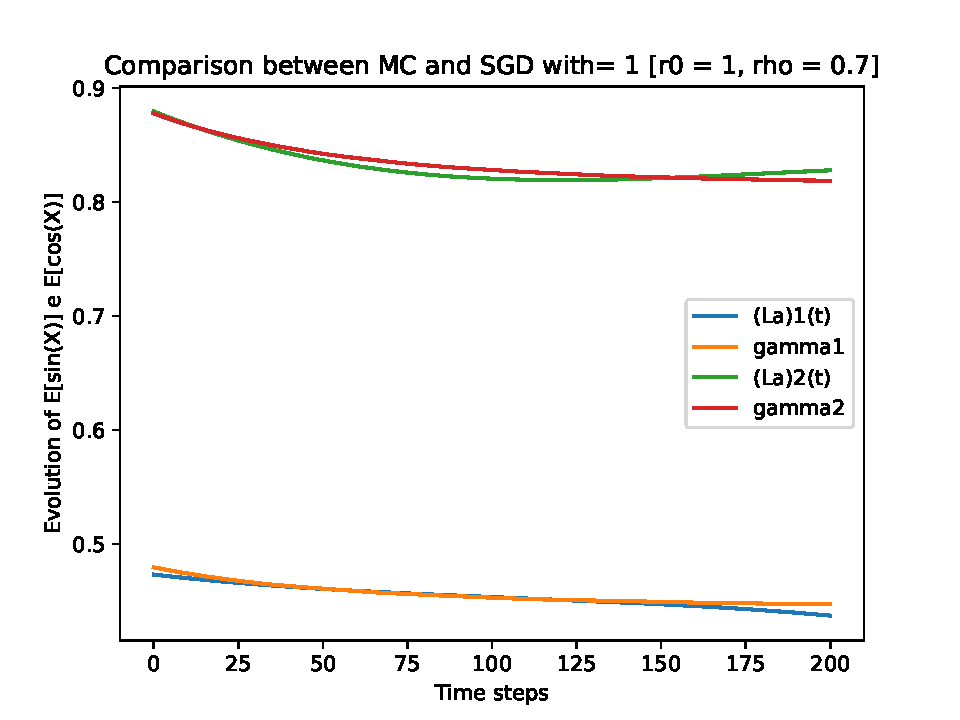
\includegraphics[width=0.9\textwidth]{images/graphs T = 2/n = 3, M = 1 sine and cosine.pdf}
\end{figure}
\begin{figure}[H]
\centering
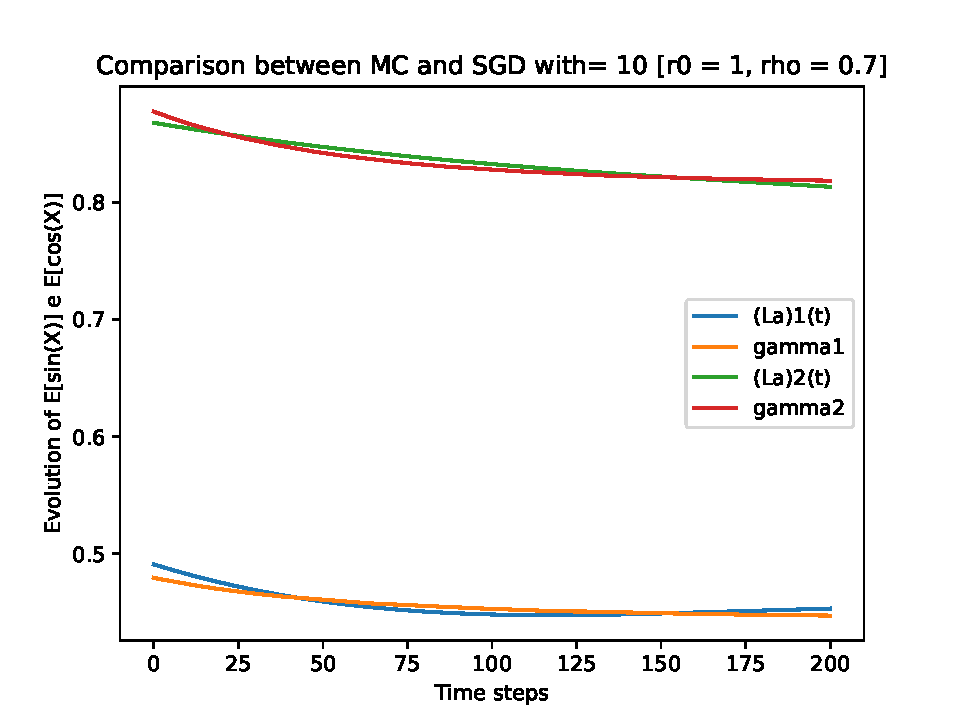
\includegraphics[width=0.9\textwidth]{images/graphs T = 2/n = 3, M = 10 sine and cosine.pdf}
\end{figure}
\begin{figure}[H]
\centering
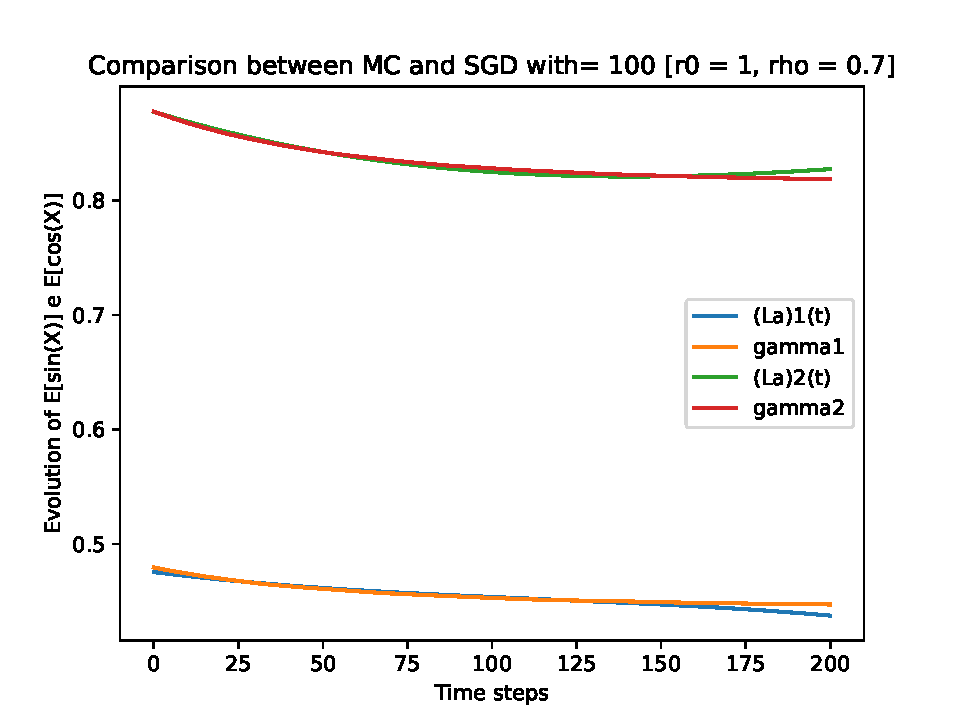
\includegraphics[width=0.9\textwidth]{images/graphs T = 2/n = 3, M = 100 sine and cosine.pdf}
\end{figure}
\begin{figure}[H]
\centering
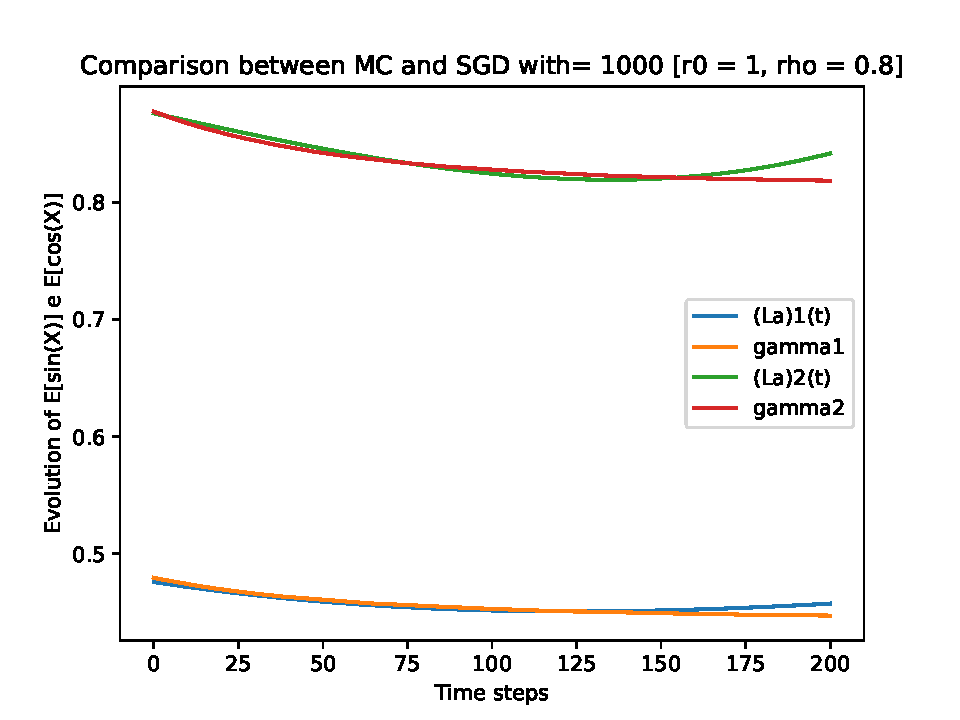
\includegraphics[width=0.9\textwidth]{images/graphs T = 2/n = 3, M = 1000 sine and cosine.pdf}
\end{figure}
\begin{figure}[H]
\centering
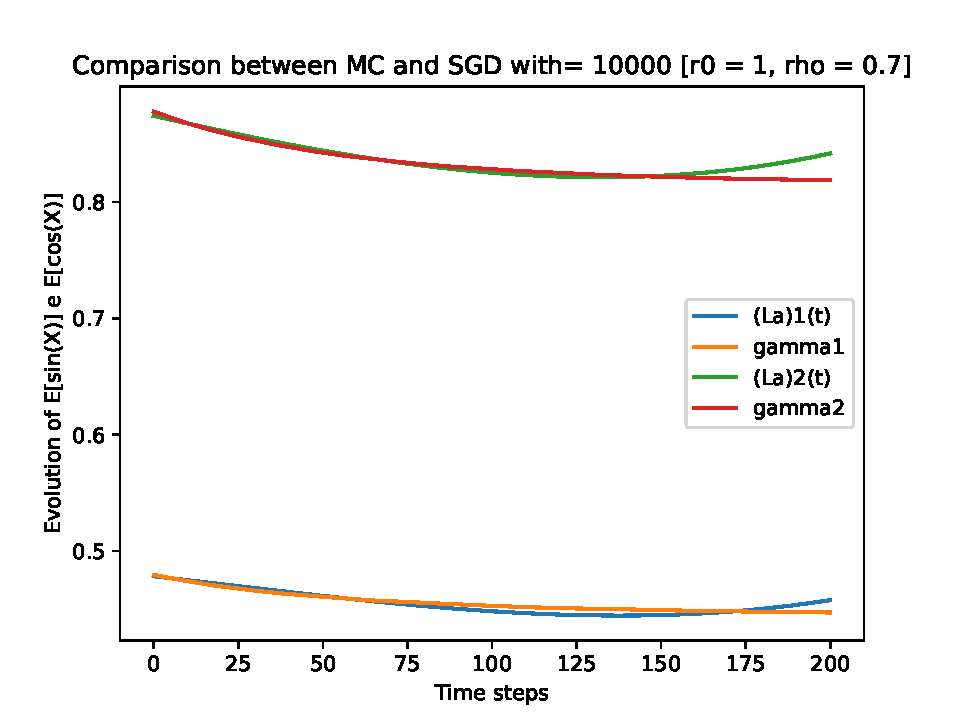
\includegraphics[width=0.9\textwidth]{images/graphs T = 2/n = 3, M = 10000 sine and cosine.pdf}
\end{figure}
\newpage
\section*{Case n = 4} 
\begin{table}[H]
\centering
\addtolength{\leftskip}{-1.5cm}
\addtolength{\rightskip}{-1.5cm}
\begin{tabular}{|c|ll|}
\hline
$ $ & $r_0 = 1$ & $r_0 = 5$ \\
\hline
$\rho = 0.6$ & 29.67 & 104.08 \\

$\rho = 0.7$ & 19.5 & 58.47 \\

$\rho = 0.8$ & 44.65 & 23.28 \\

$\rho = 0.9$ & 271.35 & 17.65 \\
\hline
\end{tabular}
\caption{Average execution
 times (in seconds $s$) with $M = 1$}
\end{table}
\begin{table}[H]
\centering
\addtolength{\leftskip}{-1.5cm}
\addtolength{\rightskip}{-1.5cm}
\begin{tabular}{|c|lllllllll|}
\hline
$ $ & $r_0 = 1$ & $r_0 = 1$ & $r_0 = 1$ & $r_0 = 5$ & $r_0 = 5$ & $r_0 = 5$ & $r_0 = 10$ & $r_0 = 10$ & $r_0 = 10$  \\
$ $ & min & max & average & min & max & average & min & max & average \\ 
\hline
$\rho = 0.6$ & 620 & 4050 & 2331 & 2890 & 11970 & 7908 &  & overflow &  \\

$\rho = 0.7$ & 670 & 3850 & 1529 & 1570 & 6540 & 4510 &  & overflow &  \\

$\rho = 0.8$ & 490 & 13550 & 3428 & 280 & 4230 & 1806 &  & overflow & \\

$\rho = 0.9$ & 1560 & 49999 & 20370.8 & 670 & 2480 & 1312 &  & overflow & \\
\hline
\end{tabular}
\caption{Number of iterations $m$ to achieve convergence with $M = 1$}
\end{table}
\begin{table}[H]
\centering
\addtolength{\leftskip}{-1.5cm}
\addtolength{\rightskip}{-1.5cm}
\begin{tabular}{|c|ll|}
\hline
$ $ & $r_0 = 1$ & $r_0 = 5$ \\
\hline
$\rho = 0.6$ & 4.56 & 13.23  \\

$\rho = 0.7$ & 4.85 & 7.61  \\

$\rho = 0.8$ & 6.83 & 5.09  \\

$\rho = 0.9$ & 29.93 & 4.01  \\
\hline
\end{tabular}
\caption{Average execution
 times (in seconds $s$) with $M = 10$}
\end{table}
\begin{table}[H]
\centering
\addtolength{\leftskip}{-1.5cm}
\addtolength{\rightskip}{-1.5cm}
\begin{tabular}{|c|lllllllll|}
\hline
$ $ & $r_0 = 1$ & $r_0 = 1$ & $r_0 = 1$ & $r_0 = 5$ & $r_0 = 5$ & $r_0 = 5$ & $r_0 = 10$ & $r_0 = 10$ & $r_0 = 10$  \\
$ $ & min & max & average & min & max & average & min & max & average \\ 
\hline
$\rho = 0.6$ & 80 & 620 & 310 & 340 & 1380 & 886 &  & overflow &  \\

$\rho = 0.7$ & 20 & 810 & 322 & 290 & 1090 & 519 &  & overflow &  \\

$\rho = 0.8$ & 40 & 2420 & 438 & 80 & 680 & 348 &  & overflow & \\

$\rho = 0.9$ & 60 & 6660 & 1909 & 110 & 690 & 273 &  & overflow & \\
\hline
\end{tabular}
\caption{Number of iterations $m$ to achieve convergence with $M = 10$}
\end{table}
\begin{table}[H]
\centering
\addtolength{\leftskip}{-1.5cm}
\addtolength{\rightskip}{-1.5cm}
\begin{tabular}{|c|ll|}
\hline
$ $ & $r_0 = 1$ & $r_0 = 5$ \\
\hline
$\rho = 0.6$ & 0.84 & 2.54  \\

$\rho = 0.7$ & 1.13 & 1.82  \\

$\rho = 0.8$ & 1.41 & 1.38  \\

$\rho = 0.9$ & 4.74 & 1.27  \\
\hline
\end{tabular}
\caption{Average execution
 times (in seconds $s$) with $M = 100$}
\end{table}
\begin{table}[H]
\centering
\addtolength{\leftskip}{-1.5cm}
\addtolength{\rightskip}{-1.5cm}
\begin{tabular}{|c|lllllllll|}
\hline
$ $ & $r_0 = 1$ & $r_0 = 1$ & $r_0 = 1$ & $r_0 = 5$ & $r_0 = 5$ & $r_0 = 5$ & $r_0 = 10$ & $r_0 = 10$ & $r_0 = 10$  \\
$ $ & min & max & average & min & max & average & min & max & average \\ 
\hline
$\rho = 0.6$ & 10 & 90 & 31 & 30 & 190 & 90 &  & overflow &  \\

$\rho = 0.7$ & 10 & 110 & 40 & 30 & 100 & 64 &  & overflow &  \\

$\rho = 0.8$ & 10 & 150 & 42 & 30 & 70 & 49 &  & overflow & \\

$\rho = 0.9$ & 20 & 950 & 169 & 10 & 80 & 45 &  & overflow & \\
\hline
\end{tabular}
\caption{Number of iterations $m$ to achieve convergence with $M = 100$}
\end{table}
\begin{table}[H]
\centering
\addtolength{\leftskip}{-1.5cm}
\addtolength{\rightskip}{-1.5cm}
\begin{tabular}{|c|ll|}
\hline
$ $ & $r_0 = 1$ & $r_0 = 5$ \\
\hline
$\rho = 0.6$ & 1.43 & 3.93 \\

$\rho = 0.7$ & 1.27 & 3.09 \\

$\rho = 0.8$ & 1.34 & 2.35 \\

$\rho = 0.9$ & 1.92 & 2.17 \\
\hline
\end{tabular}
\caption{Average execution
 times (in seconds $s$) with $M = 1000$}
\end{table}
\begin{table}[H]
\centering
\addtolength{\leftskip}{-1.5cm}
\addtolength{\rightskip}{-1.5cm}
\begin{tabular}{|c|lllllllll|}
\hline
$ $ & $r_0 = 1$ & $r_0 = 1$ & $r_0 = 1$ & $r_0 = 5$ & $r_0 = 5$ & $r_0 = 5$ & $r_0 = 10$ & $r_0 = 10$ & $r_0 = 10$  \\
$ $ & min & max & average & min & max & average & min & max & average \\ 
\hline
$\rho = 0.6$ & 4 & 11 & 6 & 13 & 20 & 16.4 &  & overflow &  \\

$\rho = 0.7$ & 3 & 11 & 5.3 & 10 & 21 & 12.8 &  & overflow &  \\

$\rho = 0.8$ & 4 & 11 & 5.6 & 8 & 13 & 9.7 &  & overflow & \\

$\rho = 0.9$ & 4 & 23 & 8 & 7 & 14 & 9.1 &  &overflow  & \\
\hline
\end{tabular}
\caption{Number of iterations $m$ to achieve convergence with $M = 1000$}
\end{table}
\begin{table}[H]
\centering
\addtolength{\leftskip}{-1.5cm}
\addtolength{\rightskip}{-1.5cm}
\begin{tabular}{|c|ll|}
\hline
$ $ & $r_0 = 1$ & $r_0 = 5$  \\
\hline
$\rho = 0.6$ & 7.24 & 30.59 \\

$\rho = 0.7$ & 7.20 & 22.75 \\

$\rho = 0.8$ & 7.77 & 18.19 \\

$\rho = 0.9$ & 8.51 & 16.25 \\
\hline
\end{tabular}
\caption{Average execution
 times (in seconds $s$) with $M = 10000$}
\end{table}
\begin{table}[H]
\centering
\addtolength{\leftskip}{-1.5cm}
\addtolength{\rightskip}{-1.5cm}
\begin{tabular}{|c|lllllllll|}
\hline
$ $ & $r_0 = 1$ & $r_0 = 1$ & $r_0 = 1$ & $r_0 = 5$ & $r_0 = 5$ & $r_0 = 5$ & $r_0 = 10$ & $r_0 = 10$ & $r_0 = 10$  \\
$ $ & min & max & average & min & max & average & min & max & average \\ 
\hline
$\rho = 0.6$ & 3 & 4 & 3.1 & 13 & 13 & 13 &  & overflow &  \\

$\rho = 0.7$ & 3 & 4 & 3.1 & 10 & 10 & 10 &  & overflow &  \\

$\rho = 0.8$ & 3 & 4 & 3.3 & 8 & 8 & 8 &  & overflow & \\

$\rho = 0.9$ & 3 & 4 & 3.6 & 7 & 7 & 7 &  & overflow & \\
\hline
\end{tabular}
\caption{Number of iterations $m$ to achieve convergence with $M = 10000$}
\end{table}
\begin{figure}[H]
\centering
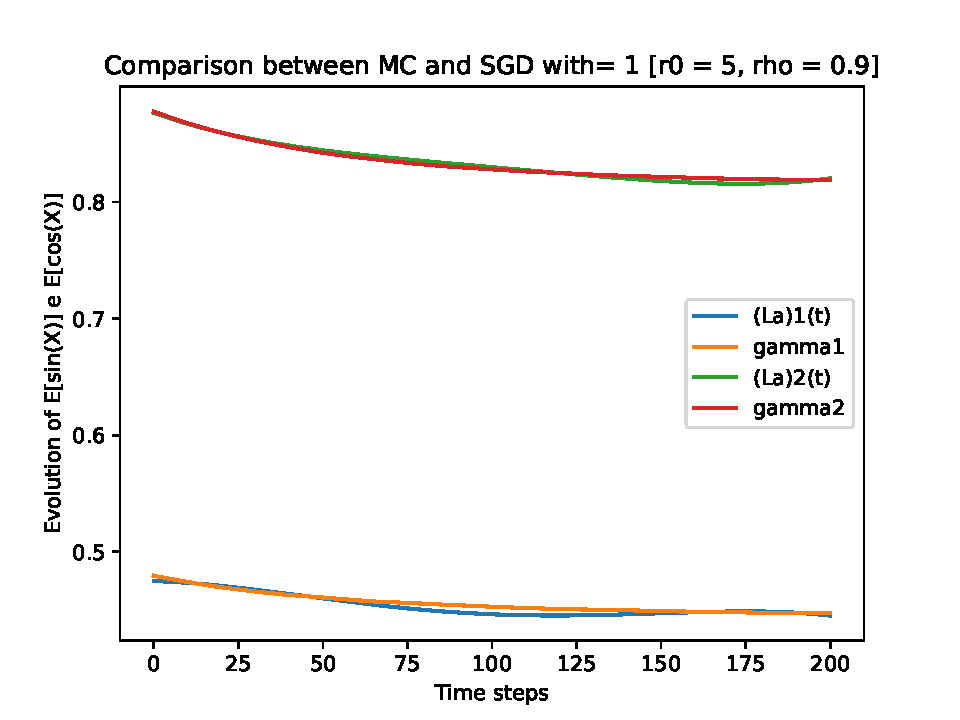
\includegraphics[width=0.9\textwidth]{images/graphs T = 2/n = 4, M = 1 sine and cosine.pdf}
\end{figure}
\begin{figure}[H]
\centering
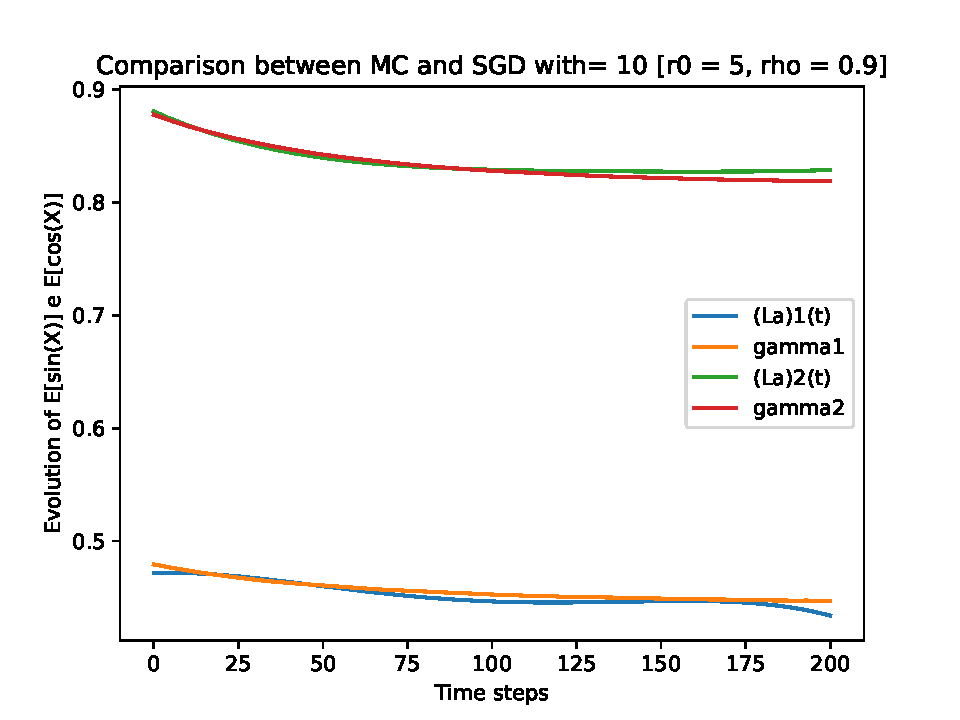
\includegraphics[width=0.9\textwidth]{images/graphs T = 2/n = 4, M = 10 sine and cosine.pdf}
\end{figure}
\begin{figure}[H]
\centering
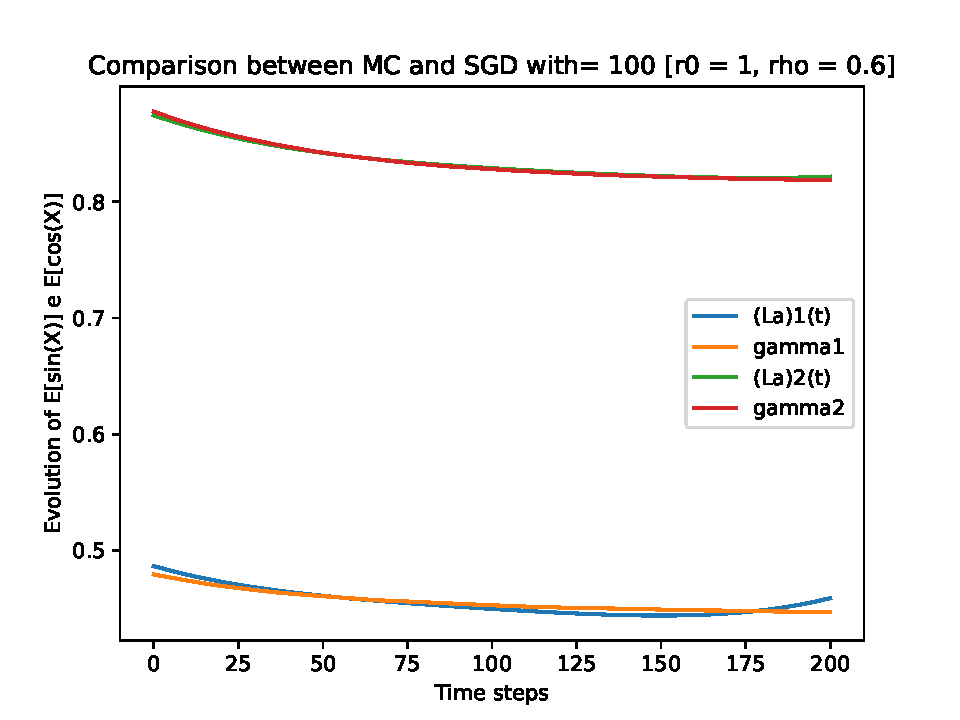
\includegraphics[width=0.9\textwidth]{images/graphs T = 2/n = 4, M = 100 sine and cosine.pdf}
\end{figure}
\begin{figure}[H]
\centering
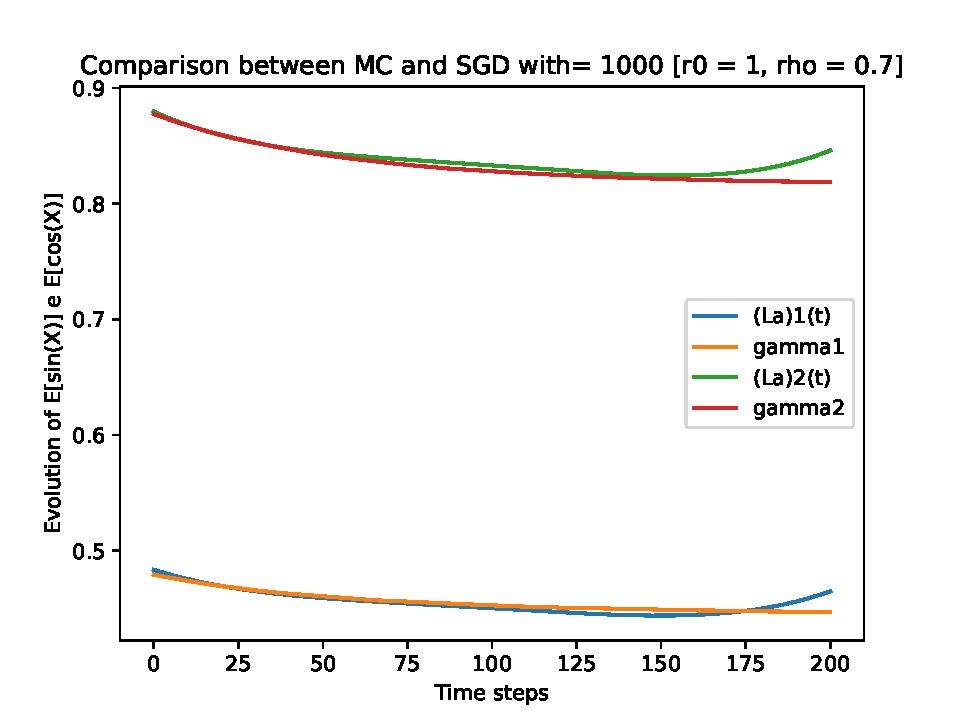
\includegraphics[width=0.9\textwidth]{images/graphs T = 2/n = 4, M = 1000 sine and cosine.pdf}
\end{figure}
\begin{figure}[H]
\centering
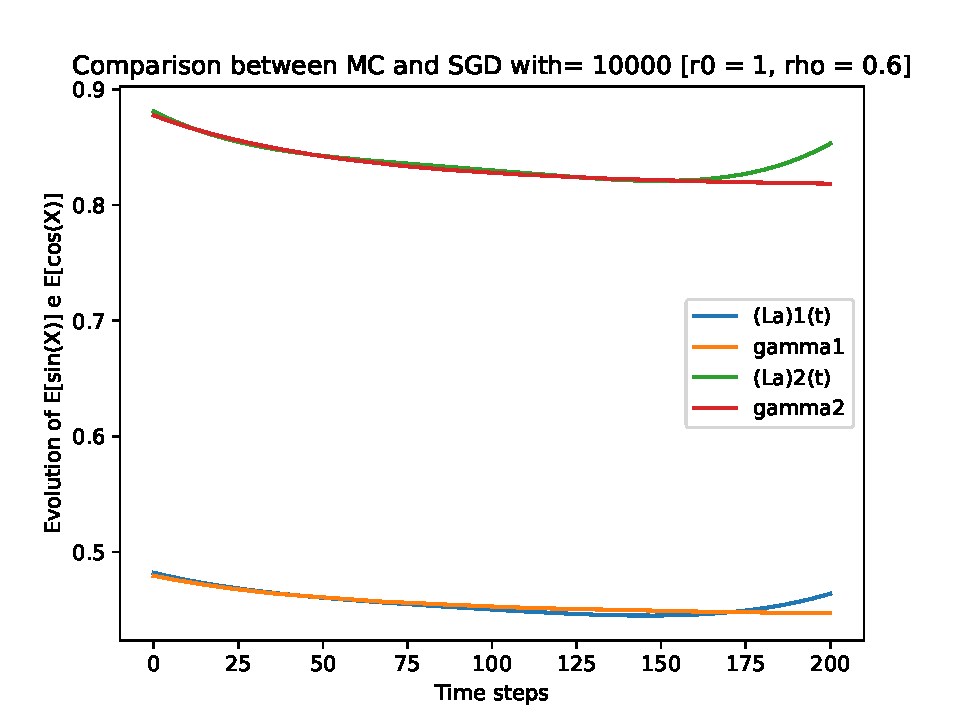
\includegraphics[width=0.9\textwidth]{images/graphs T = 2/n = 4, M = 10000 sine and cosine.pdf}
\end{figure}
\newpage
\section*{Case n = 5} 
\begin{table}[H]
\centering
\addtolength{\leftskip}{-1.5cm}
\addtolength{\rightskip}{-1.5cm}
\begin{tabular}{|c|ll|}
\hline
$ $ & $r_0 = 1$ & $r_0 = 5$ \\
\hline
$\rho = 0.6$ & 28.57 & 133.75 \\

$\rho = 0.7$ & 33.20 & 54.61 \\

$\rho = 0.8$ & 59.02 & 42.73 \\

$\rho = 0.9$ &  306.42 & 20.43 \\
\hline
\end{tabular}
\caption{Average execution
 times (in seconds $s$) with $M = 1$}
\end{table}
\begin{table}[H]
\centering
\addtolength{\leftskip}{-1.5cm}
\addtolength{\rightskip}{-1.5cm}
\begin{tabular}{|c|lllllllll|}
\hline
$ $ & $r_0 = 1$ & $r_0 = 1$ & $r_0 = 1$ & $r_0 = 5$ & $r_0 = 5$ & $r_0 = 5$ & $r_0 = 10$ & $r_0 = 10$ & $r_0 = 10$  \\
$ $ & min & max & average & min & max & average & min & max & average \\ 
\hline
$\rho = 0.6$ & 820 & 3420 & 2167 & 4540 & 17080 & 10248 &  & overflow &  \\

$\rho = 0.7$ & 490 & 6630 & 2459 & 2280 & 8430 & 4194 &  & overflow &  \\

$\rho = 0.8$ & 470 & 9120 & 4432 & 1410 & 7030 & 3278 &  & overflow & \\

$\rho = 0.9$ & 1160 & 49999 & 23456.7 & 400 & 4680 & 1570 &  & overflow & \\
\hline
\end{tabular}
\caption{Number of iterations $m$ to achieve convergence with $M = 1$}
\end{table}
\begin{table}[H]
\centering
\addtolength{\leftskip}{-1.5cm}
\addtolength{\rightskip}{-1.5cm}
\begin{tabular}{|c|ll|}
\hline
$ $ & $r_0 = 1$ & $r_0 = 5$ \\
\hline
$\rho = 0.6$ & 4.13 & 13.39 \\

$\rho = 0.7$ & 5.30 & 7.85  \\

$\rho = 0.8$ & 18.94 & 3.82 \\

$\rho = 0.9$ & 53.15 & 5.07 \\
\hline
\end{tabular}
\caption{Average execution
 times (in seconds $s$) with $M = 10$}
\end{table}
\begin{table}[H]
\centering
\addtolength{\leftskip}{-1.5cm}
\addtolength{\rightskip}{-1.5cm}
\begin{tabular}{|c|lllllllll|}
\hline
$ $ & $r_0 = 1$ & $r_0 = 1$ & $r_0 = 1$ & $r_0 = 5$ & $r_0 = 5$ & $r_0 = 5$ & $r_0 = 10$ & $r_0 = 10$ & $r_0 = 10$  \\
$ $ & min & max & average & min & max & average & min & max & average \\ 
\hline
$\rho = 0.6$ & 90 & 490 & 272 & 380 & 1610 & 883 &  & overflow &  \\

$\rho = 0.7$ & 100 & 570 & 333 & 180 & 950 & 517 &  & overflow &  \\

$\rho = 0.8$ & 70 & 6300 & 1230 & 90 & 510 & 252 &  & overflow & \\

$\rho = 0.9$ & 80 & 24990 & 3503 & 150 & 1130 & 335 &  & overflow & \\
\hline
\end{tabular}
\caption{Number of iterations $m$ to achieve convergence with $M = 10$}
\end{table}
\begin{table}[H]
\centering
\addtolength{\leftskip}{-1.5cm}
\addtolength{\rightskip}{-1.5cm}
\begin{tabular}{|c|ll|}
\hline
$ $ & $r_0 = 1$ & $r_0 = 5$ \\
\hline
$\rho = 0.6$ & 1.99 & 2.05  \\

$\rho = 0.7$ & 1.05 & 2.14  \\

$\rho = 0.8$ & 1.84 & 2.11  \\

$\rho = 0.9$ & 3.72 & 1.92  \\
\hline
\end{tabular}
\caption{Average execution
 times (in seconds $s$) with $M = 100$}
\end{table}
\begin{table}[H]
\centering
\addtolength{\leftskip}{-1.5cm}
\addtolength{\rightskip}{-1.5cm}
\begin{tabular}{|c|lllllllll|}
\hline
$ $ & $r_0 = 1$ & $r_0 = 1$ & $r_0 = 1$ & $r_0 = 5$ & $r_0 = 5$ & $r_0 = 5$ & $r_0 = 10$ & $r_0 = 10$ & $r_0 = 10$  \\
$ $ & min & max & average & min & max & average & min & max & average \\ 
\hline
$\rho = 0.6$ & 20 & 190 & 68 & 40 & 130 & 70 &  & overflow &  \\

$\rho = 0.7$ & 10 & 80 & 36 & 20 & 170 & 73 &  & overflow &  \\

$\rho = 0.8$ & 10 & 180 & 63 & 30 & 150 & 72 &  & overflow & \\

$\rho = 0.9$ & 10 & 680 & 127 & 30 & 120 & 65 &  & overflow & \\
\hline
\end{tabular}
\caption{Number of iterations $m$ to achieve convergence with $M = 100$}
\end{table}
\begin{table}[H]
\centering
\addtolength{\leftskip}{-1.5cm}
\addtolength{\rightskip}{-1.5cm}
\begin{tabular}{|c|ll|}
\hline
$ $ & $r_0 = 1$ & $r_0 = 5$  \\
\hline
$\rho = 0.6$ & 1.59 & 3.27  \\

$\rho = 0.7$ & 1.98 & 2.5  \\

$\rho = 0.8$ & 1.86 & 2.56  \\

$\rho = 0.9$ & 2.85 & 1.93  \\
\hline
\end{tabular}
\caption{Average execution
 times (in seconds $s$) with $M = 1000$}
\end{table}
\begin{table}[H]
\centering
\addtolength{\leftskip}{-1.5cm}
\addtolength{\rightskip}{-1.5cm}
\begin{tabular}{|c|lllllllll|}
\hline
$ $ & $r_0 = 1$ & $r_0 = 1$ & $r_0 = 1$ & $r_0 = 5$ & $r_0 = 5$ & $r_0 = 5$ & $r_0 = 10$ & $r_0 = 10$ & $r_0 = 10$  \\
$ $ & min & max & average & min & max & average & min & max & average \\ 
\hline
$\rho = 0.6$ & 4 & 10 & 6.1 & 10 & 17 & 12.4 &  & overflow &  \\

$\rho = 0.7$ & 4 & 16 & 7.6 & 8 & 13 & 9.6 &  & overflow &  \\

$\rho = 0.8$ & 5 & 12 & 7.1 & 7 & 14 & 9.8 &  & overflow & \\

$\rho = 0.9$ & 7 & 18 & 11 & 5 & 12 & 7.4 &  & overflow & \\
\hline
\end{tabular}
\caption{Number of iterations $m$ to achieve convergence with $M = 1000$}
\end{table}
\begin{table}[H]
\centering
\addtolength{\leftskip}{-1.5cm}
\addtolength{\rightskip}{-1.5cm}
\begin{tabular}{|c|ll|}
\hline
$ $ & $r_0 = 1$ & $r_0 = 5$  \\
\hline
$\rho = 0.6$ & 10.72 & 26.45 \\

$\rho = 0.7$ & 11.51 & 21.05 \\

$\rho = 0.8$ & 15.16 & 15.97  \\

$\rho = 0.9$ & 16.24 & 13.36  \\
\hline
\end{tabular}
\caption{Average execution
 times (in seconds $s$) with $M = 10000$}
\end{table}
\begin{table}[H]
\centering
\addtolength{\leftskip}{-1.5cm}
\addtolength{\rightskip}{-1.5cm}
\begin{tabular}{|c|lllllllll|}
\hline
$ $ & $r_0 = 1$ & $r_0 = 1$ & $r_0 = 1$ & $r_0 = 5$ & $r_0 = 5$ & $r_0 = 5$ & $r_0 = 10$ & $r_0 = 10$ & $r_0 = 10$  \\
$ $ & min & max & average & min & max & average & min & max & average \\ 
\hline
$\rho = 0.6$ & 4 & 5 & 4.1 & 10 & 11 & 10.1 &  & overflow &  \\

$\rho = 0.7$ & 4 & 5 & 4.4 & 8 & 8 & 8 &  & overflow &  \\

$\rho = 0.8$ & 5 & 8 & 5.8 & 6 & 7 & 6.1 &  & overflow & \\

$\rho = 0.9$ & 5 & 8 & 6.2 & 5 & 6 & 5.1 &  & overflow & \\
\hline
\end{tabular}
\caption{Number of iterations $m$ to achieve convergence with $M = 10000$}
\end{table}
\begin{figure}[H]
\centering
\includegraphics[width=0.9\textwidth]{images/graphs T = 2/n = 5, M = 1 sine and cosine.pdf}
\end{figure}
\begin{figure}[H]
\centering
\includegraphics[width=0.9\textwidth]{images/graphs T = 2/n = 5, M = 10 sine and cosine.pdf}
\end{figure}
\begin{figure}[H]
\centering
\includegraphics[width=0.9\textwidth]{images/graphs T = 2/n = 5, M = 100 sine and cosine.pdf}
\end{figure}
\begin{figure}[H]
\centering
\includegraphics[width=0.9\textwidth]{images/graphs T = 2/n = 5, M = 1000 sine and cosine.pdf}
\end{figure}
\begin{figure}[H]
\centering
\includegraphics[width=0.9\textwidth]{images/graphs T = 2/n = 5, M = 10000 sine and cosine.pdf}
\end{figure}
\newpage
\section*{Case n = 6} 
\begin{table}[H]
\centering
\addtolength{\leftskip}{-1.5cm}
\addtolength{\rightskip}{-1.5cm}
\begin{tabular}{|c|lll|}
\hline
$ $ & $r_0 = 1$ & $r_0 = 5$ & $r_0 = 10$ \\
\hline
$\rho = 0.6$ & 32.08 & 143.46 &  \\

$\rho = 0.7$ & 17.72 & 59.82 &  \\

$\rho = 0.8$ & 45.81 & 38.29 & 56.83 \\

$\rho = 0.9$ & 415.62 & 20.29 & 33.01 \\
\hline
\end{tabular}
\caption{Average execution
 times (in seconds $s$) with $M = 1$}
\end{table}
\begin{table}[H]
\centering
\addtolength{\leftskip}{-1.5cm}
\addtolength{\rightskip}{-1.5cm}
\begin{tabular}{|c|lllllllll|}
\hline
$ $ & $r_0 = 1$ & $r_0 = 1$ & $r_0 = 1$ & $r_0 = 5$ & $r_0 = 5$ & $r_0 = 5$ & $r_0 = 10$ & $r_0 = 10$ & $r_0 = 10$  \\
$ $ & min & max & average & min & max & average & min & max & average \\ 
\hline
$\rho = 0.6$ & 530 & 5630 & 2424 & 4710 & 21280 & 10855 &  & overflow &  \\

$\rho = 0.7$ & 380 & 3370 & 1336 & 990 & 8130 & 4511 &  & overflow &  \\

$\rho = 0.8$ & 900 & 12100 & 3456 & 1050 & 4840 & 2893 & 2490 & 6850 & 4171 \\

$\rho = 0.9$ & 7640 & 49999 & 31384.5 & 440 & 4390 & 1532 & 1620 & 4050 & 2405\\
\hline
\end{tabular}
\caption{Number of iterations $m$ to achieve convergence with $M = 1$}
\end{table}
\begin{table}[H]
\centering
\addtolength{\leftskip}{-1.5cm}
\addtolength{\rightskip}{-1.5cm}
\begin{tabular}{|c|lll|}
\hline
$ $ & $r_0 = 1$ & $r_0 = 5$ & $r_0 = 10$ \\
\hline
$\rho = 0.6$ & 3.39 & 14.24 &  \\

$\rho = 0.7$ & 5.58 & 6.85 &  \\

$\rho = 0.8$ & 19.75 & 7.34 & 8.91 \\

$\rho = 0.9$ & 15.37 & 5.23 & 5.81 \\
\hline
\end{tabular}
\caption{Average execution
 times (in seconds $s$) with $M = 10$}
\end{table}
\begin{table}[H]
\centering
\addtolength{\leftskip}{-1.5cm}
\addtolength{\rightskip}{-1.5cm}
\begin{tabular}{|c|lllllllll|}
\hline
$ $ & $r_0 = 1$ & $r_0 = 1$ & $r_0 = 1$ & $r_0 = 5$ & $r_0 = 5$ & $r_0 = 5$ & $r_0 = 10$ & $r_0 = 10$ & $r_0 = 10$  \\
$ $ & min & max & average & min & max & average & min & max & average \\ 
\hline
$\rho = 0.6$ & 50 & 640 & 219 & 410 & 1280 & 917 &  & overflow &  \\

$\rho = 0.7$ & 60 & 710 & 359 & 130 & 900 & 442 &  & overflow &  \\

$\rho = 0.8$ & 90 & 7070 & 1271 & 90 & 870 & 472 & 290 & 990 & 569 \\

$\rho = 0.9$ & 130 & 2720 & 988 & 70 & 670 & 337 & 100 & 750 & 369\\
\hline
\end{tabular}
\caption{Number of iterations $m$ to achieve convergence with $M = 10$}
\end{table}
\begin{table}[H]
\centering
\addtolength{\leftskip}{-1.5cm}
\addtolength{\rightskip}{-1.5cm}
\begin{tabular}{|c|lll|}
\hline
$ $ & $r_0 = 1$ & $r_0 = 5$ & $r_0 = 10$ \\
\hline
$\rho = 0.6$ & 1.07 & 3.43 &  \\

$\rho = 0.7$ & 0.80 & 2.40 &  \\

$\rho = 0.8$ & 3.97 & 2.23 & 4.02 \\

$\rho = 0.9$ & 9.14 & 1.61 & 2.75 \\
\hline
\end{tabular}
\caption{Average execution
 times (in seconds $s$) with $M = 100$}
\end{table}
\begin{table}[H]
\centering
\addtolength{\leftskip}{-1.5cm}
\addtolength{\rightskip}{-1.5cm}
\begin{tabular}{|c|lllllllll|}
\hline
$ $ & $r_0 = 1$ & $r_0 = 1$ & $r_0 = 1$ & $r_0 = 5$ & $r_0 = 5$ & $r_0 = 5$ & $r_0 = 10$ & $r_0 = 10$ & $r_0 = 10$  \\
$ $ & min & max & average & min & max & average & min & max & average \\ 
\hline
$\rho = 0.6$ & 10 & 50 & 35 & 60 & 170 & 111 &  & overflow &  \\

$\rho = 0.7$ & 10 & 60 & 26 & 40 & 160 & 78 &  & overflow &  \\

$\rho = 0.8$ & 10 & 520 & 129 & 30 & 190 & 72 & 70 & 260 & 127 \\

$\rho = 0.9$ & 20 & 1540 & 295 & 20 & 80 & 52 & 50 & 140 & 88\\
\hline
\end{tabular}
\caption{Number of iterations $m$ to achieve convergence with $M = 100$}
\end{table}
\begin{table}[H]
\centering
\addtolength{\leftskip}{-1.5cm}
\addtolength{\rightskip}{-1.5cm}
\begin{tabular}{|c|lll|}
\hline
$ $ & $r_0 = 1$ & $r_0 = 5$ & $r_0 = 10$ \\
\hline
$\rho = 0.6$ & 2.03 & 3.15 &  \\

$\rho = 0.7$ & 3.47 & 2.27 &  \\

$\rho = 0.8$ & 3.84 & 2.44 & 7.27 \\

$\rho = 0.9$ & 3.87 & 1.91 & 7.67 \\
\hline
\end{tabular}
\caption{Average execution
 times (in seconds $s$) with $M = 1000$}
\end{table}
\begin{table}[H]
\centering
\addtolength{\leftskip}{-1.5cm}
\addtolength{\rightskip}{-1.5cm}
\begin{tabular}{|c|lllllllll|}
\hline
$ $ & $r_0 = 1$ & $r_0 = 1$ & $r_0 = 1$ & $r_0 = 5$ & $r_0 = 5$ & $r_0 = 5$ & $r_0 = 10$ & $r_0 = 10$ & $r_0 = 10$  \\
$ $ & min & max & average & min & max & average & min & max & average \\ 
\hline
$\rho = 0.6$ & 5 & 10 & 6.8 & 8 & 24 & 10.7 &  & overflow &  \\

$\rho = 0.7$ & 6 & 32 & 11.8 & 6 & 12 & 7.7 &  & overflow &  \\

$\rho = 0.8$ & 7 & 29 & 13 & 5 & 15 & 8.3 & 20 & 31 & 23.4 \\

$\rho = 0.9$ & 8 & 32 & 13.1 & 5 & 10 & 6.5 & 13 & 50 & 24.7\\
\hline
\end{tabular}
\caption{Number of iterations $m$ to achieve convergence with $M = 1000$}
\end{table}
\begin{table}[H]
\centering
\addtolength{\leftskip}{-1.5cm}
\addtolength{\rightskip}{-1.5cm}
\begin{tabular}{|c|lll|}
\hline
$ $ & $r_0 = 1$ & $r_0 = 5$ & $r_0 = 10$ \\
\hline
$\rho = 0.6$ & 17.80 & 27.06 &  \\

$\rho = 0.7$ & 20.13 & 19.79 &  \\

$\rho = 0.8$ & 23.78 & 16.89 & 67.48 \\

$\rho = 0.9$ & 27.38 & 16.50 & 45.50 \\
\hline
\end{tabular}
\caption{Average execution
 times (in seconds $s$) with $M = 10000$}
\end{table}
\begin{table}[H]
\centering
\addtolength{\leftskip}{-1.5cm}
\addtolength{\rightskip}{-1.5cm}
\begin{tabular}{|c|lllllllll|}
\hline
$ $ & $r_0 = 1$ & $r_0 = 1$ & $r_0 = 1$ & $r_0 = 5$ & $r_0 = 5$ & $r_0 = 5$ & $r_0 = 10$ & $r_0 = 10$ & $r_0 = 10$  \\
$ $ & min & max & average & min & max & average & min & max & average \\ 
\hline
$\rho = 0.6$ & 5 & 7 & 5.4 & 8 & 9 & 8.2 &  & overflow &  \\

$\rho = 0.7$ & 6 & 7 & 6.1 & 6 & 6 & 6 &  & overflow &  \\

$\rho = 0.8$ & 7 & 8 & 7.2 & 5 & 6 & 5.1 & 17 & 24 & 18.8 \\

$\rho = 0.9$ & 7 & 9 & 8.3 & 5 & 5 & 5 & 12 & 17 & 13.6\\
\hline
\end{tabular}
\caption{Number of iterations $m$ to achieve convergence with $M = 10000$}
\end{table}
\begin{figure}[H]
\centering
\includegraphics[width=0.9\textwidth]{images/graphs T = 2/n = 6, M = 1 sine and cosine.pdf}
\end{figure}
\begin{figure}[H]
\centering
\includegraphics[width=0.9\textwidth]{images/graphs T = 2/n = 6, M = 10 sine and cosine.pdf}
\end{figure}
\begin{figure}[H]
\centering
\includegraphics[width=0.9\textwidth]{images/graphs T = 2/n = 6, M = 100 sine and cosine.pdf}
\end{figure}
\begin{figure}[H]
\centering
\includegraphics[width=0.9\textwidth]{images/graphs T = 2/n = 6, M = 1000 sine and cosine.pdf}
\end{figure}
\begin{figure}[H]
\centering
\includegraphics[width=0.9\textwidth]{images/graphs T = 2/n = 6, M = 10000 sine and cosine.pdf}
\end{figure}
\newpage
\section{T = 4}
\section*{Case n = 3} 
\begin{table}[H]
\centering
\addtolength{\leftskip}{-1.5cm}
\addtolength{\rightskip}{-1.5cm}
\begin{tabular}{|c|l|}
\hline
$ $ & $r_0 = 1$ \\
\hline
$\rho = 0.6$ & 148.41 \\

$\rho = 0.7$ & 98.14 \\

$\rho = 0.8$ & 99.71 \\

$\rho = 0.9$ & 269.29 \\
\hline
\end{tabular}
\caption{Average execution
 times (in seconds $s$) with $M = 1$}
\end{table}
\begin{table}[H]
\centering
\addtolength{\leftskip}{-1.5cm}
\addtolength{\rightskip}{-1.5cm}
\begin{tabular}{|c|lllllllll|}
\hline
$ $ & $r_0 = 1$ & $r_0 = 1$ & $r_0 = 1$ & $r_0 = 5$ & $r_0 = 5$ & $r_0 = 5$ & $r_0 = 10$ & $r_0 = 10$ & $r_0 = 10$  \\
$ $ & min & max & average & min & max & average & min & max & average \\ 
\hline
$\rho = 0.6$ & 3450 & 12910 & 6042 &  & overflow &  &  & overflow &  \\

$\rho = 0.7$ & 1150 & 7610 & 3999 &  & overflow &  &  & overflow &  \\

$\rho = 0.8$ & 1030 & 9770 & 4062 &  & overflow &  &  & overflow & \\

$\rho = 0.9$ & 900 & 49999 & 10512.9 &  & overflow &  &  & overflow & \\
\hline
\end{tabular}
\caption{Number of iterations $m$ to achieve convergence with $M = 1$}
\end{table}
\begin{table}[H]
\centering
\addtolength{\leftskip}{-1.5cm}
\addtolength{\rightskip}{-1.5cm}
\begin{tabular}{|c|l|}
\hline
$ $ & $r_0 = 1$  \\
\hline
$\rho = 0.6$ & 15.35  \\

$\rho = 0.7$ & 10.90 \\

$\rho = 0.8$ & 8.20 \\

$\rho = 0.9$ & 72.03 \\
\hline
\end{tabular}
\caption{Average execution
 times (in seconds $s$) with $M = 10$}
\end{table}
\begin{table}[H]
\centering
\addtolength{\leftskip}{-1.5cm}
\addtolength{\rightskip}{-1.5cm}
\begin{tabular}{|c|lllllllll|}
\hline
$ $ & $r_0 = 1$ & $r_0 = 1$ & $r_0 = 1$ & $r_0 = 5$ & $r_0 = 5$ & $r_0 = 5$ & $r_0 = 10$ & $r_0 = 10$ & $r_0 = 10$  \\
$ $ & min & max & average & min & max & average & min & max & average \\ 
\hline
$\rho = 0.6$ & 170 & 1180 & 521 &  & overflow &  &  & overflow &  \\

$\rho = 0.7$ & 110 & 740 & 370 &  & overflow &  &  & overflow &  \\

$\rho = 0.8$ & 110 & 690 & 280 &  & overflow &  &  & overflow & \\

$\rho = 0.9$ & 50 & 12920 & 2475 &  & overflow &  &  & overflow & \\
\hline
\end{tabular}
\caption{Number of iterations $m$ to achieve convergence with $M = 10$}
\end{table}
\begin{table}[H]
\centering
\addtolength{\leftskip}{-1.5cm}
\addtolength{\rightskip}{-1.5cm}
\begin{tabular}{|c|l|}
\hline
$ $ & $r_0 = 1$  \\
\hline
$\rho = 0.6$ & 3.48 \\

$\rho = 0.7$ & 5.24 \\

$\rho = 0.8$ & 5.58  \\

$\rho = 0.9$ & 15.62 \\
\hline
\end{tabular}
\caption{Average execution
 times (in seconds $s$) with $M = 100$}
\end{table}
\begin{table}[H]
\centering
\addtolength{\leftskip}{-1.5cm}
\addtolength{\rightskip}{-1.5cm}
\begin{tabular}{|c|lllllllll|}
\hline
$ $ & $r_0 = 1$ & $r_0 = 1$ & $r_0 = 1$ & $r_0 = 5$ & $r_0 = 5$ & $r_0 = 5$ & $r_0 = 10$ & $r_0 = 10$ & $r_0 = 10$  \\
$ $ & min & max & average & min & max & average & min & max & average \\ 
\hline
$\rho = 0.6$ & 30 & 140 & 68 &  & overflow &  &  & overflow &  \\

$\rho = 0.7$ & 20 & 310 & 101 &  & overflow &  &  & overflow &  \\

$\rho = 0.8$ & 30 & 330 & 108 &  & overflow &  &  & overflow & \\

$\rho = 0.9$ & 20 & 1360 & 307 &  & overflow &  &  & overflow & \\
\hline
\end{tabular}
\caption{Number of iterations $m$ to achieve convergence with $M = 100$}
\end{table}
\begin{table}[H]
\centering
\addtolength{\leftskip}{-1.5cm}
\addtolength{\rightskip}{-1.5cm}
\begin{tabular}{|c|l|}
\hline
$ $ & $r_0 = 1$  \\
\hline
$\rho = 0.6$ & 2.06  \\

$\rho = 0.7$ & 3.32  \\

$\rho = 0.8$ & 3.08  \\

$\rho = 0.9$ & 2.61  \\
\hline
\end{tabular}
\caption{Average execution
 times (in seconds $s$) with $M = 1000$}
\end{table}
\begin{table}[H]
\centering
\addtolength{\leftskip}{-1.5cm}
\addtolength{\rightskip}{-1.5cm}
\begin{tabular}{|c|lllllllll|}
\hline
$ $ & $r_0 = 1$ & $r_0 = 1$ & $r_0 = 1$ & $r_0 = 5$ & $r_0 = 5$ & $r_0 = 5$ & $r_0 = 10$ & $r_0 = 10$ & $r_0 = 10$  \\
$ $ & min & max & average & min & max & average & min & max & average \\ 
\hline
$\rho = 0.6$ & 4 & 8 & 4.7 &  & overflow &  &  & overflow &  \\

$\rho = 0.7$ & 4 & 16 & 7.8 &  & overflow &  &  & overflow &  \\

$\rho = 0.8$ & 3 & 19 & 7.1 &  & overflow &  &  & overflow & \\

$\rho = 0.9$ & 4 & 9 & 6 &  & overflow &  &  & overflow & \\
\hline
\end{tabular}
\caption{Number of iterations $m$ to achieve convergence with $M = 1000$}
\end{table}
\begin{table}[H]
\centering
\addtolength{\leftskip}{-1.5cm}
\addtolength{\rightskip}{-1.5cm}
\begin{tabular}{|c|l|}
\hline
$ $ & $r_0 = 1$   \\
\hline
$\rho = 0.6$ & 16.91  \\

$\rho = 0.7$ & 16.04  \\

$\rho = 0.8$ & 12.17  \\

$\rho = 0.9$ & 12.15  \\
\hline
\end{tabular}
\caption{Average execution
 times (in seconds $s$) with $M = 10000$}
\end{table}
\begin{table}[H]
\centering
\addtolength{\leftskip}{-1.5cm}
\addtolength{\rightskip}{-1.5cm}
\begin{tabular}{|c|lllllllll|}
\hline
$ $ & $r_0 = 1$ & $r_0 = 1$ & $r_0 = 1$ & $r_0 = 5$ & $r_0 = 5$ & $r_0 = 5$ & $r_0 = 10$ & $r_0 = 10$ & $r_0 = 10$  \\
$ $ & min & max & average & min & max & average & min & max & average \\ 
\hline
$\rho = 0.6$ & 4 & 4 & 4 &  & overflow &  &  & overflow &  \\

$\rho = 0.7$ & 4 & 4 & 4 &  & overflow &  &  & overflow &  \\

$\rho = 0.8$ & 3 & 3 & 3 &  & overflow &  &  & overflow & \\

$\rho = 0.9$ & 3 & 3 & 3 &  & overflow &  &  & overflow & \\
\hline
\end{tabular}
\caption{Number of iterations $m$ to achieve convergence with $M = 10000$}
\end{table}
\begin{figure}[H]
\centering
\includegraphics[width=0.9\textwidth]{images/graphs T = 4/n = 3, M = 1 sine and cosine.pdf}
\end{figure}
\begin{figure}[H]
\centering
\includegraphics[width=0.9\textwidth]{images/graphs T = 4/n = 3, M = 10 sine and cosine.pdf}
\end{figure}
\begin{figure}[H]
\centering
\includegraphics[width=0.9\textwidth]{images/graphs T = 4/n = 3, M = 100 sine and cosine.pdf}
\end{figure}
\begin{figure}[H]
\centering
\includegraphics[width=0.9\textwidth]{images/graphs T = 4/n = 3, M = 1000 sine and cosine.pdf}
\end{figure}
\begin{figure}[H]
\centering
\includegraphics[width=0.9\textwidth]{images/graphs T = 4/n = 3, M = 10000 sine and cosine.pdf}
\end{figure}
\newpage
\section*{Case n = 4} 
\begin{table}[H]
\centering
\addtolength{\leftskip}{-1.5cm}
\addtolength{\rightskip}{-1.5cm}
\begin{tabular}{|c|l|}
\hline
$ $ & $r_0 = 1$  \\
\hline
$\rho = 0.6$ & 145.11 \\

$\rho = 0.7$ & 102.23 \\

$\rho = 0.8$ & 177.10 \\

$\rho = 0.9$ & 890.75 \\
\hline
\end{tabular}
\caption{Average execution
 times (in seconds $s$) with $M = 1$}
\end{table}
\begin{table}[H]
\centering
\addtolength{\leftskip}{-1.5cm}
\addtolength{\rightskip}{-1.5cm}
\begin{tabular}{|c|lllllllll|}
\hline
$ $ & $r_0 = 1$ & $r_0 = 1$ & $r_0 = 1$ & $r_0 = 5$ & $r_0 = 5$ & $r_0 = 5$ & $r_0 = 10$ & $r_0 = 10$ & $r_0 = 10$  \\
$ $ & min & max & average & min & max & average & min & max & average \\ 
\hline
$\rho = 0.6$ & 3320 & 11980 & 5645 &  & overflow & &  & overflow &  \\

$\rho = 0.7$ & 1020 & 12700 & 3974 &  & overflow & &  & overflow &  \\

$\rho = 0.8$ & 740 & 25910 & 6650 &  & overflow & &  & overflow &  \\

$\rho = 0.9$ & 2470 & 49999 & 34868.5 &  & overflow & &  & overflow &  \\
\hline
\end{tabular}
\caption{Number of iterations $m$ to achieve convergence with $M = 1$}
\end{table}
\begin{table}[H]
\centering
\addtolength{\leftskip}{-1.5cm}
\addtolength{\rightskip}{-1.5cm}
\begin{tabular}{|c|l|}
\hline
$ $ & $r_0 = 1$  \\
\hline
$\rho = 0.6$ &  13.09 \\

$\rho = 0.7$ &  13.76 \\

$\rho = 0.8$ &  22.88 \\

$\rho = 0.9$ &  313.63 \\
\hline
\end{tabular}
\caption{Average execution
 times (in seconds $s$) with $M = 10$}
\end{table}
\begin{table}[H]
\centering
\addtolength{\leftskip}{-1.5cm}
\addtolength{\rightskip}{-1.5cm}
\begin{tabular}{|c|lllllllll|}
\hline
$ $ & $r_0 = 1$ & $r_0 = 1$ & $r_0 = 1$ & $r_0 = 5$ & $r_0 = 5$ & $r_0 = 5$ & $r_0 = 10$ & $r_0 = 10$ & $r_0 = 10$  \\
$ $ & min & max & average & min & max & average & min & max & average \\ 
\hline
$\rho = 0.6$ & 120 & 820 & 446 &  & overflow & &  & overflow &  \\

$\rho = 0.7$ & 250 & 820 & 473 &  & overflow & &  & overflow &  \\

$\rho = 0.8$ & 70 & 4380 & 778 &  & overflow & &  & overflow &  \\

$\rho = 0.9$ & 170 & 34500 & 10453 &  & overflow & &  & overflow &  \\
\hline
\end{tabular}
\caption{Number of iterations $m$ to achieve convergence with $M = 10$}
\end{table}
\begin{table}[H]
\centering
\addtolength{\leftskip}{-1.5cm}
\addtolength{\rightskip}{-1.5cm}
\begin{tabular}{|c|l|}
\hline
$ $ & $r_0 = 1$  \\
\hline
$\rho = 0.6$ & 4.71  \\

$\rho = 0.7$ & 2.61 \\

$\rho = 0.8$ & 5.88 \\

$\rho = 0.9$ & 37.38  \\
\hline
\end{tabular}
\caption{Average execution
 times (in seconds $s$) with $M = 100$}
\end{table}
\begin{table}[H]
\centering
\addtolength{\leftskip}{-1.5cm}
\addtolength{\rightskip}{-1.5cm}
\begin{tabular}{|c|lllllllll|}
\hline
$ $ & $r_0 = 1$ & $r_0 = 1$ & $r_0 = 1$ & $r_0 = 5$ & $r_0 = 5$ & $r_0 = 5$ & $r_0 = 10$ & $r_0 = 10$ & $r_0 = 10$  \\
$ $ & min & max & average & min & max & average & min & max & average \\ 
\hline
$\rho = 0.6$ & 40 & 160 & 88 &  & overflow & &  & overflow &  \\

$\rho = 0.7$ & 30 & 90 & 49 &  & overflow & &  & overflow &  \\

$\rho = 0.8$ & 10 & 390 & 108 &  & overflow & &  & overflow &  \\

$\rho = 0.9$ & 10 & 2810 & 703 &  & overflow & &  & overflow &  \\
\hline
\end{tabular}
\caption{Number of iterations $m$ to achieve convergence with $M = 100$}
\end{table}
\begin{table}[H]
\centering
\addtolength{\leftskip}{-1.5cm}
\addtolength{\rightskip}{-1.5cm}
\begin{tabular}{|c|l|}
\hline
$ $ & $r_0 = 1$  \\
\hline
$\rho = 0.6$ & 4.57 \\

$\rho = 0.7$ & 3.25 \\

$\rho = 0.8$ & 3.55 \\

$\rho = 0.9$ & 4.56 \\
\hline
\end{tabular}
\caption{Average execution
 times (in seconds $s$) with $M = 1000$}
\end{table}
\begin{table}[H]
\centering
\addtolength{\leftskip}{-1.5cm}
\addtolength{\rightskip}{-1.5cm}
\begin{tabular}{|c|lllllllll|}
\hline
$ $ & $r_0 = 1$ & $r_0 = 1$ & $r_0 = 1$ & $r_0 = 5$ & $r_0 = 5$ & $r_0 = 5$ & $r_0 = 10$ & $r_0 = 10$ & $r_0 = 10$  \\
$ $ & min & max & average & min & max & average & min & max & average \\ 
\hline
$\rho = 0.6$ & 4 & 18 & 9.5 &  & overflow & &  & overflow &  \\

$\rho = 0.7$ & 3 & 27 & 6.7 &  & overflow & &  & overflow &  \\

$\rho = 0.8$ & 3 & 18 & 7.4 &  & overflow & &  & overflow &  \\

$\rho = 0.9$ & 3 & 41 & 9.5 &  & overflow & &  & overflow &  \\
\hline
\end{tabular}
\caption{Number of iterations $m$ to achieve convergence with $M = 1000$}
\end{table}
\begin{table}[H]
\centering
\addtolength{\leftskip}{-1.5cm}
\addtolength{\rightskip}{-1.5cm}
\begin{tabular}{|c|l|}
\hline
$ $ & $r_0 = 1$  \\
\hline
$\rho = 0.6$ & 14.42 \\

$\rho = 0.7$ & 14.35 \\

$\rho = 0.8$ & 14.42 \\

$\rho = 0.9$ & 14.42 \\
\hline
\end{tabular}
\caption{Average execution
 times (in seconds $s$) with $M = 10000$}
\end{table}
\begin{table}[H]
\centering
\addtolength{\leftskip}{-1.5cm}
\addtolength{\rightskip}{-1.5cm}
\begin{tabular}{|c|lllllllll|}
\hline
$ $ & $r_0 = 1$ & $r_0 = 1$ & $r_0 = 1$ & $r_0 = 5$ & $r_0 = 5$ & $r_0 = 5$ & $r_0 = 10$ & $r_0 = 10$ & $r_0 = 10$  \\
$ $ & min & max & average & min & max & average & min & max & average \\ 
\hline
$\rho = 0.6$ & 3 & 3 & 3 &  & overflow & &  & overflow &  \\

$\rho = 0.7$ & 3 & 3 & 3 &  & overflow & &  & overflow &  \\

$\rho = 0.8$ & 3 & 3 & 3 &  & overflow & &  & overflow &  \\

$\rho = 0.9$ & 3 & 3 & 3 &  & overflow & &  & overflow &  \\
\hline
\end{tabular}
\caption{Number of iterations $m$ to achieve convergence with $M = 10000$}
\end{table}
\begin{figure}[H]
\centering
\includegraphics[width=0.9\textwidth]{images/graphs T = 4/n = 4, M = 1 sine and cosine.pdf}
\end{figure}
\begin{figure}[H]
\centering
\includegraphics[width=0.9\textwidth]{images/graphs T = 4/n = 4, M = 10 sine and cosine.pdf}
\end{figure}
\begin{figure}[H]
\centering
\includegraphics[width=0.9\textwidth]{images/graphs T = 4/n = 4, M = 100 sine and cosine.pdf}
\end{figure}
\begin{figure}[H]
\centering
\includegraphics[width=0.9\textwidth]{images/graphs T = 4/n = 4, M = 1000 sine and cosine.pdf}
\end{figure}
\begin{figure}[H]
\centering
\includegraphics[width=0.9\textwidth]{images/graphs T = 4/n = 4, M = 10000 sine and cosine.pdf}
\end{figure}
\newpage
\section*{Case n = 5} 
\begin{table}[H]
\centering
\addtolength{\leftskip}{-1.5cm}
\addtolength{\rightskip}{-1.5cm}
\begin{tabular}{|c|l|}
\hline
$ $ & $r_0 = 1$ \\
\hline
$\rho = 0.6$ & 187.19 \\

$\rho = 0.7$ & 100.55 \\

$\rho = 0.8$ & 343.00 \\

$\rho = 0.9$ & 1090.67 \\
\hline
\end{tabular}
\caption{Average execution
 times (in seconds $s$) with $M = 1$}
\end{table}
\begin{table}[H]
\centering
\addtolength{\leftskip}{-1.5cm}
\addtolength{\rightskip}{-1.5cm}
\begin{tabular}{|c|lllllllll|}
\hline
$ $ & $r_0 = 1$ & $r_0 = 1$ & $r_0 = 1$ & $r_0 = 5$ & $r_0 = 5$ & $r_0 = 5$ & $r_0 = 10$ & $r_0 = 10$ & $r_0 = 10$  \\
$ $ & min & max & average & min & max & average & min & max & average \\ 
\hline
$\rho = 0.6$ & 2410 & 17200 & 7261 &  & overflow &  &  & overflow &  \\

$\rho = 0.7$ & 1490 & 6980 & 3871 &  & overflow &  &  & overflow &  \\

$\rho = 0.8$ & 640 & 42740 & 13311 &  & overflow &  &  & overflow & \\

$\rho = 0.9$ & 2840 & 49999 & 41910.3 &  & overflow &  &  & overflow & \\
\hline
\end{tabular}
\caption{Number of iterations $m$ to achieve convergence with $M = 1$}
\end{table}
\begin{table}[H]
\centering
\addtolength{\leftskip}{-1.5cm}
\addtolength{\rightskip}{-1.5cm}
\begin{tabular}{|c|l|}
\hline
$ $ & $r_0 = 1$  \\
\hline
$\rho = 0.6$ & 30.49  \\

$\rho = 0.7$ & 13.62  \\

$\rho = 0.8$ & 22.37  \\

$\rho = 0.9$ & 423.87   \\
\hline
\end{tabular}
\caption{Average execution
 times (in seconds $s$) with $M = 10$}
\end{table}
\begin{table}[H]
\centering
\addtolength{\leftskip}{-1.5cm}
\addtolength{\rightskip}{-1.5cm}
\begin{tabular}{|c|lllllllll|}
\hline
$ $ & $r_0 = 1$ & $r_0 = 1$ & $r_0 = 1$ & $r_0 = 5$ & $r_0 = 5$ & $r_0 = 5$ & $r_0 = 10$ & $r_0 = 10$ & $r_0 = 10$  \\
$ $ & min & max & average & min & max & average & min & max & average \\ 
\hline
$\rho = 0.6$ & 120 & 3880 & 1020 &  & overflow &  &  & overflow &  \\

$\rho = 0.7$ & 180 & 860 & 455 &  & overflow &  &  & overflow &  \\

$\rho = 0.8$ & 120 & 2540 & 743 &  & overflow &  &  & overflow & \\

$\rho = 0.9$ & 190 & 38600 & 14211 &  & overflow &  &  & overflow & \\
\hline
\end{tabular}
\caption{Number of iterations $m$ to achieve convergence with $M = 10$}
\end{table}
\begin{table}[H]
\centering
\addtolength{\leftskip}{-1.5cm}
\addtolength{\rightskip}{-1.5cm}
\begin{tabular}{|c|l|}
\hline
$ $ & $r_0 = 1$  \\
\hline
$\rho = 0.6$ & 3.98  \\

$\rho = 0.7$ & 3.58  \\

$\rho = 0.8$ & 13.71  \\

$\rho = 0.9$ & 108.12   \\
\hline
\end{tabular}
\caption{Average execution
 times (in seconds $s$) with $M = 100$}
\end{table}
\begin{table}[H]
\centering
\addtolength{\leftskip}{-1.5cm}
\addtolength{\rightskip}{-1.5cm}
\begin{tabular}{|c|lllllllll|}
\hline
$ $ & $r_0 = 1$ & $r_0 = 1$ & $r_0 = 1$ & $r_0 = 5$ & $r_0 = 5$ & $r_0 = 5$ & $r_0 = 10$ & $r_0 = 10$ & $r_0 = 10$  \\
$ $ & min & max & average & min & max & average & min & max & average \\ 
\hline
$\rho = 0.6$ & 30 & 150 & 68 &  & overflow &  &  & overflow &  \\

$\rho = 0.7$ & 20 & 100 & 61 &  & overflow &  &  & overflow &  \\

$\rho = 0.8$ & 40 & 910 & 234 &  & overflow &  &  & overflow & \\

$\rho = 0.9$ & 10 & 12040 & 1843 &  & overflow &  &  & overflow & \\
\hline
\end{tabular}
\caption{Number of iterations $m$ to achieve convergence with $M = 100$}
\end{table}
\begin{table}[H]
\centering
\addtolength{\leftskip}{-1.5cm}
\addtolength{\rightskip}{-1.5cm}
\begin{tabular}{|c|l|}
\hline
$ $ & $r_0 = 1$   \\
\hline
$\rho = 0.6$ & 4.24 \\

$\rho = 0.7$ & 7.74 \\

$\rho = 0.8$ & 2.61 \\

$\rho = 0.9$ & 2.29 \\
\hline
\end{tabular}
\caption{Average execution
 times (in seconds $s$) with $M = 1000$}
\end{table}
\begin{table}[H]
\centering
\addtolength{\leftskip}{-1.5cm}
\addtolength{\rightskip}{-1.5cm}
\begin{tabular}{|c|lllllllll|}
\hline
$ $ & $r_0 = 1$ & $r_0 = 1$ & $r_0 = 1$ & $r_0 = 5$ & $r_0 = 5$ & $r_0 = 5$ & $r_0 = 10$ & $r_0 = 10$ & $r_0 = 10$  \\
$ $ & min & max & average & min & max & average & min & max & average \\ 
\hline
$\rho = 0.6$ & 3 & 14 & 7.8 &  & overflow &  &  & overflow &  \\

$\rho = 0.7$ & 3 & 58 & 14.2 &  & overflow &  &  & overflow &  \\

$\rho = 0.8$ & 3 & 7 & 4.8 &  & overflow &  &  & overflow & \\

$\rho = 0.9$ & 2 & 6 & 4.2 &  & overflow &  &  & overflow & \\
\hline
\end{tabular}
\caption{Number of iterations $m$ to achieve convergence with $M = 1000$}
\end{table}
\begin{table}[H]
\centering
\addtolength{\leftskip}{-1.5cm}
\addtolength{\rightskip}{-1.5cm}
\begin{tabular}{|c|l|}
\hline
$ $ & $r_0 = 1$   \\
\hline
$\rho = 0.6$ & 15.91 \\

$\rho = 0.7$ & 12.07 \\

$\rho = 0.8$ & 11.51 \\

$\rho = 0.9$ & 13.16 \\
\hline
\end{tabular}
\caption{Average execution
 times (in seconds $s$) with $M = 10000$}
\end{table}
\begin{table}[H]
\centering
\addtolength{\leftskip}{-1.5cm}
\addtolength{\rightskip}{-1.5cm}
\begin{tabular}{|c|lllllllll|}
\hline
$ $ & $r_0 = 1$ & $r_0 = 1$ & $r_0 = 1$ & $r_0 = 5$ & $r_0 = 5$ & $r_0 = 5$ & $r_0 = 10$ & $r_0 = 10$ & $r_0 = 10$  \\
$ $ & min & max & average & min & max & average & min & max & average \\ 
\hline
$\rho = 0.6$ & 2 & 3 & 2.9 &  & overflow &  &  & overflow &  \\

$\rho = 0.7$ & 2 & 3 & 2.2 &  & overflow &  &  & overflow &  \\

$\rho = 0.8$ & 2 & 3 & 2.1 &  & overflow &  &  & overflow & \\

$\rho = 0.9$ & 2 & 3 & 2.4 &  & overflow &  &  & overflow & \\
\hline
\end{tabular}
\caption{Number of iterations $m$ to achieve convergence with $M = 10000$}
\end{table}
\begin{figure}[H]
\centering
\includegraphics[width=0.9\textwidth]{images/graphs T = 4/n = 5, M = 1 sine and cosine.pdf}
\end{figure}
\begin{figure}[H]
\centering
\includegraphics[width=0.9\textwidth]{images/graphs T = 4/n = 5, M = 10 sine and cosine.pdf}
\end{figure}
\begin{figure}[H]
\centering
\includegraphics[width=0.9\textwidth]{images/graphs T = 4/n = 5, M = 100 sine and cosine.pdf}
\end{figure}
\begin{figure}[H]
\centering
\includegraphics[width=0.9\textwidth]{images/graphs T = 4/n = 5, M = 1000 sine and cosine.pdf}
\end{figure}
\begin{figure}[H]
\centering
\includegraphics[width=0.9\textwidth]{images/graphs T = 4/n = 5, M = 10000 sine and cosine.pdf}
\end{figure}
\newpage
\section*{Case n = 6} 
\begin{table}[H]
\centering
\addtolength{\leftskip}{-1.5cm}
\addtolength{\rightskip}{-1.5cm}
\begin{tabular}{|c|ll|}
\hline
$ $ & $r_0 = 1$ & $r_0 = 5$  \\
\hline
$\rho = 0.6$ & 146.81 & \\

$\rho = 0.7$ & 104.65 & \\

$\rho = 0.8$ & 412.79 & 241.22 \\

$\rho = 0.9$ & 813.41 & 195.51 \\
\hline
\end{tabular}
\caption{Average execution
 times (in seconds $s$) with $M = 1$}
\end{table}
\begin{table}[H]
\centering
\addtolength{\leftskip}{-1.5cm}
\addtolength{\rightskip}{-1.5cm}
\begin{tabular}{|c|lllllllll|}
\hline
$ $ & $r_0 = 1$ & $r_0 = 1$ & $r_0 = 1$ & $r_0 = 5$ & $r_0 = 5$ & $r_0 = 5$ & $r_0 = 10$ & $r_0 = 10$ & $r_0 = 10$  \\
$ $ & min & max & average & min & max & average & min & max & average \\ 
\hline
$\rho = 0.6$ & 2280 & 10450 & 5647 &  & overflow &  &  & overflow &  \\

$\rho = 0.7$ & 1460 & 9530 & 4026 &  & overflow &  &  & overflow &  \\

$\rho = 0.8$ & 660 & 49999 & 15788.9 & 3320 & 17940 & 9134 &  & overflow &  \\

$\rho = 0.9$ & 820 & 49999 & 31095.4 & 2200 & 26720 & 7477 &  & overflow &  \\
\hline
\end{tabular}
\caption{Number of iterations $m$ to achieve convergence with $M = 1$}
\end{table}
\begin{table}[H]
\centering
\addtolength{\leftskip}{-1.5cm}
\addtolength{\rightskip}{-1.5cm}
\begin{tabular}{|c|ll|}
\hline
$ $ & $r_0 = 1$ & $r_0 = 5$  \\
\hline
$\rho = 0.6$ & 26.03 & \\

$\rho = 0.7$ & 9.16 & \\

$\rho = 0.8$ & 67.37 & 32.54 \\

$\rho = 0.9$ & 452.89 & 45.88 \\
\hline
\end{tabular}
\caption{Average execution
 times (in seconds $s$) with $M = 10$}
\end{table}
\begin{table}[H]
\centering
\addtolength{\leftskip}{-1.5cm}
\addtolength{\rightskip}{-1.5cm}
\begin{tabular}{|c|lllllllll|}
\hline
$ $ & $r_0 = 1$ & $r_0 = 1$ & $r_0 = 1$ & $r_0 = 5$ & $r_0 = 5$ & $r_0 = 5$ & $r_0 = 10$ & $r_0 = 10$ & $r_0 = 10$  \\
$ $ & min & max & average & min & max & average & min & max & average \\ 
\hline
$\rho = 0.6$ & 190 & 2900 & 848 &  & overflow &  &  & overflow &  \\

$\rho = 0.7$ & 120 & 620 & 296 &  & overflow &  &  & overflow &  \\

$\rho = 0.8$ & 170 & 7200 & 2200 & 310 & 2520 & 1056 &  & overflow &  \\

$\rho = 0.9$ & 50 & 49999 & 14881.8 & 260 & 4210 & 1503 &  & overflow &  \\
\hline
\end{tabular}
\caption{Number of iterations $m$ to achieve convergence with $M = 10$}
\end{table}
\begin{table}[H]
\centering
\addtolength{\leftskip}{-1.5cm}
\addtolength{\rightskip}{-1.5cm}
\begin{tabular}{|c|ll|}
\hline
$ $ & $r_0 = 1$ & $r_0 = 5$  \\
\hline
$\rho = 0.6$ & 6.87 & \\

$\rho = 0.7$ & 5.74 & \\

$\rho = 0.8$ & 9.53 & 18.47 \\

$\rho = 0.9$ & 34.43 & 36.04 \\
\hline
\end{tabular}
\caption{Average execution
 times (in seconds $s$) with $M = 100$}
\end{table}
\begin{table}[H]
\centering
\addtolength{\leftskip}{-1.5cm}
\addtolength{\rightskip}{-1.5cm}
\begin{tabular}{|c|lllllllll|}
\hline
$ $ & $r_0 = 1$ & $r_0 = 1$ & $r_0 = 1$ & $r_0 = 5$ & $r_0 = 5$ & $r_0 = 5$ & $r_0 = 10$ & $r_0 = 10$ & $r_0 = 10$  \\
$ $ & min & max & average & min & max & average & min & max & average \\ 
\hline
$\rho = 0.6$ & 50 & 230 & 111 &  & overflow &  &  & overflow &  \\

$\rho = 0.7$ & 20 & 240 & 93 &  & overflow &  &  & overflow &  \\

$\rho = 0.8$ & 20 & 650 & 154 & 80 & 390 & 269 &  & overflow &  \\

$\rho = 0.9$ & 20 & 3830 & 557 & 70 & 1110 & 528 &  & overflow &  \\
\hline
\end{tabular}
\caption{Number of iterations $m$ to achieve convergence with $M = 100$}
\end{table}
\begin{table}[H]
\centering
\addtolength{\leftskip}{-1.5cm}
\addtolength{\rightskip}{-1.5cm}
\begin{tabular}{|c|ll|}
\hline
$ $ & $r_0 = 1$ & $r_0 = 5$ \\
\hline
$\rho = 0.6$ & 4.71 & \\

$\rho = 0.7$ & 3.50 & \\

$\rho = 0.8$ & 3.03 & 46.11\\

$\rho = 0.9$ & 7.87 & 131.98\\
\hline
\end{tabular}
\caption{Average execution
 times (in seconds $s$) with $M = 1000$}
\end{table}
\begin{table}[H]
\centering
\addtolength{\leftskip}{-1.5cm}
\addtolength{\rightskip}{-1.5cm}
\begin{tabular}{|c|lllllllll|}
\hline
$ $ & $r_0 = 1$ & $r_0 = 1$ & $r_0 = 1$ & $r_0 = 5$ & $r_0 = 5$ & $r_0 = 5$ & $r_0 = 10$ & $r_0 = 10$ & $r_0 = 10$  \\
$ $ & min & max & average & min & max & average & min & max & average \\ 
\hline
$\rho = 0.6$ & 4 & 26 & 7.6 &  & overflow &  &  & overflow &  \\

$\rho = 0.7$ & 3 & 12 & 5.6 &  & overflow &  &  & overflow &  \\

$\rho = 0.8$ & 2 & 9 & 4.9 & 27 & 120 & 73.5 &  & overflow &  \\

$\rho = 0.9$ & 3 & 79 & 12.7 & 27 & 503 & 212.4 &  & overflow &  \\
\hline
\end{tabular}
\caption{Number of iterations $m$ to achieve convergence with $M = 1000$}
\end{table}
\begin{table}[H]
\centering
\addtolength{\leftskip}{-1.5cm}
\addtolength{\rightskip}{-1.5cm}
\begin{tabular}{|c|ll|}
\hline
$ $ & $r_0 = 1$ & $r_0 = 5$  \\
\hline
$\rho = 0.6$ & 13.45 & \\

$\rho = 0.7$ & 14.13 & \\

$\rho = 0.8$ & 14.80 & 339.72\\

$\rho = 0.9$ & 20.18 & 402.01\\
\hline
\end{tabular}
\caption{Average execution
 times (in seconds $s$) with $M = 10000$}
\end{table}
\begin{table}[H]
\centering
\addtolength{\leftskip}{-1.5cm}
\addtolength{\rightskip}{-1.5cm}
\begin{tabular}{|c|lllllllll|}
\hline
$ $ & $r_0 = 1$ & $r_0 = 1$ & $r_0 = 1$ & $r_0 = 5$ & $r_0 = 5$ & $r_0 = 5$ & $r_0 = 10$ & $r_0 = 10$ & $r_0 = 10$  \\
$ $ & min & max & average & min & max & average & min & max & average \\ 
\hline
$\rho = 0.6$ & 2 & 2 & 2 &  & overflow &  &  & overflow &  \\

$\rho = 0.7$ & 2 & 3 & 2.1 &  & overflow &  &  & overflow &  \\

$\rho = 0.8$ & 2 & 3 & 2.2 & 16 & 96 & 49.2 &  & overflow &  \\

$\rho = 0.9$ & 3 & 3 & 3 & 15 & 187 & 60.5 &  & overflow &  \\
\hline
\end{tabular}
\caption{Number of iterations $m$ to achieve convergence with $M = 10000$}
\end{table}
\begin{figure}[H]
\centering
\includegraphics[width=0.9\textwidth]{images/graphs T = 4/n = 6, M = 1 sine and cosine.pdf}
\end{figure}
\begin{figure}[H]
\centering
\includegraphics[width=0.9\textwidth]{images/graphs T = 4/n = 6, M = 10 sine and cosine.pdf}
\end{figure}
\begin{figure}[H]
\centering
\includegraphics[width=0.9\textwidth]{images/graphs T = 4/n = 6, M = 100 sine and cosine.pdf}
\end{figure}
\begin{figure}[H]
\centering
\includegraphics[width=0.9\textwidth]{images/graphs T = 4/n = 6, M = 1000 sine and cosine.pdf}
\end{figure}
\begin{figure}[H]
\centering
\includegraphics[width=0.9\textwidth]{images/graphs T = 4/n = 6, M = 10000 sine and cosine.pdf}
\end{figure}
\newpage

\section{Observations and Conclusions}
The study showed that as the parameter $M$ increases (leaving the others fixed), execution times and the number of iterations needed to achieve convergence are considerably reduced. However, in the case of $M = 10^4$ the times increase again compared to the previous oness. Therefore, it follows that $M=10^3$ is the best case study for both time and number of iterations. This result is independent of the choice of $T$.

As regards the sections $T = 0.5$ and $T =1$, we have that for small values of $M$ the choices of $r_0 = 1$ and $\rho = 0.6, 0.7$ often generate the best case considering times and number of iterations. But when we increase $M$, the values that are most efficient are $r_0=5, 10$ and $\rho = 0.8, 0.9$, rather than $r_0=1$ which has relatively larger iteration numbers.

Observing the graphs, a recurring peak is found in the final instant of the approximate solution. However, this peak disappears when you look at the graph related to the same case history belonging to the section with the next final time. This is evidence that the cause of this peak can be given by the choice of the polynomial base and not by the approximation itself.

Considering the outcomes of the study, the convergence of the method slows down as the final instant increases $T$. There is also, always with the increase of $T$, a greater presence of non convergence of the method, mainly in cases with $M=1$. 

Finally, we note that in the cases $T = 2$ and $T = 4$ the phenomenon of overflow occurs. In the section $T = 2$ it only concerns the case $r_0 = 10$, with any $\rho$ or $n$, except for the case $n = 6$ where it only applies for the values $\rho = 0.6$ and $0.7$. As for the section $T = 4$ it occurs for all cases with $r_0 = 10$. It also occurs for all cases with $r_0 = 5$, except for the case $n = 6$ where it occurs only for the values $\rho = 0.6$ and $0.7$.


\end{document}
